\documentclass[twoside]{book}

% Packages required by doxygen
\usepackage{fixltx2e}
\usepackage{calc}
\usepackage{doxygen}
\usepackage[export]{adjustbox} % also loads graphicx
\usepackage{graphicx}
\usepackage[utf8]{inputenc}
\usepackage{makeidx}
\usepackage{multicol}
\usepackage{multirow}
\PassOptionsToPackage{warn}{textcomp}
\usepackage{textcomp}
\usepackage[nointegrals]{wasysym}
\usepackage[table]{xcolor}

% NLS support packages
\usepackage[T2A]{fontenc}
\usepackage[russian]{babel}

% Font selection
\usepackage[T1]{fontenc}
\usepackage[scaled=.90]{helvet}
\usepackage{courier}
\usepackage{amssymb}
\usepackage{sectsty}
\renewcommand{\familydefault}{\sfdefault}
\allsectionsfont{%
  \fontseries{bc}\selectfont%
  \color{darkgray}%
}
\renewcommand{\DoxyLabelFont}{%
  \fontseries{bc}\selectfont%
  \color{darkgray}%
}
\newcommand{\+}{\discretionary{\mbox{\scriptsize$\hookleftarrow$}}{}{}}

% Page & text layout
\usepackage{geometry}
\geometry{%
  a4paper,%
  top=2.5cm,%
  bottom=2.5cm,%
  left=2.5cm,%
  right=2.5cm%
}
\tolerance=750
\hfuzz=15pt
\hbadness=750
\setlength{\emergencystretch}{15pt}
\setlength{\parindent}{0cm}
\setlength{\parskip}{3ex plus 2ex minus 2ex}
\makeatletter
\renewcommand{\paragraph}{%
  \@startsection{paragraph}{4}{0ex}{-1.0ex}{1.0ex}{%
    \normalfont\normalsize\bfseries\SS@parafont%
  }%
}
\renewcommand{\subparagraph}{%
  \@startsection{subparagraph}{5}{0ex}{-1.0ex}{1.0ex}{%
    \normalfont\normalsize\bfseries\SS@subparafont%
  }%
}
\makeatother

% Headers & footers
\usepackage{fancyhdr}
\pagestyle{fancyplain}
\fancyhead[LE]{\fancyplain{}{\bfseries\thepage}}
\fancyhead[CE]{\fancyplain{}{}}
\fancyhead[RE]{\fancyplain{}{\bfseries\leftmark}}
\fancyhead[LO]{\fancyplain{}{\bfseries\rightmark}}
\fancyhead[CO]{\fancyplain{}{}}
\fancyhead[RO]{\fancyplain{}{\bfseries\thepage}}
\fancyfoot[LE]{\fancyplain{}{}}
\fancyfoot[CE]{\fancyplain{}{}}
\fancyfoot[RE]{\fancyplain{}{\bfseries\scriptsize Создано системой Doxygen }}
\fancyfoot[LO]{\fancyplain{}{\bfseries\scriptsize Создано системой Doxygen }}
\fancyfoot[CO]{\fancyplain{}{}}
\fancyfoot[RO]{\fancyplain{}{}}
\renewcommand{\footrulewidth}{0.4pt}
\renewcommand{\chaptermark}[1]{%
  \markboth{#1}{}%
}
\renewcommand{\sectionmark}[1]{%
  \markright{\thesection\ #1}%
}

% Indices & bibliography
\usepackage{natbib}
\usepackage[titles]{tocloft}
\setcounter{tocdepth}{3}
\setcounter{secnumdepth}{5}
\makeindex

% Hyperlinks (required, but should be loaded last)
\usepackage{ifpdf}
\ifpdf
  \usepackage[pdftex,pagebackref=true]{hyperref}
\else
  \usepackage[ps2pdf,pagebackref=true]{hyperref}
\fi
\hypersetup{%
  colorlinks=true,%
  linkcolor=blue,%
  citecolor=blue,%
  unicode%
}

% Custom commands
\newcommand{\clearemptydoublepage}{%
  \newpage{\pagestyle{empty}\cleardoublepage}%
}

\usepackage{caption}
\captionsetup{labelsep=space,justification=centering,font={bf},singlelinecheck=off,skip=4pt,position=top}

%===== C O N T E N T S =====

\begin{document}

% Titlepage & ToC
\hypersetup{pageanchor=false,
             bookmarksnumbered=true,
             pdfencoding=unicode
            }
\pagenumbering{roman}
\begin{titlepage}
\vspace*{7cm}
\begin{center}%
{\Large Игра \char`\"{}Одинокая Турелька\char`\"{} }\\
\vspace*{1cm}
{\large Создано системой Doxygen 1.8.11}\\
\end{center}
\end{titlepage}
\clearemptydoublepage
\tableofcontents
\clearemptydoublepage
\pagenumbering{arabic}
\hypersetup{pageanchor=true}

%--- Begin generated contents ---
\chapter{Требования к приложению}
\label{index}\hypertarget{index}{}Реализованный проект представляет из себя простую компьютерную игрув жанре Tower Defense\+: \char`\"{}\+Lonely turret\char`\"{}. Игроку предлагается управление танком, с помо-\/щью которого он должен отбиваться от наступающих врагов, чтобы не дать им разрушитьбазу. Игровой цикл является бесконечным, поэтому игра заканчивается, когда противни-\/ки разрушают базу или главный герой погибает.\+Каждые 5 секунд наступает новый противник случайного типа.

Каждые 10 минут характеристики врагов повышаются. Каждую минуту на карте появляется случайная руна,которую главный герой может подобрать.

\subsubsection*{Типы появляющихся рун\+:}


\begin{DoxyEnumerate}
\item здоровье для базы\+: повышает здоровье базы.
\item здоровье для героя\+: повышает здоровье героя.
\item увеличение урона героя\+: повышает урон главного героя.
\item монетка\+: повышает счётчик подобранных монеток.
\end{DoxyEnumerate}

\subsubsection*{Типы появляющихся врагов\+:}

\tabulinesep=1mm
\begin{longtabu} spread 0pt [c]{*5{|X[-1]}|}
\hline
\rowcolor{\tableheadbgcolor}{\bf тип }&{\bf здоровье }&{\bf урон }&{\bf скорость }&{\bf способности  }\\\cline{1-5}
\endfirsthead
\hline
\endfoot
\hline
\rowcolor{\tableheadbgcolor}{\bf тип }&{\bf здоровье }&{\bf урон }&{\bf скорость }&{\bf способности  }\\\cline{1-5}
\endhead
\char`\"{}силач\char`\"{} &среднее &средний&средняя &нет \\\cline{1-5}
\char`\"{}летучая мышь\char`\"{} &низкое &низкий &высокая &нет \\\cline{1-5}
\char`\"{}куча\char`\"{}&высокое &средний&низкая &нет \\\cline{1-5}
\char`\"{}бык\char`\"{}&высокое &высокий&низкая &останавливается \\\cline{1-5}
\char`\"{}грязевая капля\char`\"{}&низкое &низкий &средняя &исчезает \\\cline{1-5}
\char`\"{}гриб\char`\"{}&средние &средний&низкая &снижает урон \\\cline{1-5}
\end{longtabu}


Использовалась графическая библиотека \href{https://www.sfml-dev.org/}{\tt S\+F\+ML}. 

\subsubsection*{Игровое поле\+:}



\subsubsection*{Пример включения учатка кода в документацию\+:}


\begin{DoxyCode}
\textcolor{preprocessor}{#include<random>}

\textcolor{keywordtype}{int} \hyperlink{group__enemyHandler_ga21c57a411b6aa06a0f36c9eefab38b5b}{randomize\_enemy\_type}(std::minstd\_rand &simple\_rand)\{

    \textcolor{keywordtype}{int} enemyType;

    enemyType=simple\_rand()%6;

    \textcolor{keywordflow}{return} enemyType;
\}
\end{DoxyCode}
 
\chapter{Список задач}
\label{todo}
\hypertarget{todo}{}

\begin{DoxyRefList}
\item[\label{todo__todo000001}%
\hypertarget{todo__todo000001}{}%
Структуры данных \hyperlink{classGameObject_1_1Enemys}{Game\+Object\+:\+:Enemys} ]Очень слабо реализована масштабируемость класс. Требуется упростить способ добавления новых объектов в качестве врагов.  
\item[\label{todo__todo000002}%
\hypertarget{todo__todo000002}{}%
Глобальный \hyperlink{group__enemyHandler_ga95a06e0efaa583439b679f0b28419ba9}{move\+\_\+enemy} (\hyperlink{classGameObject}{Game\+Object} \&object, float time, std\+::minstd\+\_\+rand \&simple\+\_\+rand)]Требуется улучшить обработчик взаимодействия с объектами на карте
\end{DoxyRefList}
\chapter{Алфавитный указатель групп}
\section{Группы}
Полный список групп.\begin{DoxyCompactList}
\item \contentsline{section}{Классы объектов}{\pageref{group__objectClasses}}{}
\item \contentsline{section}{Главные функции игрового цикла}{\pageref{group__mainLoop}}{}
\item \contentsline{section}{Отрисовка окон меню игры}{\pageref{group__menu}}{}
\item \contentsline{section}{Обработчики главного героя и базы}{\pageref{group__heroBaseHandler}}{}
\item \contentsline{section}{Обработчики противников}{\pageref{group__enemyHandler}}{}
\item \contentsline{section}{Обработчики рун}{\pageref{group__runeHandler}}{}
\end{DoxyCompactList}

\chapter{Алфавитный указатель структур данных}
\section{Структуры данных}
Структуры данных с их кратким описанием.\begin{DoxyCompactList}
\item\contentsline{section}{\hyperlink{classGameObject_1_1Base}{Game\+Object\+::\+Base} \\*The \hyperlink{classGameObject_1_1Base}{Base} class }{\pageref{classGameObject_1_1Base}}{}
\item\contentsline{section}{\hyperlink{classGameObject_1_1BaseExplosion}{Game\+Object\+::\+Base\+Explosion} \\*The \hyperlink{classGameObject_1_1BaseExplosion}{Base\+Explosion} class }{\pageref{classGameObject_1_1BaseExplosion}}{}
\item\contentsline{section}{\hyperlink{classGameObject_1_1Bullet}{Game\+Object\+::\+Bullet} \\*The \hyperlink{classGameObject_1_1Bullet}{Bullet} class }{\pageref{classGameObject_1_1Bullet}}{}
\item\contentsline{section}{\hyperlink{classGameObject_1_1Runes_1_1Coin}{Game\+Object\+::\+Runes\+::\+Coin} \\*The \hyperlink{classGameObject_1_1Runes_1_1Coin}{Coin} class }{\pageref{classGameObject_1_1Runes_1_1Coin}}{}
\item\contentsline{section}{\hyperlink{classCursors}{Cursors} \\*Хранимые параметры кастомного курсора в игре }{\pageref{classCursors}}{}
\item\contentsline{section}{\hyperlink{classGameObject_1_1Enemys}{Game\+Object\+::\+Enemys} \\*The \hyperlink{classGameObject_1_1Enemys}{Enemys} class }{\pageref{classGameObject_1_1Enemys}}{}
\item\contentsline{section}{\hyperlink{classGameObject_1_1Enemys_1_1EnemyTemlate}{Game\+Object\+::\+Enemys\+::\+Enemy\+Temlate} }{\pageref{classGameObject_1_1Enemys_1_1EnemyTemlate}}{}
\item\contentsline{section}{\hyperlink{classGameObject_1_1Enemys_1_1EnemyUpdates}{Game\+Object\+::\+Enemys\+::\+Enemy\+Updates} }{\pageref{classGameObject_1_1Enemys_1_1EnemyUpdates}}{}
\item\contentsline{section}{\hyperlink{classGameEndWindow}{Game\+End\+Window} \\*Праметры выводимого диалогового окна \char`\"{}конец игры\char`\"{} }{\pageref{classGameEndWindow}}{}
\item\contentsline{section}{\hyperlink{classGameObject}{Game\+Object} \\*Параметры игровых объектов }{\pageref{classGameObject}}{}
\item\contentsline{section}{\hyperlink{classGameObject_1_1Hero}{Game\+Object\+::\+Hero} \\*The \hyperlink{classGameObject_1_1Hero}{Hero} class }{\pageref{classGameObject_1_1Hero}}{}
\item\contentsline{section}{\hyperlink{classGameObject_1_1HeroExplosion}{Game\+Object\+::\+Hero\+Explosion} \\*The \hyperlink{classGameObject_1_1HeroExplosion}{Hero\+Explosion} class }{\pageref{classGameObject_1_1HeroExplosion}}{}
\item\contentsline{section}{\hyperlink{classGameObject_1_1Runes_1_1Hp__base}{Game\+Object\+::\+Runes\+::\+Hp\+\_\+base} \\*The \hyperlink{classGameObject_1_1Runes_1_1Hp__base}{Hp\+\_\+base} class }{\pageref{classGameObject_1_1Runes_1_1Hp__base}}{}
\item\contentsline{section}{\hyperlink{classGameObject_1_1Runes_1_1Hp__hero}{Game\+Object\+::\+Runes\+::\+Hp\+\_\+hero} \\*The \hyperlink{classGameObject_1_1Runes_1_1Hp__hero}{Hp\+\_\+hero} class }{\pageref{classGameObject_1_1Runes_1_1Hp__hero}}{}
\item\contentsline{section}{\hyperlink{classGameObject_1_1Map}{Game\+Object\+::\+Map} }{\pageref{classGameObject_1_1Map}}{}
\item\contentsline{section}{\hyperlink{classMenuBar}{Menu\+Bar} \\*Паметры счётчиков,выводимых в верхней полоске игрового окна }{\pageref{classMenuBar}}{}
\item\contentsline{section}{\hyperlink{classGameObject_1_1Runes_1_1Plus__damage}{Game\+Object\+::\+Runes\+::\+Plus\+\_\+damage} \\*The \hyperlink{classGameObject_1_1Runes_1_1Plus__damage}{Plus\+\_\+damage} class }{\pageref{classGameObject_1_1Runes_1_1Plus__damage}}{}
\item\contentsline{section}{\hyperlink{classGameObject_1_1Runes}{Game\+Object\+::\+Runes} \\*The \hyperlink{classGameObject_1_1Runes}{Runes} class }{\pageref{classGameObject_1_1Runes}}{}
\item\contentsline{section}{\hyperlink{classToolBar}{Tool\+Bar} \\*Праметры счётчиков,выводимых в нижней полоске игровогоокна }{\pageref{classToolBar}}{}
\end{DoxyCompactList}

\chapter{Список файлов}
\section{Файлы}
Полный список файлов.\begin{DoxyCompactList}
\item\contentsline{section}{/home/dzigen/inf1/\+C\+S/task12/\+Tower\+\_\+\+Defense\+\_\+\+Game/app/\hyperlink{base__hero__explosion_8cpp}{base\+\_\+hero\+\_\+explosion.\+cpp} }{\pageref{base__hero__explosion_8cpp}}{}
\item\contentsline{section}{/home/dzigen/inf1/\+C\+S/task12/\+Tower\+\_\+\+Defense\+\_\+\+Game/app/\hyperlink{cursors_8h}{cursors.\+h} }{\pageref{cursors_8h}}{}
\item\contentsline{section}{/home/dzigen/inf1/\+C\+S/task12/\+Tower\+\_\+\+Defense\+\_\+\+Game/app/\hyperlink{effect__of__the__rune_8cpp}{effect\+\_\+of\+\_\+the\+\_\+rune.\+cpp} }{\pageref{effect__of__the__rune_8cpp}}{}
\item\contentsline{section}{/home/dzigen/inf1/\+C\+S/task12/\+Tower\+\_\+\+Defense\+\_\+\+Game/app/\hyperlink{end__game_8cpp}{end\+\_\+game.\+cpp} }{\pageref{end__game_8cpp}}{}
\item\contentsline{section}{/home/dzigen/inf1/\+C\+S/task12/\+Tower\+\_\+\+Defense\+\_\+\+Game/app/\hyperlink{enemy__hit_8cpp}{enemy\+\_\+hit.\+cpp} }{\pageref{enemy__hit_8cpp}}{}
\item\contentsline{section}{/home/dzigen/inf1/\+C\+S/task12/\+Tower\+\_\+\+Defense\+\_\+\+Game/app/\hyperlink{game__draw_8cpp}{game\+\_\+draw.\+cpp} }{\pageref{game__draw_8cpp}}{}
\item\contentsline{section}{/home/dzigen/inf1/\+C\+S/task12/\+Tower\+\_\+\+Defense\+\_\+\+Game/app/\hyperlink{game__end__window_8cpp}{game\+\_\+end\+\_\+window.\+cpp} }{\pageref{game__end__window_8cpp}}{}
\item\contentsline{section}{/home/dzigen/inf1/\+C\+S/task12/\+Tower\+\_\+\+Defense\+\_\+\+Game/app/\hyperlink{game__end__window_8h}{game\+\_\+end\+\_\+window.\+h} }{\pageref{game__end__window_8h}}{}
\item\contentsline{section}{/home/dzigen/inf1/\+C\+S/task12/\+Tower\+\_\+\+Defense\+\_\+\+Game/app/\hyperlink{game__objects_8h}{game\+\_\+objects.\+h} }{\pageref{game__objects_8h}}{}
\item\contentsline{section}{/home/dzigen/inf1/\+C\+S/task12/\+Tower\+\_\+\+Defense\+\_\+\+Game/app/\hyperlink{game__process_8cpp}{game\+\_\+process.\+cpp} }{\pageref{game__process_8cpp}}{}
\item\contentsline{section}{/home/dzigen/inf1/\+C\+S/task12/\+Tower\+\_\+\+Defense\+\_\+\+Game/app/\hyperlink{game__process_8h}{game\+\_\+process.\+h} }{\pageref{game__process_8h}}{}
\item\contentsline{section}{/home/dzigen/inf1/\+C\+S/task12/\+Tower\+\_\+\+Defense\+\_\+\+Game/app/\hyperlink{hero__shot_8cpp}{hero\+\_\+shot.\+cpp} }{\pageref{hero__shot_8cpp}}{}
\item\contentsline{section}{/home/dzigen/inf1/\+C\+S/task12/\+Tower\+\_\+\+Defense\+\_\+\+Game/app/\hyperlink{main_8cpp}{main.\+cpp} }{\pageref{main_8cpp}}{}
\item\contentsline{section}{/home/dzigen/inf1/\+C\+S/task12/\+Tower\+\_\+\+Defense\+\_\+\+Game/app/\hyperlink{main_8h}{main.\+h} }{\pageref{main_8h}}{}
\item\contentsline{section}{/home/dzigen/inf1/\+C\+S/task12/\+Tower\+\_\+\+Defense\+\_\+\+Game/app/\hyperlink{menu__bar_8h}{menu\+\_\+bar.\+h} }{\pageref{menu__bar_8h}}{}
\item\contentsline{section}{/home/dzigen/inf1/\+C\+S/task12/\+Tower\+\_\+\+Defense\+\_\+\+Game/app/\hyperlink{mouse__click_8cpp}{mouse\+\_\+click.\+cpp} }{\pageref{mouse__click_8cpp}}{}
\item\contentsline{section}{/home/dzigen/inf1/\+C\+S/task12/\+Tower\+\_\+\+Defense\+\_\+\+Game/app/\hyperlink{move__enemy_8cpp}{move\+\_\+enemy.\+cpp} }{\pageref{move__enemy_8cpp}}{}
\item\contentsline{section}{/home/dzigen/inf1/\+C\+S/task12/\+Tower\+\_\+\+Defense\+\_\+\+Game/app/\hyperlink{move__enemy_8h}{move\+\_\+enemy.\+h} }{\pageref{move__enemy_8h}}{}
\item\contentsline{section}{/home/dzigen/inf1/\+C\+S/task12/\+Tower\+\_\+\+Defense\+\_\+\+Game/app/\hyperlink{move__hero_8cpp}{move\+\_\+hero.\+cpp} }{\pageref{move__hero_8cpp}}{}
\item\contentsline{section}{/home/dzigen/inf1/\+C\+S/task12/\+Tower\+\_\+\+Defense\+\_\+\+Game/app/\hyperlink{pause__end__menu_8h}{pause\+\_\+end\+\_\+menu.\+h} }{\pageref{pause__end__menu_8h}}{}
\item\contentsline{section}{/home/dzigen/inf1/\+C\+S/task12/\+Tower\+\_\+\+Defense\+\_\+\+Game/app/\hyperlink{pause__menu_8cpp}{pause\+\_\+menu.\+cpp} }{\pageref{pause__menu_8cpp}}{}
\item\contentsline{section}{/home/dzigen/inf1/\+C\+S/task12/\+Tower\+\_\+\+Defense\+\_\+\+Game/app/\hyperlink{randomize__enemy__coordinates_8cpp}{randomize\+\_\+enemy\+\_\+coordinates.\+cpp} }{\pageref{randomize__enemy__coordinates_8cpp}}{}
\item\contentsline{section}{/home/dzigen/inf1/\+C\+S/task12/\+Tower\+\_\+\+Defense\+\_\+\+Game/app/\hyperlink{randomize__enemy__target__coordinates_8cpp}{randomize\+\_\+enemy\+\_\+target\+\_\+coordinates.\+cpp} }{\pageref{randomize__enemy__target__coordinates_8cpp}}{}
\item\contentsline{section}{/home/dzigen/inf1/\+C\+S/task12/\+Tower\+\_\+\+Defense\+\_\+\+Game/app/\hyperlink{randomize__enemy__type_8cpp}{randomize\+\_\+enemy\+\_\+type.\+cpp} }{\pageref{randomize__enemy__type_8cpp}}{}
\item\contentsline{section}{/home/dzigen/inf1/\+C\+S/task12/\+Tower\+\_\+\+Defense\+\_\+\+Game/app/\hyperlink{randomize__rune__coordinates_8cpp}{randomize\+\_\+rune\+\_\+coordinates.\+cpp} }{\pageref{randomize__rune__coordinates_8cpp}}{}
\item\contentsline{section}{/home/dzigen/inf1/\+C\+S/task12/\+Tower\+\_\+\+Defense\+\_\+\+Game/app/\hyperlink{take__rune_8cpp}{take\+\_\+rune.\+cpp} }{\pageref{take__rune_8cpp}}{}
\item\contentsline{section}{/home/dzigen/inf1/\+C\+S/task12/\+Tower\+\_\+\+Defense\+\_\+\+Game/app/\hyperlink{take__rune_8h}{take\+\_\+rune.\+h} }{\pageref{take__rune_8h}}{}
\item\contentsline{section}{/home/dzigen/inf1/\+C\+S/task12/\+Tower\+\_\+\+Defense\+\_\+\+Game/app/\hyperlink{tool__bar_8h}{tool\+\_\+bar.\+h} }{\pageref{tool__bar_8h}}{}
\item\contentsline{section}{/home/dzigen/inf1/\+C\+S/task12/\+Tower\+\_\+\+Defense\+\_\+\+Game/app/\hyperlink{update__spawn__rune_8cpp}{update\+\_\+spawn\+\_\+rune.\+cpp} }{\pageref{update__spawn__rune_8cpp}}{}
\item\contentsline{section}{/home/dzigen/inf1/\+C\+S/task12/\+Tower\+\_\+\+Defense\+\_\+\+Game/app/\hyperlink{update__spawn__rune_8h}{update\+\_\+spawn\+\_\+rune.\+h} }{\pageref{update__spawn__rune_8h}}{}
\end{DoxyCompactList}

\chapter{Группы}
\hypertarget{group__objectClasses}{}\section{Классы объектов}
\label{group__objectClasses}\index{Классы объектов@{Классы объектов}}
\subsection*{Структуры данных}
\begin{DoxyCompactItemize}
\item 
class \hyperlink{classCursors}{Cursors}
\begin{DoxyCompactList}\small\item\em Хранимые параметры кастомного курсора в игре \end{DoxyCompactList}\item 
class \hyperlink{classGameEndWindow}{Game\+End\+Window}
\begin{DoxyCompactList}\small\item\em Праметры выводимого диалогового окна \char`\"{}конец игры\char`\"{}. \end{DoxyCompactList}\item 
class \hyperlink{classGameObject}{Game\+Object}
\begin{DoxyCompactList}\small\item\em Параметры игровых объектов \end{DoxyCompactList}\item 
class \hyperlink{classMenuBar}{Menu\+Bar}
\begin{DoxyCompactList}\small\item\em Паметры счётчиков,выводимых в верхней полоске игрового окна \end{DoxyCompactList}\item 
class \hyperlink{classToolBar}{Tool\+Bar}
\begin{DoxyCompactList}\small\item\em Праметры счётчиков,выводимых в нижней полоске игровогоокна \end{DoxyCompactList}\end{DoxyCompactItemize}


\subsection{Подробное описание}

\hypertarget{group__mainLoop}{}\section{Главные функции игрового цикла}
\label{group__mainLoop}\index{Главные функции игрового цикла@{Главные функции игрового цикла}}
\subsection*{Функции}
\begin{DoxyCompactItemize}
\item 
void \hyperlink{group__mainLoop_gaf2266f0127d085329a1b7e092832e8a3}{game\+\_\+draw} (sf\+::\+Render\+Window \&window, \hyperlink{classMenuBar}{Menu\+Bar} \&upper\+Parametr, \hyperlink{classToolBar}{Tool\+Bar} \&lower\+Parametr, \hyperlink{classGameObject}{Game\+Object} \&object)
\begin{DoxyCompactList}\small\item\em Вывод игрового процесса в игровом окне \end{DoxyCompactList}\item 
void \hyperlink{group__mainLoop_ga9c3324e8c5f0e0ddcd96bbe89e0f7f16}{game\+\_\+process} (sf\+::\+Render\+Window \&window, \hyperlink{classCursors}{Cursors} \&cursor)
\begin{DoxyCompactList}\small\item\em Главный цикл игрового процесса \end{DoxyCompactList}\end{DoxyCompactItemize}


\subsection{Подробное описание}


\subsection{Функции}
\index{Главные функции игрового цикла@{Главные функции игрового цикла}!game\+\_\+draw@{game\+\_\+draw}}
\index{game\+\_\+draw@{game\+\_\+draw}!Главные функции игрового цикла@{Главные функции игрового цикла}}
\subsubsection[{\texorpdfstring{game\+\_\+draw(sf\+::\+Render\+Window \&window, Menu\+Bar \&upper\+Parametr, Tool\+Bar \&lower\+Parametr, Game\+Object \&object)}{game_draw(sf::RenderWindow &window, MenuBar &upperParametr, ToolBar &lowerParametr, GameObject &object)}}]{\setlength{\rightskip}{0pt plus 5cm}void game\+\_\+draw (
\begin{DoxyParamCaption}
\item[{sf\+::\+Render\+Window \&}]{window, }
\item[{{\bf Menu\+Bar} \&}]{upper\+Parametr, }
\item[{{\bf Tool\+Bar} \&}]{lower\+Parametr, }
\item[{{\bf Game\+Object} \&}]{object}
\end{DoxyParamCaption}
)}\hypertarget{group__mainLoop_gaf2266f0127d085329a1b7e092832e8a3}{}\label{group__mainLoop_gaf2266f0127d085329a1b7e092832e8a3}


Вывод игрового процесса в игровом окне 


\begin{DoxyParams}{Аргументы}
{\em window} & окно игры \\
\hline
{\em upper\+Parametr} & объект класса \hyperlink{classMenuBar}{Menu\+Bar} с параметрами верхней полоски полоски(меню бара) на экране игрового процесса \\
\hline
{\em lower\+Parametr} & объект класса Toolbar с параметрами нижней полоски(тулбара) на экране игрового процесса \\
\hline
{\em object} & класса Game\+Objects с игровыми объектами \\
\hline
\end{DoxyParams}
\begin{DoxyReturn}{Возвращает}
none 
\end{DoxyReturn}
\index{Главные функции игрового цикла@{Главные функции игрового цикла}!game\+\_\+process@{game\+\_\+process}}
\index{game\+\_\+process@{game\+\_\+process}!Главные функции игрового цикла@{Главные функции игрового цикла}}
\subsubsection[{\texorpdfstring{game\+\_\+process(sf\+::\+Render\+Window \&window, Cursors \&cursor)}{game_process(sf::RenderWindow &window, Cursors &cursor)}}]{\setlength{\rightskip}{0pt plus 5cm}void game\+\_\+process (
\begin{DoxyParamCaption}
\item[{sf\+::\+Render\+Window \&}]{window, }
\item[{{\bf Cursors} \&}]{cursor}
\end{DoxyParamCaption}
)}\hypertarget{group__mainLoop_ga9c3324e8c5f0e0ddcd96bbe89e0f7f16}{}\label{group__mainLoop_ga9c3324e8c5f0e0ddcd96bbe89e0f7f16}


Главный цикл игрового процесса 


\begin{DoxyParams}{Аргументы}
{\em window} & окно игры \\
\hline
{\em cursor} & объект класса \hyperlink{classCursors}{Cursors} с кастомным курсором \\
\hline
\end{DoxyParams}
\begin{DoxyReturn}{Возвращает}
none 
\end{DoxyReturn}


Граф вызовов\+:\nopagebreak
\begin{figure}[H]
\begin{center}
\leavevmode
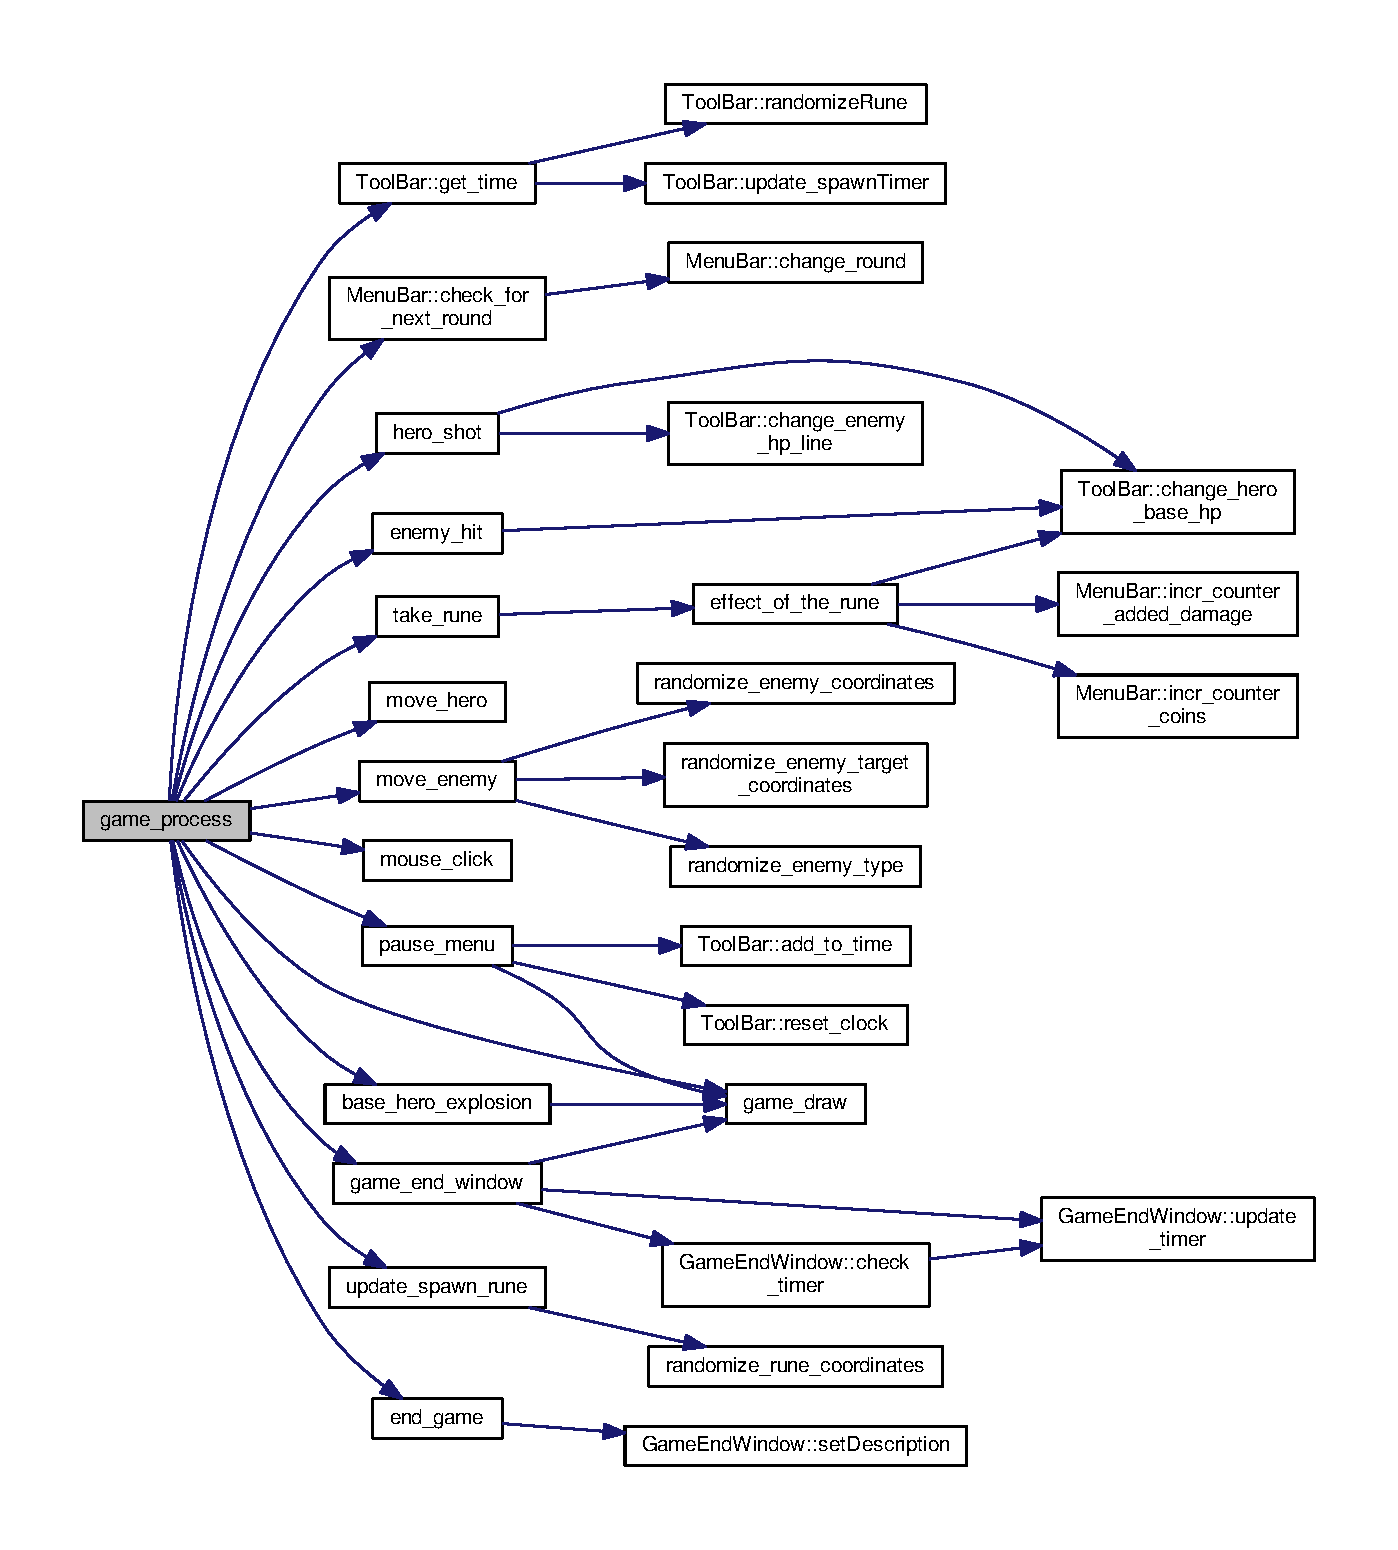
\includegraphics[width=350pt]{group__mainLoop_ga9c3324e8c5f0e0ddcd96bbe89e0f7f16_cgraph}
\end{center}
\end{figure}




Граф вызова функции\+:\nopagebreak
\begin{figure}[H]
\begin{center}
\leavevmode
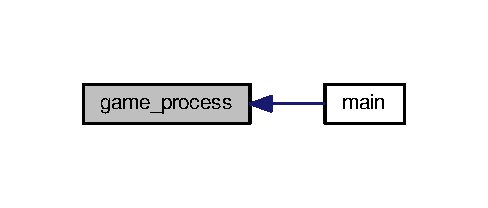
\includegraphics[width=234pt]{group__mainLoop_ga9c3324e8c5f0e0ddcd96bbe89e0f7f16_icgraph}
\end{center}
\end{figure}



\hypertarget{group__menu}{}\section{Отрисовка окон меню игры}
\label{group__menu}\index{Отрисовка окон меню игры@{Отрисовка окон меню игры}}
\subsection*{Функции}
\begin{DoxyCompactItemize}
\item 
bool \hyperlink{group__menu_ga41b04beddc9426c2999858fabc479ac0}{pause\+\_\+menu} (sf\+::\+Render\+Window \&window, \hyperlink{classMenuBar}{Menu\+Bar} \&upper\+Parametr, \hyperlink{classToolBar}{Tool\+Bar} \&lower\+Parametr, \hyperlink{classCursors}{Cursors} \&cursor, \hyperlink{classGameObject}{Game\+Object} \&object, sf\+::\+Clock \&global\+Time, sf\+::\+Clock \&game\+Time)
\begin{DoxyCompactList}\small\item\em Остановка игры и вывод меню-\/паузы \end{DoxyCompactList}\item 
bool \hyperlink{group__menu_ga11dd1886453909da6eff52362bac59b8}{mouse\+\_\+click} (\hyperlink{classMenuBar}{Menu\+Bar} \&menubar, \hyperlink{classCursors}{Cursors} \&cursor, sf\+::\+Render\+Window \&window)
\begin{DoxyCompactList}\small\item\em Обработка нажатий кнопок мыши \end{DoxyCompactList}\item 
bool \hyperlink{group__menu_ga3259e0d309cf137b40488db0226f91f6}{end\+\_\+game} (\hyperlink{classGameObject}{Game\+Object} \&object, \hyperlink{classGameEndWindow}{Game\+End\+Window} \&end\+Window)
\begin{DoxyCompactList}\small\item\em Обработка завершения игрового цроцесса \end{DoxyCompactList}\item 
void \hyperlink{group__menu_gaac2382a6b5fa5b0687116caf16837b35}{game\+\_\+end\+\_\+window} (sf\+::\+Render\+Window \&window, \hyperlink{classGameEndWindow}{Game\+End\+Window} \&end\+Window, \hyperlink{classMenuBar}{Menu\+Bar} \&upper\+Parametr, \hyperlink{classToolBar}{Tool\+Bar} \&lower\+Parametr, \hyperlink{classCursors}{Cursors} \&cursor, \hyperlink{classGameObject}{Game\+Object} \&object, sf\+::\+Clock \&global\+Time)
\begin{DoxyCompactList}\small\item\em Вывод диалогового окна \char`\"{}конец игры\char`\"{}. \end{DoxyCompactList}\item 
int \hyperlink{group__menu_gae66f6b31b5ad750f1fe042a706a4e3d4}{main} ()
\begin{DoxyCompactList}\small\item\em Отрисовка главного меню \end{DoxyCompactList}\end{DoxyCompactItemize}


\subsection{Подробное описание}


\subsection{Функции}
\index{Отрисовка окон меню игры@{Отрисовка окон меню игры}!end\+\_\+game@{end\+\_\+game}}
\index{end\+\_\+game@{end\+\_\+game}!Отрисовка окон меню игры@{Отрисовка окон меню игры}}
\subsubsection[{\texorpdfstring{end\+\_\+game(\+Game\+Object \&object, Game\+End\+Window \&end\+Window)}{end_game(GameObject &object, GameEndWindow &endWindow)}}]{\setlength{\rightskip}{0pt plus 5cm}bool end\+\_\+game (
\begin{DoxyParamCaption}
\item[{{\bf Game\+Object} \&}]{object, }
\item[{{\bf Game\+End\+Window} \&}]{end\+Window}
\end{DoxyParamCaption}
)}\hypertarget{group__menu_ga3259e0d309cf137b40488db0226f91f6}{}\label{group__menu_ga3259e0d309cf137b40488db0226f91f6}


Обработка завершения игрового цроцесса 


\begin{DoxyParams}{Аргументы}
{\em object} & класса Game\+Objects с игровыми объектами \\
\hline
{\em end\+Window} & \\
\hline
\end{DoxyParams}
\begin{DoxyReturn}{Возвращает}
флаг о заверщении игры\+: true-\/игра завершина, false-\/игра продолжается 
\end{DoxyReturn}


Граф вызовов\+:\nopagebreak
\begin{figure}[H]
\begin{center}
\leavevmode
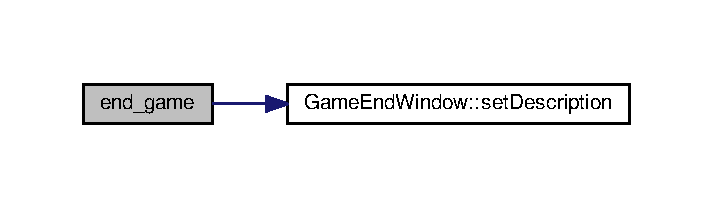
\includegraphics[width=342pt]{group__menu_ga3259e0d309cf137b40488db0226f91f6_cgraph}
\end{center}
\end{figure}




Граф вызова функции\+:\nopagebreak
\begin{figure}[H]
\begin{center}
\leavevmode
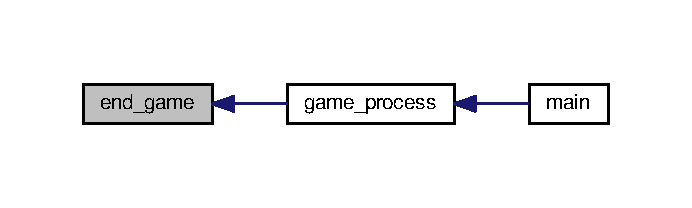
\includegraphics[width=332pt]{group__menu_ga3259e0d309cf137b40488db0226f91f6_icgraph}
\end{center}
\end{figure}


\index{Отрисовка окон меню игры@{Отрисовка окон меню игры}!game\+\_\+end\+\_\+window@{game\+\_\+end\+\_\+window}}
\index{game\+\_\+end\+\_\+window@{game\+\_\+end\+\_\+window}!Отрисовка окон меню игры@{Отрисовка окон меню игры}}
\subsubsection[{\texorpdfstring{game\+\_\+end\+\_\+window(sf\+::\+Render\+Window \&window, Game\+End\+Window \&end\+Window, Menu\+Bar \&upper\+Parametr, Tool\+Bar \&lower\+Parametr, Cursors \&cursor, Game\+Object \&object, sf\+::\+Clock \&global\+Time)}{game_end_window(sf::RenderWindow &window, GameEndWindow &endWindow, MenuBar &upperParametr, ToolBar &lowerParametr, Cursors &cursor, GameObject &object, sf::Clock &globalTime)}}]{\setlength{\rightskip}{0pt plus 5cm}void game\+\_\+end\+\_\+window (
\begin{DoxyParamCaption}
\item[{sf\+::\+Render\+Window \&}]{window, }
\item[{{\bf Game\+End\+Window} \&}]{end\+Window, }
\item[{{\bf Menu\+Bar} \&}]{upper\+Parametr, }
\item[{{\bf Tool\+Bar} \&}]{lower\+Parametr, }
\item[{{\bf Cursors} \&}]{cursor, }
\item[{{\bf Game\+Object} \&}]{object, }
\item[{sf\+::\+Clock \&}]{global\+Time}
\end{DoxyParamCaption}
)}\hypertarget{group__menu_gaac2382a6b5fa5b0687116caf16837b35}{}\label{group__menu_gaac2382a6b5fa5b0687116caf16837b35}


Вывод диалогового окна \char`\"{}конец игры\char`\"{}. 


\begin{DoxyParams}{Аргументы}
{\em window} & окно игры \\
\hline
{\em end\+Window} & объект класса \hyperlink{classGameEndWindow}{Game\+End\+Window} c параметрами диалогового окна, выводимого при завершении игры \\
\hline
{\em upper\+Parametr} & объект класса \hyperlink{classMenuBar}{Menu\+Bar} с параметрами верхней полоски полоски(меню бара) на экране игрового процесса \\
\hline
{\em lower\+Parametr} & объект класса Toolbar с параметрами нижней полоски(тулбара) на экране игрового процесса \\
\hline
{\em cursor} & объект класса \hyperlink{classCursors}{Cursors} для отображения кастомного курсора в ркне игры \\
\hline
{\em object} & класса Game\+Objects с игровыми объектамим \\
\hline
{\em global\+Time} & таймер игры \\
\hline
{\em game\+Time} & таймер для привязки к передвижениям игровых объектов с целью снижения нагрузки на прцессор \\
\hline
\end{DoxyParams}
\begin{DoxyReturn}{Возвращает}
none 
\end{DoxyReturn}


Граф вызовов\+:\nopagebreak
\begin{figure}[H]
\begin{center}
\leavevmode
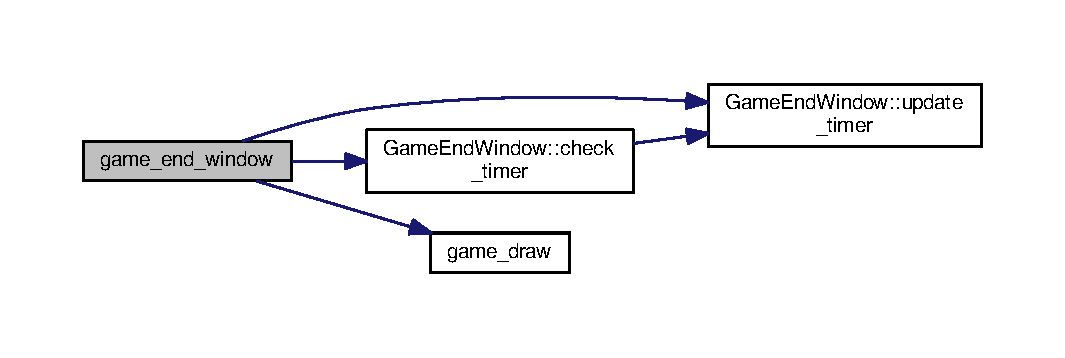
\includegraphics[width=350pt]{group__menu_gaac2382a6b5fa5b0687116caf16837b35_cgraph}
\end{center}
\end{figure}




Граф вызова функции\+:\nopagebreak
\begin{figure}[H]
\begin{center}
\leavevmode
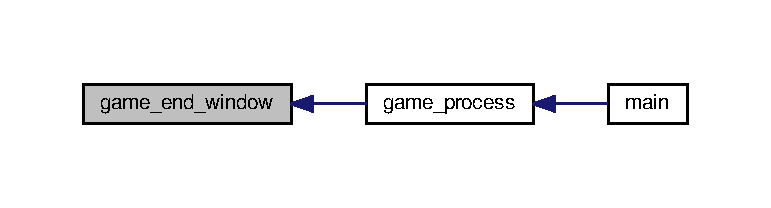
\includegraphics[width=350pt]{group__menu_gaac2382a6b5fa5b0687116caf16837b35_icgraph}
\end{center}
\end{figure}


\index{Отрисовка окон меню игры@{Отрисовка окон меню игры}!main@{main}}
\index{main@{main}!Отрисовка окон меню игры@{Отрисовка окон меню игры}}
\subsubsection[{\texorpdfstring{main()}{main()}}]{\setlength{\rightskip}{0pt plus 5cm}int main (
\begin{DoxyParamCaption}
{}
\end{DoxyParamCaption}
)}\hypertarget{group__menu_gae66f6b31b5ad750f1fe042a706a4e3d4}{}\label{group__menu_gae66f6b31b5ad750f1fe042a706a4e3d4}


Отрисовка главного меню 



Граф вызовов\+:\nopagebreak
\begin{figure}[H]
\begin{center}
\leavevmode
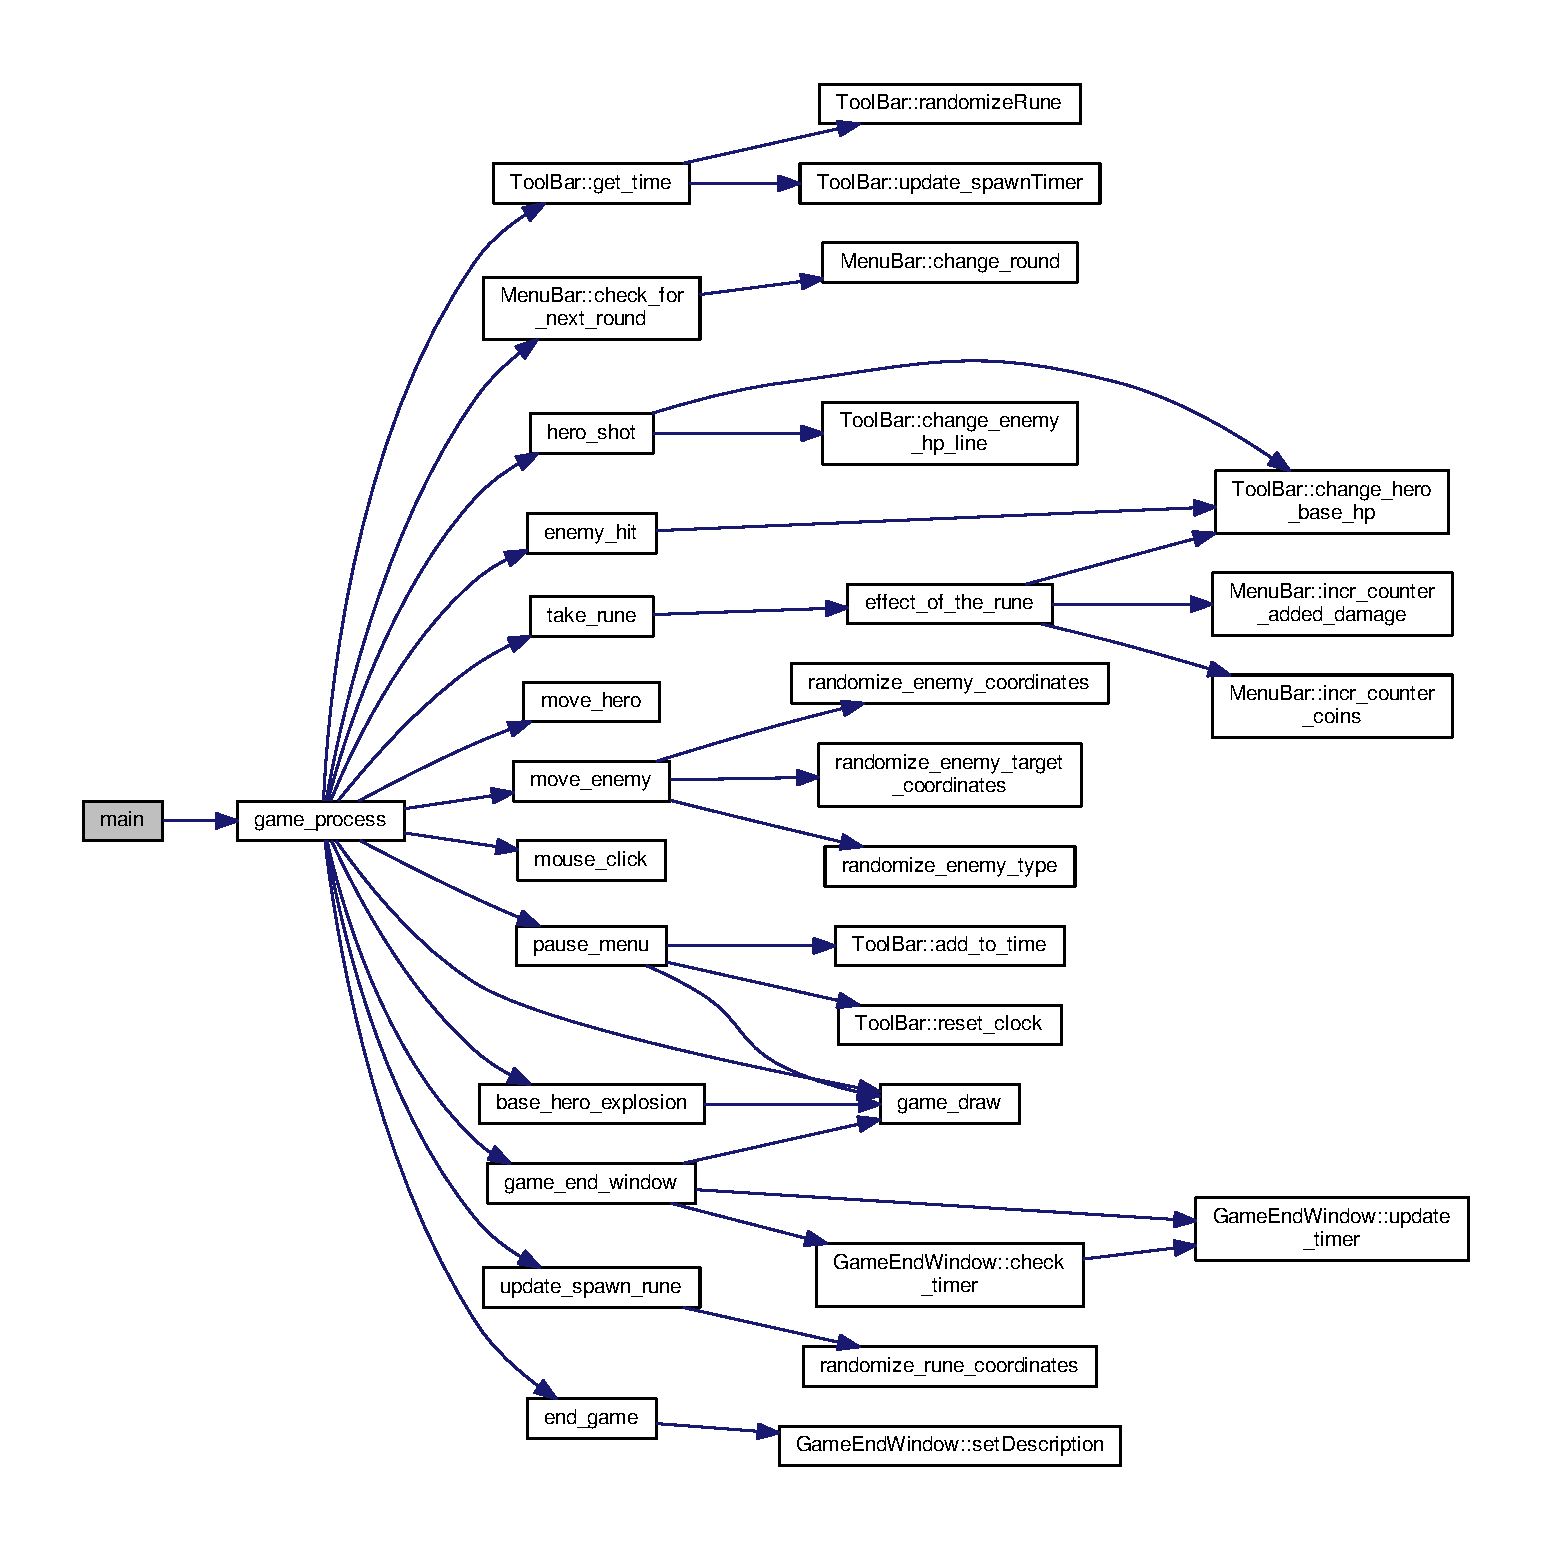
\includegraphics[width=350pt]{group__menu_gae66f6b31b5ad750f1fe042a706a4e3d4_cgraph}
\end{center}
\end{figure}


\index{Отрисовка окон меню игры@{Отрисовка окон меню игры}!mouse\+\_\+click@{mouse\+\_\+click}}
\index{mouse\+\_\+click@{mouse\+\_\+click}!Отрисовка окон меню игры@{Отрисовка окон меню игры}}
\subsubsection[{\texorpdfstring{mouse\+\_\+click(\+Menu\+Bar \&menubar, Cursors \&cursor, sf\+::\+Render\+Window \&window)}{mouse_click(MenuBar &menubar, Cursors &cursor, sf::RenderWindow &window)}}]{\setlength{\rightskip}{0pt plus 5cm}bool mouse\+\_\+click (
\begin{DoxyParamCaption}
\item[{{\bf Menu\+Bar} \&}]{menubar, }
\item[{{\bf Cursors} \&}]{cursor, }
\item[{sf\+::\+Render\+Window \&}]{window}
\end{DoxyParamCaption}
)}\hypertarget{group__menu_ga11dd1886453909da6eff52362bac59b8}{}\label{group__menu_ga11dd1886453909da6eff52362bac59b8}


Обработка нажатий кнопок мыши 


\begin{DoxyParams}{Аргументы}
{\em menubar} & объект класса \hyperlink{classMenuBar}{Menu\+Bar} с параметрами верхней полоски полоски(меню бара) на экране игрового процесса \\
\hline
{\em cursor} & объект класса \hyperlink{classCursors}{Cursors} для отображения кастомного курсора в ркне игры \\
\hline
{\em window} & окно игры \\
\hline
\end{DoxyParams}
\begin{DoxyReturn}{Возвращает}
флаг о нажатии кнопки паузы\+: true-\/кнопка нажата, false-\/кнопка не нажата 
\end{DoxyReturn}


Граф вызова функции\+:\nopagebreak
\begin{figure}[H]
\begin{center}
\leavevmode
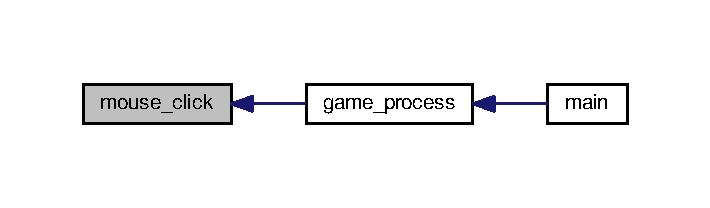
\includegraphics[width=341pt]{group__menu_ga11dd1886453909da6eff52362bac59b8_icgraph}
\end{center}
\end{figure}


\index{Отрисовка окон меню игры@{Отрисовка окон меню игры}!pause\+\_\+menu@{pause\+\_\+menu}}
\index{pause\+\_\+menu@{pause\+\_\+menu}!Отрисовка окон меню игры@{Отрисовка окон меню игры}}
\subsubsection[{\texorpdfstring{pause\+\_\+menu(sf\+::\+Render\+Window \&window, Menu\+Bar \&upper\+Parametr, Tool\+Bar \&lower\+Parametr, Cursors \&cursor, Game\+Object \&object, sf\+::\+Clock \&global\+Time, sf\+::\+Clock \&game\+Time)}{pause_menu(sf::RenderWindow &window, MenuBar &upperParametr, ToolBar &lowerParametr, Cursors &cursor, GameObject &object, sf::Clock &globalTime, sf::Clock &gameTime)}}]{\setlength{\rightskip}{0pt plus 5cm}bool pause\+\_\+menu (
\begin{DoxyParamCaption}
\item[{sf\+::\+Render\+Window \&}]{window, }
\item[{{\bf Menu\+Bar} \&}]{upper\+Parametr, }
\item[{{\bf Tool\+Bar} \&}]{lower\+Parametr, }
\item[{{\bf Cursors} \&}]{cursor, }
\item[{{\bf Game\+Object} \&}]{object, }
\item[{sf\+::\+Clock \&}]{global\+Time, }
\item[{sf\+::\+Clock \&}]{game\+Time}
\end{DoxyParamCaption}
)}\hypertarget{group__menu_ga41b04beddc9426c2999858fabc479ac0}{}\label{group__menu_ga41b04beddc9426c2999858fabc479ac0}


Остановка игры и вывод меню-\/паузы 


\begin{DoxyParams}{Аргументы}
{\em window} & окно игры \\
\hline
{\em upper\+Parametr} & объект класса \hyperlink{classMenuBar}{Menu\+Bar} с параметрами верхней полоски полоски(меню бара) на экране игрового процесса \\
\hline
{\em lower\+Parametr} & объект класса Toolbar с параметрами нижней полоски(тулбара) на экране игрового процесса \\
\hline
{\em cursor} & объект класса \hyperlink{classCursors}{Cursors} для отображения кастомного курсора в ркне игры \\
\hline
{\em object} & класса Game\+Objects с игровыми объектами \\
\hline
{\em global\+Time} & таймер игры \\
\hline
{\em game\+Time} & таймер для привязки к передвижениям игровых объектов с целью снижения нагрузки на прцессор \\
\hline
\end{DoxyParams}
\begin{DoxyReturn}{Возвращает}
флаг о нажатой кнопке в меню \char`\"{}Пауза\char`\"{}\+: true-\/была нажата кнопка \char`\"{}выход в главное меню\char`\"{}, false-\/была нажата кнопка \char`\"{}продолжить игру\char`\"{} 
\end{DoxyReturn}


Граф вызовов\+:\nopagebreak
\begin{figure}[H]
\begin{center}
\leavevmode
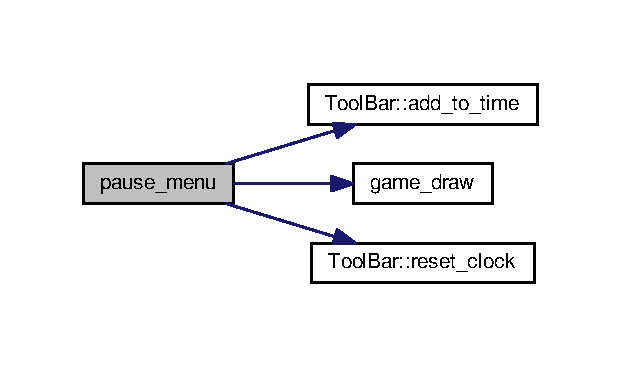
\includegraphics[width=298pt]{group__menu_ga41b04beddc9426c2999858fabc479ac0_cgraph}
\end{center}
\end{figure}




Граф вызова функции\+:\nopagebreak
\begin{figure}[H]
\begin{center}
\leavevmode
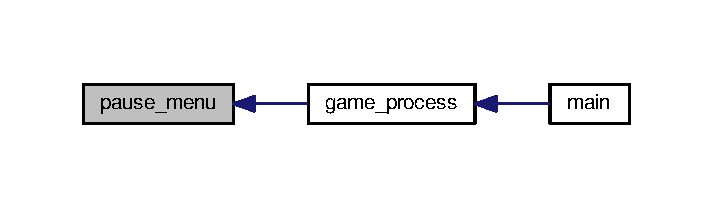
\includegraphics[width=342pt]{group__menu_ga41b04beddc9426c2999858fabc479ac0_icgraph}
\end{center}
\end{figure}



\hypertarget{group__heroBaseHandler}{}\section{Обработчики главного героя и базы}
\label{group__heroBaseHandler}\index{Обработчики главного героя и базы@{Обработчики главного героя и базы}}
\subsection*{Функции}
\begin{DoxyCompactItemize}
\item 
void \hyperlink{group__heroBaseHandler_ga3eed5602a3e229026dfc84af49007688}{move\+\_\+hero} (\hyperlink{classGameObject}{Game\+Object} \&object, float time, int flag)
\begin{DoxyCompactList}\small\item\em Передвижение главного героя в окне игрового процесса \end{DoxyCompactList}\item 
void \hyperlink{group__heroBaseHandler_gab2905c57e79ad2fcc3e51dd7fd5916dc}{hero\+\_\+shot} (\hyperlink{classGameObject}{Game\+Object} \&object, \hyperlink{classMenuBar}{Menu\+Bar} \&menubar, \hyperlink{classToolBar}{Tool\+Bar} \&toolbar, float time, sf\+::\+Render\+Window \&window)
\begin{DoxyCompactList}\small\item\em Обработка выстрелов главного героя и последующее отслеживание взаимодействий пули с объектами \end{DoxyCompactList}\item 
void \hyperlink{group__heroBaseHandler_ga4b8f8d1c761e24c0a8480a7489d349d1}{base\+\_\+hero\+\_\+explosion} (sf\+::\+Render\+Window \&window, \hyperlink{classMenuBar}{Menu\+Bar} \&upper\+Parametr, \hyperlink{classToolBar}{Tool\+Bar} \&lower\+Parametr, \hyperlink{classCursors}{Cursors} \&cursor, \hyperlink{classGameObject}{Game\+Object} \&object, sf\+::\+Clock \&game\+Time)
\begin{DoxyCompactList}\small\item\em Отрисовка и анимация взрыва базы \end{DoxyCompactList}\end{DoxyCompactItemize}


\subsection{Подробное описание}


\subsection{Функции}
\index{Обработчики главного героя и базы@{Обработчики главного героя и базы}!base\+\_\+hero\+\_\+explosion@{base\+\_\+hero\+\_\+explosion}}
\index{base\+\_\+hero\+\_\+explosion@{base\+\_\+hero\+\_\+explosion}!Обработчики главного героя и базы@{Обработчики главного героя и базы}}
\subsubsection[{\texorpdfstring{base\+\_\+hero\+\_\+explosion(sf\+::\+Render\+Window \&window, Menu\+Bar \&upper\+Parametr, Tool\+Bar \&lower\+Parametr, Cursors \&cursor, Game\+Object \&object, sf\+::\+Clock \&game\+Time)}{base_hero_explosion(sf::RenderWindow &window, MenuBar &upperParametr, ToolBar &lowerParametr, Cursors &cursor, GameObject &object, sf::Clock &gameTime)}}]{\setlength{\rightskip}{0pt plus 5cm}void base\+\_\+hero\+\_\+explosion (
\begin{DoxyParamCaption}
\item[{sf\+::\+Render\+Window \&}]{window, }
\item[{{\bf Menu\+Bar} \&}]{upper\+Parametr, }
\item[{{\bf Tool\+Bar} \&}]{lower\+Parametr, }
\item[{{\bf Cursors} \&}]{cursor, }
\item[{{\bf Game\+Object} \&}]{object, }
\item[{sf\+::\+Clock \&}]{game\+Time}
\end{DoxyParamCaption}
)}\hypertarget{group__heroBaseHandler_ga4b8f8d1c761e24c0a8480a7489d349d1}{}\label{group__heroBaseHandler_ga4b8f8d1c761e24c0a8480a7489d349d1}


Отрисовка и анимация взрыва базы 


\begin{DoxyParams}{Аргументы}
{\em window} & окно игры \\
\hline
{\em upper\+Parametr} & объект класса \hyperlink{classMenuBar}{Menu\+Bar} с параметрами верхней полоски полоски(меню бара) на экране игрового процесса \\
\hline
{\em lower\+Parametr} & объект класса Toolbar с параметрами нижней полоски(тулбара) на экране игрового процесса \\
\hline
{\em cursor} & объект класса \hyperlink{classCursors}{Cursors} для отображения кастомного курсора в ркне игры \\
\hline
{\em object} & класса Game\+Objects с игровыми объектами \\
\hline
{\em gamel\+Time} & таймер для привязки к передвижениям игровых объектов с целью снижения нагрузки на прцессор \\
\hline
\end{DoxyParams}
\begin{DoxyReturn}{Возвращает}
none 
\end{DoxyReturn}


Граф вызовов\+:\nopagebreak
\begin{figure}[H]
\begin{center}
\leavevmode
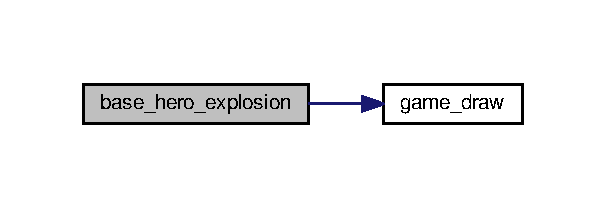
\includegraphics[width=291pt]{group__heroBaseHandler_ga4b8f8d1c761e24c0a8480a7489d349d1_cgraph}
\end{center}
\end{figure}




Граф вызова функции\+:\nopagebreak
\begin{figure}[H]
\begin{center}
\leavevmode
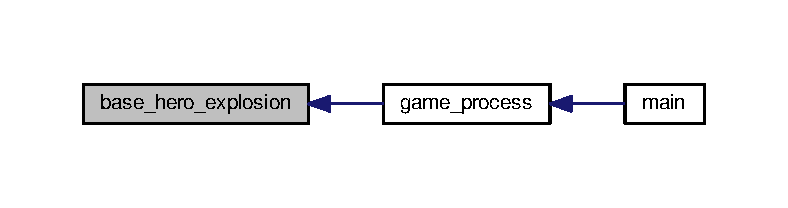
\includegraphics[width=350pt]{group__heroBaseHandler_ga4b8f8d1c761e24c0a8480a7489d349d1_icgraph}
\end{center}
\end{figure}


\index{Обработчики главного героя и базы@{Обработчики главного героя и базы}!hero\+\_\+shot@{hero\+\_\+shot}}
\index{hero\+\_\+shot@{hero\+\_\+shot}!Обработчики главного героя и базы@{Обработчики главного героя и базы}}
\subsubsection[{\texorpdfstring{hero\+\_\+shot(\+Game\+Object \&object, Menu\+Bar \&menubar, Tool\+Bar \&toolbar, float time, sf\+::\+Render\+Window \&window)}{hero_shot(GameObject &object, MenuBar &menubar, ToolBar &toolbar, float time, sf::RenderWindow &window)}}]{\setlength{\rightskip}{0pt plus 5cm}void hero\+\_\+shot (
\begin{DoxyParamCaption}
\item[{{\bf Game\+Object} \&}]{object, }
\item[{{\bf Menu\+Bar} \&}]{menubar, }
\item[{{\bf Tool\+Bar} \&}]{toolbar, }
\item[{float}]{time, }
\item[{sf\+::\+Render\+Window \&}]{window}
\end{DoxyParamCaption}
)}\hypertarget{group__heroBaseHandler_gab2905c57e79ad2fcc3e51dd7fd5916dc}{}\label{group__heroBaseHandler_gab2905c57e79ad2fcc3e51dd7fd5916dc}


Обработка выстрелов главного героя и последующее отслеживание взаимодействий пули с объектами 


\begin{DoxyParams}{Аргументы}
{\em object} & класса Game\+Objects с игровыми объектами \\
\hline
{\em menubar} & объект класса \hyperlink{classMenuBar}{Menu\+Bar} с параметрами верхней полоски полоски(меню бара) на экране игрового процесса \\
\hline
{\em toolbar} & объект класса Toolbar с параметрами нижней полоски(тулбара) на экране игрового процесса \\
\hline
{\em time} & врямя работы предыдущего цикла игры \\
\hline
{\em window} & окно игры \\
\hline
\end{DoxyParams}
\begin{DoxyReturn}{Возвращает}
none 
\end{DoxyReturn}


Граф вызовов\+:\nopagebreak
\begin{figure}[H]
\begin{center}
\leavevmode
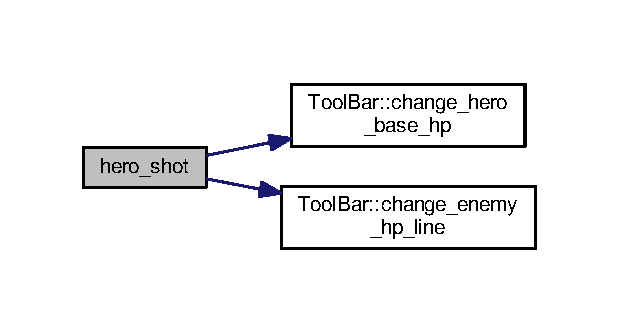
\includegraphics[width=297pt]{group__heroBaseHandler_gab2905c57e79ad2fcc3e51dd7fd5916dc_cgraph}
\end{center}
\end{figure}




Граф вызова функции\+:\nopagebreak
\begin{figure}[H]
\begin{center}
\leavevmode
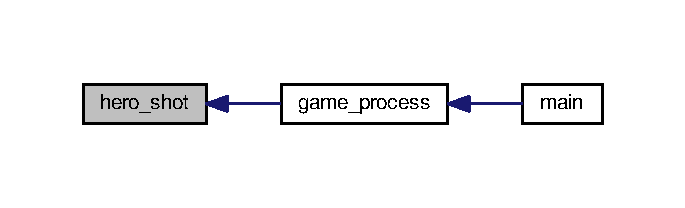
\includegraphics[width=329pt]{group__heroBaseHandler_gab2905c57e79ad2fcc3e51dd7fd5916dc_icgraph}
\end{center}
\end{figure}


\index{Обработчики главного героя и базы@{Обработчики главного героя и базы}!move\+\_\+hero@{move\+\_\+hero}}
\index{move\+\_\+hero@{move\+\_\+hero}!Обработчики главного героя и базы@{Обработчики главного героя и базы}}
\subsubsection[{\texorpdfstring{move\+\_\+hero(\+Game\+Object \&object, float time, int flag)}{move_hero(GameObject &object, float time, int flag)}}]{\setlength{\rightskip}{0pt plus 5cm}void move\+\_\+hero (
\begin{DoxyParamCaption}
\item[{{\bf Game\+Object} \&}]{object, }
\item[{float}]{time, }
\item[{int}]{flag}
\end{DoxyParamCaption}
)}\hypertarget{group__heroBaseHandler_ga3eed5602a3e229026dfc84af49007688}{}\label{group__heroBaseHandler_ga3eed5602a3e229026dfc84af49007688}


Передвижение главного героя в окне игрового процесса 


\begin{DoxyParams}{Аргументы}
{\em object} & класса Game\+Objects с игровыми объектами \\
\hline
{\em time} & врямя работы предыдущего цикла игры \\
\hline
{\em flag} & флаг для тестирования функции \\
\hline
\end{DoxyParams}
\begin{DoxyReturn}{Возвращает}
none 
\end{DoxyReturn}


Граф вызова функции\+:\nopagebreak
\begin{figure}[H]
\begin{center}
\leavevmode
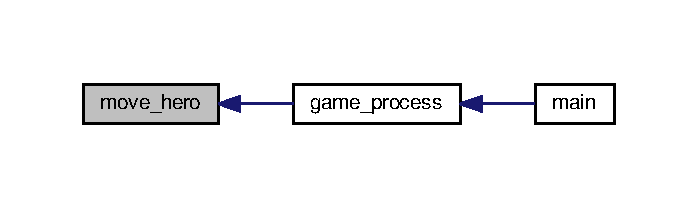
\includegraphics[width=335pt]{group__heroBaseHandler_ga3eed5602a3e229026dfc84af49007688_icgraph}
\end{center}
\end{figure}



\hypertarget{group__enemyHandler}{}\section{Обработчики противников}
\label{group__enemyHandler}\index{Обработчики противников@{Обработчики противников}}
\subsection*{Функции}
\begin{DoxyCompactItemize}
\item 
void \hyperlink{group__enemyHandler_ga95a06e0efaa583439b679f0b28419ba9}{move\+\_\+enemy} (\hyperlink{classGameObject}{Game\+Object} \&object, float time, std\+::minstd\+\_\+rand \&simple\+\_\+rand)
\begin{DoxyCompactList}\small\item\em Обработка движений противников по карте игрового процесса \end{DoxyCompactList}\item 
void \hyperlink{group__enemyHandler_ga6965d0b7bc93883e1089dd9a326a584a}{enemy\+\_\+hit} (\hyperlink{classGameObject}{Game\+Object} \&object, \hyperlink{classToolBar}{Tool\+Bar} \&toolbar, float time)
\begin{DoxyCompactList}\small\item\em Обработка атаки врагов на карте игрового процесса \end{DoxyCompactList}\item 
sf\+::\+Vector3f \hyperlink{group__enemyHandler_gacc579aee4d796c717e760e72c1c75ec3}{randomize\+\_\+enemy\+\_\+coordinates} (\hyperlink{classGameObject}{Game\+Object} \&object, std\+::minstd\+\_\+rand \&simple\+\_\+rand)
\begin{DoxyCompactList}\small\item\em Случайным образом получаем координаты точки,на которой будет заспавнен противник \end{DoxyCompactList}\item 
sf\+::\+Vector2f \hyperlink{group__enemyHandler_ga778c7ea2e26eb1d80652bf61d1661fb1}{randomize\+\_\+enemy\+\_\+target\+\_\+coordinates} (\hyperlink{classGameObject}{Game\+Object} \&object, float type\+Position, std\+::minstd\+\_\+rand \&simple\+\_\+rand)
\begin{DoxyCompactList}\small\item\em Случайным образом получаем кооординаты точки,до которой противник должен дойти \end{DoxyCompactList}\item 
int \hyperlink{group__enemyHandler_ga21c57a411b6aa06a0f36c9eefab38b5b}{randomize\+\_\+enemy\+\_\+type} (std\+::minstd\+\_\+rand \&simple\+\_\+rand)
\begin{DoxyCompactList}\small\item\em Случайным образом получаем тип противника,который будет заспавнен на карте игрового процесса \end{DoxyCompactList}\end{DoxyCompactItemize}


\subsection{Подробное описание}


\subsection{Функции}
\index{Обработчики противников@{Обработчики противников}!enemy\+\_\+hit@{enemy\+\_\+hit}}
\index{enemy\+\_\+hit@{enemy\+\_\+hit}!Обработчики противников@{Обработчики противников}}
\subsubsection[{\texorpdfstring{enemy\+\_\+hit(\+Game\+Object \&object, Tool\+Bar \&toolbar, float time)}{enemy_hit(GameObject &object, ToolBar &toolbar, float time)}}]{\setlength{\rightskip}{0pt plus 5cm}void enemy\+\_\+hit (
\begin{DoxyParamCaption}
\item[{{\bf Game\+Object} \&}]{object, }
\item[{{\bf Tool\+Bar} \&}]{toolbar, }
\item[{float}]{time}
\end{DoxyParamCaption}
)}\hypertarget{group__enemyHandler_ga6965d0b7bc93883e1089dd9a326a584a}{}\label{group__enemyHandler_ga6965d0b7bc93883e1089dd9a326a584a}


Обработка атаки врагов на карте игрового процесса 


\begin{DoxyParams}{Аргументы}
{\em object} & класса Game\+Objects с игровыми объектами \\
\hline
{\em toolbar} & объект класса Toolbar с параметрами нижней полоски(тулбара) на экране игрового процесса \\
\hline
{\em time} & врямя работы предыдущего цикла игры \\
\hline
\end{DoxyParams}


Граф вызовов\+:\nopagebreak
\begin{figure}[H]
\begin{center}
\leavevmode
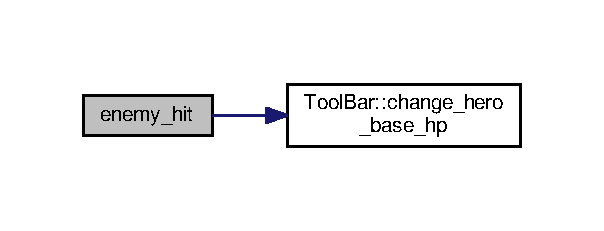
\includegraphics[width=290pt]{group__enemyHandler_ga6965d0b7bc93883e1089dd9a326a584a_cgraph}
\end{center}
\end{figure}




Граф вызова функции\+:\nopagebreak
\begin{figure}[H]
\begin{center}
\leavevmode
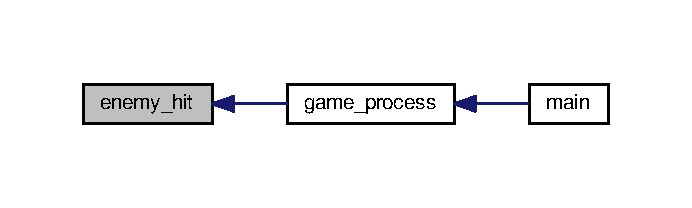
\includegraphics[width=332pt]{group__enemyHandler_ga6965d0b7bc93883e1089dd9a326a584a_icgraph}
\end{center}
\end{figure}


\index{Обработчики противников@{Обработчики противников}!move\+\_\+enemy@{move\+\_\+enemy}}
\index{move\+\_\+enemy@{move\+\_\+enemy}!Обработчики противников@{Обработчики противников}}
\subsubsection[{\texorpdfstring{move\+\_\+enemy(\+Game\+Object \&object, float time, std\+::minstd\+\_\+rand \&simple\+\_\+rand)}{move_enemy(GameObject &object, float time, std::minstd_rand &simple_rand)}}]{\setlength{\rightskip}{0pt plus 5cm}void move\+\_\+enemy (
\begin{DoxyParamCaption}
\item[{{\bf Game\+Object} \&}]{object, }
\item[{float}]{time, }
\item[{std\+::minstd\+\_\+rand \&}]{simple\+\_\+rand}
\end{DoxyParamCaption}
)}\hypertarget{group__enemyHandler_ga95a06e0efaa583439b679f0b28419ba9}{}\label{group__enemyHandler_ga95a06e0efaa583439b679f0b28419ba9}


Обработка движений противников по карте игрового процесса 

\begin{DoxyRefDesc}{Необходимо сделать}
\item[\hyperlink{todo__todo000002}{Необходимо сделать}]Требуется улучшить обработчик взаимодействия с объектами на карте\end{DoxyRefDesc}



\begin{DoxyParams}{Аргументы}
{\em object} & класса Game\+Objects с игровыми объектами \\
\hline
{\em time} & врямя работы предыдущего цикла игры \\
\hline
\end{DoxyParams}
\begin{DoxyReturn}{Возвращает}
none 
\end{DoxyReturn}


Граф вызовов\+:\nopagebreak
\begin{figure}[H]
\begin{center}
\leavevmode
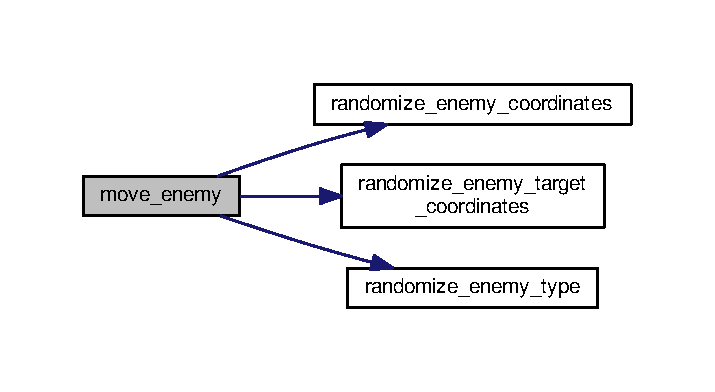
\includegraphics[width=343pt]{group__enemyHandler_ga95a06e0efaa583439b679f0b28419ba9_cgraph}
\end{center}
\end{figure}




Граф вызова функции\+:\nopagebreak
\begin{figure}[H]
\begin{center}
\leavevmode
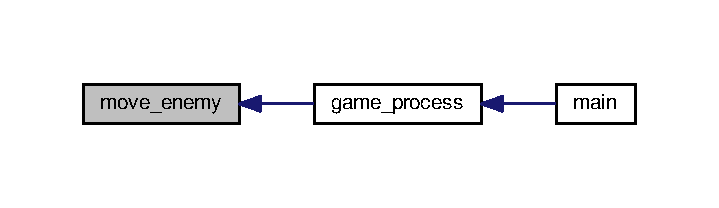
\includegraphics[width=345pt]{group__enemyHandler_ga95a06e0efaa583439b679f0b28419ba9_icgraph}
\end{center}
\end{figure}


\index{Обработчики противников@{Обработчики противников}!randomize\+\_\+enemy\+\_\+coordinates@{randomize\+\_\+enemy\+\_\+coordinates}}
\index{randomize\+\_\+enemy\+\_\+coordinates@{randomize\+\_\+enemy\+\_\+coordinates}!Обработчики противников@{Обработчики противников}}
\subsubsection[{\texorpdfstring{randomize\+\_\+enemy\+\_\+coordinates(\+Game\+Object \&object, std\+::minstd\+\_\+rand \&simple\+\_\+rand)}{randomize_enemy_coordinates(GameObject &object, std::minstd_rand &simple_rand)}}]{\setlength{\rightskip}{0pt plus 5cm}sf\+::\+Vector3f randomize\+\_\+enemy\+\_\+coordinates (
\begin{DoxyParamCaption}
\item[{{\bf Game\+Object} \&}]{object, }
\item[{std\+::minstd\+\_\+rand \&}]{simple\+\_\+rand}
\end{DoxyParamCaption}
)}\hypertarget{group__enemyHandler_gacc579aee4d796c717e760e72c1c75ec3}{}\label{group__enemyHandler_gacc579aee4d796c717e760e72c1c75ec3}


Случайным образом получаем координаты точки,на которой будет заспавнен противник 


\begin{DoxyParams}{Аргументы}
{\em object} & класса Game\+Objects с игровыми объектамим \\
\hline
{\em simple\+\_\+rand} & рандомайзер для получения случайных велечин \\
\hline
\end{DoxyParams}
\begin{DoxyReturn}{Возвращает}

\end{DoxyReturn}


Граф вызова функции\+:\nopagebreak
\begin{figure}[H]
\begin{center}
\leavevmode
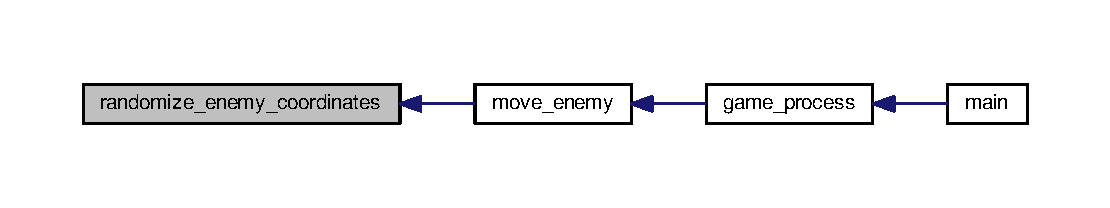
\includegraphics[width=350pt]{group__enemyHandler_gacc579aee4d796c717e760e72c1c75ec3_icgraph}
\end{center}
\end{figure}


\index{Обработчики противников@{Обработчики противников}!randomize\+\_\+enemy\+\_\+target\+\_\+coordinates@{randomize\+\_\+enemy\+\_\+target\+\_\+coordinates}}
\index{randomize\+\_\+enemy\+\_\+target\+\_\+coordinates@{randomize\+\_\+enemy\+\_\+target\+\_\+coordinates}!Обработчики противников@{Обработчики противников}}
\subsubsection[{\texorpdfstring{randomize\+\_\+enemy\+\_\+target\+\_\+coordinates(\+Game\+Object \&object, float type\+Position, std\+::minstd\+\_\+rand \&simple\+\_\+rand)}{randomize_enemy_target_coordinates(GameObject &object, float typePosition, std::minstd_rand &simple_rand)}}]{\setlength{\rightskip}{0pt plus 5cm}sf\+::\+Vector2f randomize\+\_\+enemy\+\_\+target\+\_\+coordinates (
\begin{DoxyParamCaption}
\item[{{\bf Game\+Object} \&}]{object, }
\item[{float}]{type\+Position, }
\item[{std\+::minstd\+\_\+rand \&}]{simple\+\_\+rand}
\end{DoxyParamCaption}
)}\hypertarget{group__enemyHandler_ga778c7ea2e26eb1d80652bf61d1661fb1}{}\label{group__enemyHandler_ga778c7ea2e26eb1d80652bf61d1661fb1}


Случайным образом получаем кооординаты точки,до которой противник должен дойти 


\begin{DoxyParams}{Аргументы}
{\em object} & класса Game\+Objects с игровыми объектамим \\
\hline
{\em type\+Position} & область спавна противника\+: 0-\/сверху от базы, 1-\/справа от базы, 2-\/снизу от базы, 3-\/слева от базы\\
\hline
{\em simple\+\_\+rand} & рандомайзер для получения случайных велечин \\
\hline
\end{DoxyParams}
\begin{DoxyReturn}{Возвращает}

\end{DoxyReturn}


Граф вызова функции\+:\nopagebreak
\begin{figure}[H]
\begin{center}
\leavevmode
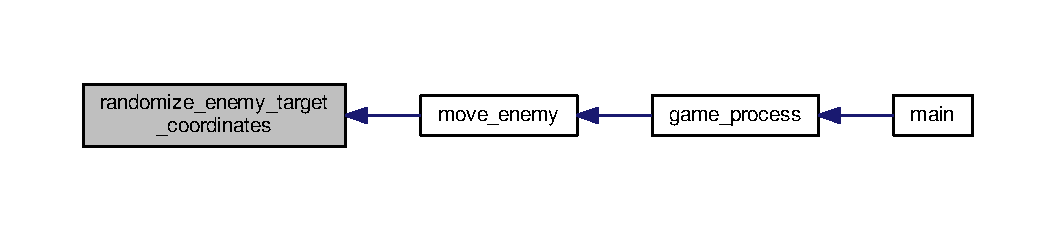
\includegraphics[width=350pt]{group__enemyHandler_ga778c7ea2e26eb1d80652bf61d1661fb1_icgraph}
\end{center}
\end{figure}


\index{Обработчики противников@{Обработчики противников}!randomize\+\_\+enemy\+\_\+type@{randomize\+\_\+enemy\+\_\+type}}
\index{randomize\+\_\+enemy\+\_\+type@{randomize\+\_\+enemy\+\_\+type}!Обработчики противников@{Обработчики противников}}
\subsubsection[{\texorpdfstring{randomize\+\_\+enemy\+\_\+type(std\+::minstd\+\_\+rand \&simple\+\_\+rand)}{randomize_enemy_type(std::minstd_rand &simple_rand)}}]{\setlength{\rightskip}{0pt plus 5cm}int randomize\+\_\+enemy\+\_\+type (
\begin{DoxyParamCaption}
\item[{std\+::minstd\+\_\+rand \&}]{simple\+\_\+rand}
\end{DoxyParamCaption}
)}\hypertarget{group__enemyHandler_ga21c57a411b6aa06a0f36c9eefab38b5b}{}\label{group__enemyHandler_ga21c57a411b6aa06a0f36c9eefab38b5b}


Случайным образом получаем тип противника,который будет заспавнен на карте игрового процесса 


\begin{DoxyParams}{Аргументы}
{\em object} & класса Game\+Objects с игровыми объектамим \\
\hline
{\em simple\+\_\+rand} & рандомайзер для получения случайных велечин \\
\hline
\end{DoxyParams}
\begin{DoxyReturn}{Возвращает}

\end{DoxyReturn}


Граф вызова функции\+:\nopagebreak
\begin{figure}[H]
\begin{center}
\leavevmode
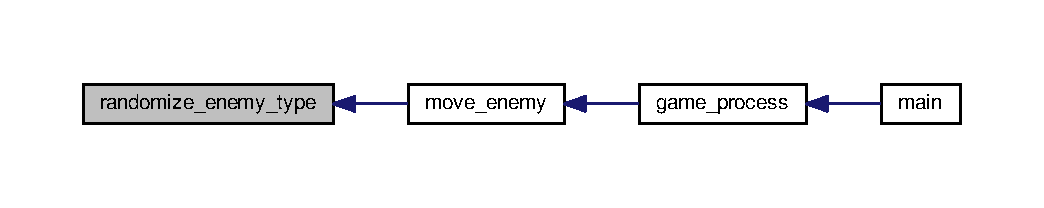
\includegraphics[width=350pt]{group__enemyHandler_ga21c57a411b6aa06a0f36c9eefab38b5b_icgraph}
\end{center}
\end{figure}



\hypertarget{group__runeHandler}{}\section{Обработчики рун}
\label{group__runeHandler}\index{Обработчики рун@{Обработчики рун}}
\subsection*{Функции}
\begin{DoxyCompactItemize}
\item 
void \hyperlink{group__runeHandler_ga813bbb2330c07f4bf303406c4efab35d}{update\+\_\+spawn\+\_\+rune} (\hyperlink{classGameObject}{Game\+Object} \&object, \hyperlink{classToolBar}{Tool\+Bar} \&toolbar, float \&rune\+U\+P\+D\+A\+T\+Etime, float \&time, std\+::minstd\+\_\+rand \&simple\+\_\+rand)
\begin{DoxyCompactList}\small\item\em Анимация руны и её вывод на карту игрового процесса \end{DoxyCompactList}\item 
void \hyperlink{group__runeHandler_gaf2bb7b78f028e61a0c6674cd9b976a8c}{take\+\_\+rune} (\hyperlink{classGameObject}{Game\+Object} \&object, \hyperlink{classToolBar}{Tool\+Bar} \&toolbar, \hyperlink{classMenuBar}{Menu\+Bar} \&menubar)
\begin{DoxyCompactList}\small\item\em Обработка взаимодействия главного героя с заспавненной руной на карте игрового процесса \end{DoxyCompactList}\item 
void \hyperlink{group__runeHandler_ga0078b36ac662e224e1913996193c1c98}{effect\+\_\+of\+\_\+the\+\_\+rune} (\hyperlink{classGameObject}{Game\+Object} \&object, \hyperlink{classToolBar}{Tool\+Bar} \&toolbar, \hyperlink{classMenuBar}{Menu\+Bar} \&menubar)
\begin{DoxyCompactList}\small\item\em Обрабатывается эффект применения руны в соответствии с её типом \end{DoxyCompactList}\item 
void \hyperlink{group__runeHandler_gad3bb6254181bfa4913a3ec9a0f206f69}{randomize\+\_\+rune\+\_\+coordinates} (\hyperlink{classGameObject}{Game\+Object} \&object, \hyperlink{classToolBar}{Tool\+Bar} \&toolbar, std\+::minstd\+\_\+rand \&simple\+\_\+rand)
\begin{DoxyCompactList}\small\item\em Выбираются случайным образом координаты руны для отображения на карте \end{DoxyCompactList}\end{DoxyCompactItemize}


\subsection{Подробное описание}


\subsection{Функции}
\index{Обработчики рун@{Обработчики рун}!effect\+\_\+of\+\_\+the\+\_\+rune@{effect\+\_\+of\+\_\+the\+\_\+rune}}
\index{effect\+\_\+of\+\_\+the\+\_\+rune@{effect\+\_\+of\+\_\+the\+\_\+rune}!Обработчики рун@{Обработчики рун}}
\subsubsection[{\texorpdfstring{effect\+\_\+of\+\_\+the\+\_\+rune(\+Game\+Object \&object, Tool\+Bar \&toolbar, Menu\+Bar \&menubar)}{effect_of_the_rune(GameObject &object, ToolBar &toolbar, MenuBar &menubar)}}]{\setlength{\rightskip}{0pt plus 5cm}void effect\+\_\+of\+\_\+the\+\_\+rune (
\begin{DoxyParamCaption}
\item[{{\bf Game\+Object} \&}]{object, }
\item[{{\bf Tool\+Bar} \&}]{toolbar, }
\item[{{\bf Menu\+Bar} \&}]{menubar}
\end{DoxyParamCaption}
)}\hypertarget{group__runeHandler_ga0078b36ac662e224e1913996193c1c98}{}\label{group__runeHandler_ga0078b36ac662e224e1913996193c1c98}


Обрабатывается эффект применения руны в соответствии с её типом 


\begin{DoxyParams}{Аргументы}
{\em объект} & класса Game\+Objects с игровыми объектами \\
\hline
{\em toolbar} & объект класса Toolbar с параметрами нижней полоски(тулбара) на экране игрового процесса \\
\hline
{\em menubar} & объект класса \hyperlink{classMenuBar}{Menu\+Bar} с параметрами верхней полоски полоски(меню бара) на экране игрового процесса \\
\hline
\end{DoxyParams}
\begin{DoxyReturn}{Возвращает}
none 
\end{DoxyReturn}


Граф вызовов\+:\nopagebreak
\begin{figure}[H]
\begin{center}
\leavevmode
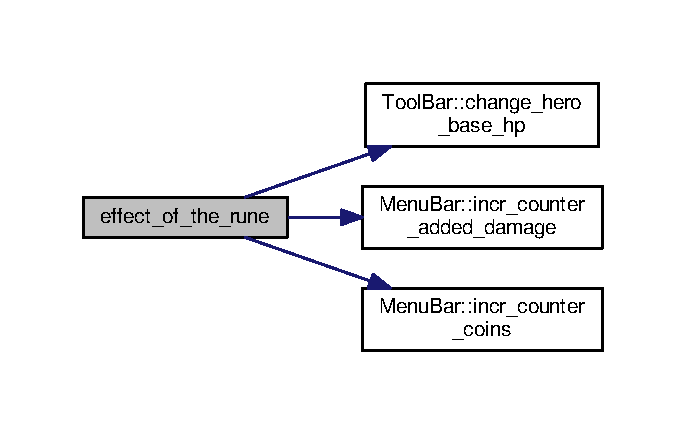
\includegraphics[width=329pt]{group__runeHandler_ga0078b36ac662e224e1913996193c1c98_cgraph}
\end{center}
\end{figure}




Граф вызова функции\+:\nopagebreak
\begin{figure}[H]
\begin{center}
\leavevmode
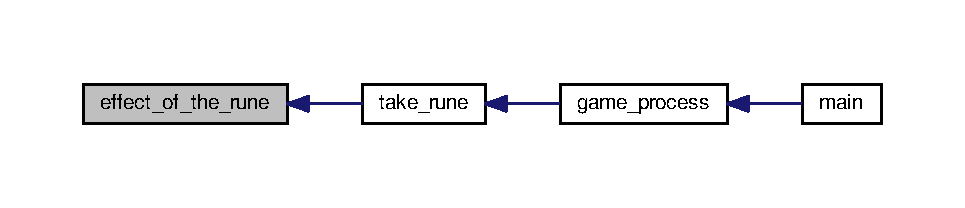
\includegraphics[width=350pt]{group__runeHandler_ga0078b36ac662e224e1913996193c1c98_icgraph}
\end{center}
\end{figure}


\index{Обработчики рун@{Обработчики рун}!randomize\+\_\+rune\+\_\+coordinates@{randomize\+\_\+rune\+\_\+coordinates}}
\index{randomize\+\_\+rune\+\_\+coordinates@{randomize\+\_\+rune\+\_\+coordinates}!Обработчики рун@{Обработчики рун}}
\subsubsection[{\texorpdfstring{randomize\+\_\+rune\+\_\+coordinates(\+Game\+Object \&object, Tool\+Bar \&toolbar, std\+::minstd\+\_\+rand \&simple\+\_\+rand)}{randomize_rune_coordinates(GameObject &object, ToolBar &toolbar, std::minstd_rand &simple_rand)}}]{\setlength{\rightskip}{0pt plus 5cm}void randomize\+\_\+rune\+\_\+coordinates (
\begin{DoxyParamCaption}
\item[{{\bf Game\+Object} \&}]{object, }
\item[{{\bf Tool\+Bar} \&}]{toolbar, }
\item[{std\+::minstd\+\_\+rand \&}]{simple\+\_\+rand}
\end{DoxyParamCaption}
)}\hypertarget{group__runeHandler_gad3bb6254181bfa4913a3ec9a0f206f69}{}\label{group__runeHandler_gad3bb6254181bfa4913a3ec9a0f206f69}


Выбираются случайным образом координаты руны для отображения на карте 


\begin{DoxyParams}{Аргументы}
{\em object} & объект класса Game\+Objects с игровыми объектами \\
\hline
{\em toolbar} & объект класса \hyperlink{classToolBar}{Tool\+Bar} с параметрами нижней полоски(тулбара) на экране игрового процесса \\
\hline
{\em simple\+\_\+rand} & рандомайзер для получения случайных велечин \\
\hline
\end{DoxyParams}
\begin{DoxyReturn}{Возвращает}
none 
\end{DoxyReturn}


Граф вызова функции\+:\nopagebreak
\begin{figure}[H]
\begin{center}
\leavevmode
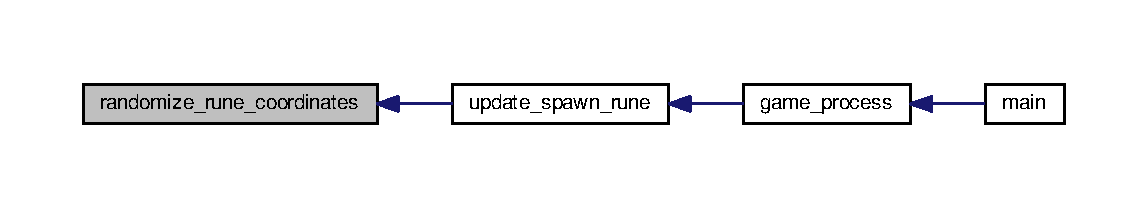
\includegraphics[width=350pt]{group__runeHandler_gad3bb6254181bfa4913a3ec9a0f206f69_icgraph}
\end{center}
\end{figure}


\index{Обработчики рун@{Обработчики рун}!take\+\_\+rune@{take\+\_\+rune}}
\index{take\+\_\+rune@{take\+\_\+rune}!Обработчики рун@{Обработчики рун}}
\subsubsection[{\texorpdfstring{take\+\_\+rune(\+Game\+Object \&object, Tool\+Bar \&toolbar, Menu\+Bar \&menubar)}{take_rune(GameObject &object, ToolBar &toolbar, MenuBar &menubar)}}]{\setlength{\rightskip}{0pt plus 5cm}void take\+\_\+rune (
\begin{DoxyParamCaption}
\item[{{\bf Game\+Object} \&}]{object, }
\item[{{\bf Tool\+Bar} \&}]{toolbar, }
\item[{{\bf Menu\+Bar} \&}]{menubar}
\end{DoxyParamCaption}
)}\hypertarget{group__runeHandler_gaf2bb7b78f028e61a0c6674cd9b976a8c}{}\label{group__runeHandler_gaf2bb7b78f028e61a0c6674cd9b976a8c}


Обработка взаимодействия главного героя с заспавненной руной на карте игрового процесса 


\begin{DoxyParams}{Аргументы}
{\em object} & класса Game\+Objects с игровыми объектами \\
\hline
{\em toolbar} & объект класса Toolbar с параметрами нижней полоски(тулбара) на экране игрового процесса \\
\hline
{\em menubar} & объект класса \hyperlink{classMenuBar}{Menu\+Bar} с параметрами верхней полоски полоски(меню бара) на экране игрового процесса \\
\hline
\end{DoxyParams}
\begin{DoxyReturn}{Возвращает}
none 
\end{DoxyReturn}


Граф вызовов\+:\nopagebreak
\begin{figure}[H]
\begin{center}
\leavevmode
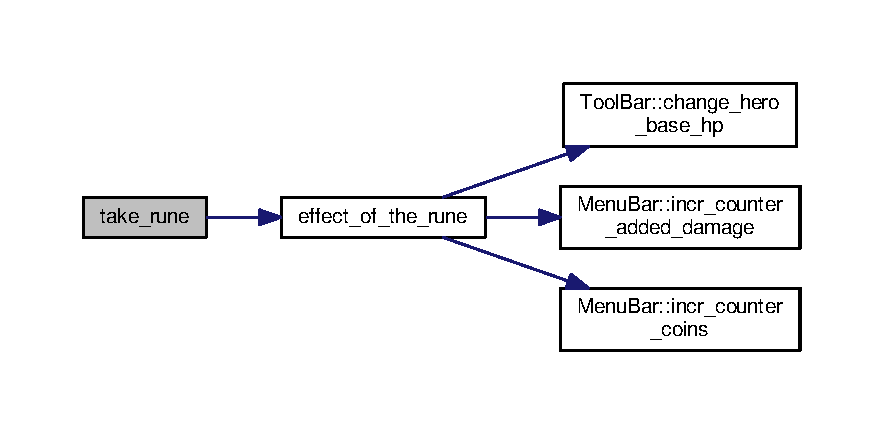
\includegraphics[width=350pt]{group__runeHandler_gaf2bb7b78f028e61a0c6674cd9b976a8c_cgraph}
\end{center}
\end{figure}




Граф вызова функции\+:\nopagebreak
\begin{figure}[H]
\begin{center}
\leavevmode
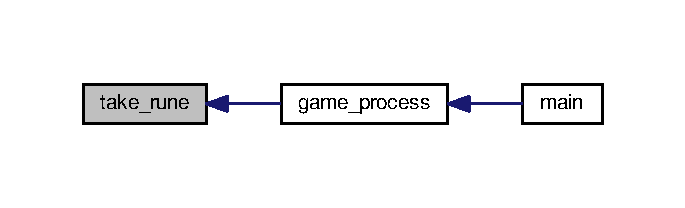
\includegraphics[width=329pt]{group__runeHandler_gaf2bb7b78f028e61a0c6674cd9b976a8c_icgraph}
\end{center}
\end{figure}


\index{Обработчики рун@{Обработчики рун}!update\+\_\+spawn\+\_\+rune@{update\+\_\+spawn\+\_\+rune}}
\index{update\+\_\+spawn\+\_\+rune@{update\+\_\+spawn\+\_\+rune}!Обработчики рун@{Обработчики рун}}
\subsubsection[{\texorpdfstring{update\+\_\+spawn\+\_\+rune(\+Game\+Object \&object, Tool\+Bar \&toolbar, float \&rune\+U\+P\+D\+A\+T\+Etime, float \&time, std\+::minstd\+\_\+rand \&simple\+\_\+rand)}{update_spawn_rune(GameObject &object, ToolBar &toolbar, float &runeUPDATEtime, float &time, std::minstd_rand &simple_rand)}}]{\setlength{\rightskip}{0pt plus 5cm}void update\+\_\+spawn\+\_\+rune (
\begin{DoxyParamCaption}
\item[{{\bf Game\+Object} \&}]{object, }
\item[{{\bf Tool\+Bar} \&}]{toolbar, }
\item[{float \&}]{rune\+U\+P\+D\+A\+T\+Etime, }
\item[{float \&}]{time, }
\item[{std\+::minstd\+\_\+rand \&}]{simple\+\_\+rand}
\end{DoxyParamCaption}
)}\hypertarget{group__runeHandler_ga813bbb2330c07f4bf303406c4efab35d}{}\label{group__runeHandler_ga813bbb2330c07f4bf303406c4efab35d}


Анимация руны и её вывод на карту игрового процесса 


\begin{DoxyParams}{Аргументы}
{\em object} & класса Game\+Objects с игровыми объектами \\
\hline
{\em toolbar} & объект класса Toolbar с параметрами нижней полоски(тулбара) на экране игрового процесса \\
\hline
{\em rune\+U\+P\+D\+A\+T\+Etime} & время с прошлого спавна руны \\
\hline
{\em time} & врямя работы предыдущего цикла игры \\
\hline
{\em simple\+\_\+rand} & рандомайзер для получения случайных велечин \\
\hline
\end{DoxyParams}
\begin{DoxyReturn}{Возвращает}
none 
\end{DoxyReturn}


Граф вызовов\+:\nopagebreak
\begin{figure}[H]
\begin{center}
\leavevmode
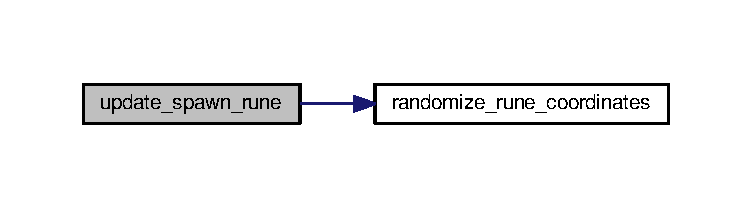
\includegraphics[width=350pt]{group__runeHandler_ga813bbb2330c07f4bf303406c4efab35d_cgraph}
\end{center}
\end{figure}




Граф вызова функции\+:\nopagebreak
\begin{figure}[H]
\begin{center}
\leavevmode
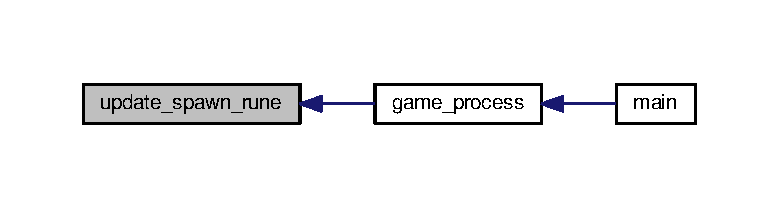
\includegraphics[width=350pt]{group__runeHandler_ga813bbb2330c07f4bf303406c4efab35d_icgraph}
\end{center}
\end{figure}



\chapter{Структуры данных}
\hypertarget{classGameObject_1_1Base}{}\section{Класс Game\+Object\+:\+:Base}
\label{classGameObject_1_1Base}\index{Game\+Object\+::\+Base@{Game\+Object\+::\+Base}}


The \hyperlink{classGameObject_1_1Base}{Base} class.  




{\ttfamily \#include $<$game\+\_\+objects.\+h$>$}

\subsection*{Открытые члены}
\begin{DoxyCompactItemize}
\item 
\hyperlink{classGameObject_1_1Base_a31c0f6c9e600dacf73e76673b1a13c1e}{Base} ()
\end{DoxyCompactItemize}
\subsection*{Поля данных}
\begin{DoxyCompactItemize}
\item 
sf\+::\+Sprite \hyperlink{classGameObject_1_1Base_ab8f40bafa7b9290ffa287df2b75eb49f}{sprite}
\item 
sf\+::\+Sprite \hyperlink{classGameObject_1_1Base_a585759d198272b88275e6757d0cb9b2e}{base\+\_\+roof}
\item 
int \hyperlink{classGameObject_1_1Base_aafab029af0a095c1b7751b94a630d5a8}{health}
\item 
bool \hyperlink{classGameObject_1_1Base_ad5b542f2b0694adbcdf26a088ab7394a}{live}
\item 
float \hyperlink{classGameObject_1_1Base_a253d1b270383dde6a83bcced281df00e}{box\+\_\+x}
\item 
float \hyperlink{classGameObject_1_1Base_a6524bcc9f2c8581932f7bd474ddecc63}{box\+\_\+y}
\item 
float \hyperlink{classGameObject_1_1Base_ab8c68f4cc3270595be6867e2d0c4c8a4}{w}
\item 
float \hyperlink{classGameObject_1_1Base_afbfe39f23eea3c89426e1053ec1a064e}{h}
\end{DoxyCompactItemize}


\subsection{Подробное описание}
The \hyperlink{classGameObject_1_1Base}{Base} class. 

\subsection{Конструктор(ы)}
\index{Game\+Object\+::\+Base@{Game\+Object\+::\+Base}!Base@{Base}}
\index{Base@{Base}!Game\+Object\+::\+Base@{Game\+Object\+::\+Base}}
\subsubsection[{\texorpdfstring{Base()}{Base()}}]{\setlength{\rightskip}{0pt plus 5cm}Game\+Object\+::\+Base\+::\+Base (
\begin{DoxyParamCaption}
{}
\end{DoxyParamCaption}
)\hspace{0.3cm}{\ttfamily [inline]}}\hypertarget{classGameObject_1_1Base_a31c0f6c9e600dacf73e76673b1a13c1e}{}\label{classGameObject_1_1Base_a31c0f6c9e600dacf73e76673b1a13c1e}


\subsection{Поля}
\index{Game\+Object\+::\+Base@{Game\+Object\+::\+Base}!base\+\_\+roof@{base\+\_\+roof}}
\index{base\+\_\+roof@{base\+\_\+roof}!Game\+Object\+::\+Base@{Game\+Object\+::\+Base}}
\subsubsection[{\texorpdfstring{base\+\_\+roof}{base_roof}}]{\setlength{\rightskip}{0pt plus 5cm}sf\+::\+Sprite Game\+Object\+::\+Base\+::base\+\_\+roof}\hypertarget{classGameObject_1_1Base_a585759d198272b88275e6757d0cb9b2e}{}\label{classGameObject_1_1Base_a585759d198272b88275e6757d0cb9b2e}
\index{Game\+Object\+::\+Base@{Game\+Object\+::\+Base}!box\+\_\+x@{box\+\_\+x}}
\index{box\+\_\+x@{box\+\_\+x}!Game\+Object\+::\+Base@{Game\+Object\+::\+Base}}
\subsubsection[{\texorpdfstring{box\+\_\+x}{box_x}}]{\setlength{\rightskip}{0pt plus 5cm}float Game\+Object\+::\+Base\+::box\+\_\+x}\hypertarget{classGameObject_1_1Base_a253d1b270383dde6a83bcced281df00e}{}\label{classGameObject_1_1Base_a253d1b270383dde6a83bcced281df00e}
\index{Game\+Object\+::\+Base@{Game\+Object\+::\+Base}!box\+\_\+y@{box\+\_\+y}}
\index{box\+\_\+y@{box\+\_\+y}!Game\+Object\+::\+Base@{Game\+Object\+::\+Base}}
\subsubsection[{\texorpdfstring{box\+\_\+y}{box_y}}]{\setlength{\rightskip}{0pt plus 5cm}float Game\+Object\+::\+Base\+::box\+\_\+y}\hypertarget{classGameObject_1_1Base_a6524bcc9f2c8581932f7bd474ddecc63}{}\label{classGameObject_1_1Base_a6524bcc9f2c8581932f7bd474ddecc63}
\index{Game\+Object\+::\+Base@{Game\+Object\+::\+Base}!h@{h}}
\index{h@{h}!Game\+Object\+::\+Base@{Game\+Object\+::\+Base}}
\subsubsection[{\texorpdfstring{h}{h}}]{\setlength{\rightskip}{0pt plus 5cm}float Game\+Object\+::\+Base\+::h}\hypertarget{classGameObject_1_1Base_afbfe39f23eea3c89426e1053ec1a064e}{}\label{classGameObject_1_1Base_afbfe39f23eea3c89426e1053ec1a064e}
\index{Game\+Object\+::\+Base@{Game\+Object\+::\+Base}!health@{health}}
\index{health@{health}!Game\+Object\+::\+Base@{Game\+Object\+::\+Base}}
\subsubsection[{\texorpdfstring{health}{health}}]{\setlength{\rightskip}{0pt plus 5cm}int Game\+Object\+::\+Base\+::health}\hypertarget{classGameObject_1_1Base_aafab029af0a095c1b7751b94a630d5a8}{}\label{classGameObject_1_1Base_aafab029af0a095c1b7751b94a630d5a8}
\index{Game\+Object\+::\+Base@{Game\+Object\+::\+Base}!live@{live}}
\index{live@{live}!Game\+Object\+::\+Base@{Game\+Object\+::\+Base}}
\subsubsection[{\texorpdfstring{live}{live}}]{\setlength{\rightskip}{0pt plus 5cm}bool Game\+Object\+::\+Base\+::live}\hypertarget{classGameObject_1_1Base_ad5b542f2b0694adbcdf26a088ab7394a}{}\label{classGameObject_1_1Base_ad5b542f2b0694adbcdf26a088ab7394a}
\index{Game\+Object\+::\+Base@{Game\+Object\+::\+Base}!sprite@{sprite}}
\index{sprite@{sprite}!Game\+Object\+::\+Base@{Game\+Object\+::\+Base}}
\subsubsection[{\texorpdfstring{sprite}{sprite}}]{\setlength{\rightskip}{0pt plus 5cm}sf\+::\+Sprite Game\+Object\+::\+Base\+::sprite}\hypertarget{classGameObject_1_1Base_ab8f40bafa7b9290ffa287df2b75eb49f}{}\label{classGameObject_1_1Base_ab8f40bafa7b9290ffa287df2b75eb49f}
\index{Game\+Object\+::\+Base@{Game\+Object\+::\+Base}!w@{w}}
\index{w@{w}!Game\+Object\+::\+Base@{Game\+Object\+::\+Base}}
\subsubsection[{\texorpdfstring{w}{w}}]{\setlength{\rightskip}{0pt plus 5cm}float Game\+Object\+::\+Base\+::w}\hypertarget{classGameObject_1_1Base_ab8c68f4cc3270595be6867e2d0c4c8a4}{}\label{classGameObject_1_1Base_ab8c68f4cc3270595be6867e2d0c4c8a4}

\hypertarget{classGameObject_1_1BaseExplosion}{}\section{Класс Game\+Object\+:\+:Base\+Explosion}
\label{classGameObject_1_1BaseExplosion}\index{Game\+Object\+::\+Base\+Explosion@{Game\+Object\+::\+Base\+Explosion}}


The \hyperlink{classGameObject_1_1BaseExplosion}{Base\+Explosion} class.  




{\ttfamily \#include $<$game\+\_\+objects.\+h$>$}

\subsection*{Открытые члены}
\begin{DoxyCompactItemize}
\item 
\hyperlink{classGameObject_1_1BaseExplosion_aa7fa02ce95e2dd9cd91fe845ec99668f}{Base\+Explosion} ()
\item 
bool \hyperlink{classGameObject_1_1BaseExplosion_ae87cb3cb807223fcbc113a785886cc7a}{update\+Frame} ()
\end{DoxyCompactItemize}
\subsection*{Поля данных}
\begin{DoxyCompactItemize}
\item 
sf\+::\+Sprite \hyperlink{classGameObject_1_1BaseExplosion_affea6677e855c484ce9627b6cc455cda}{sprite}
\item 
float \hyperlink{classGameObject_1_1BaseExplosion_ade5becc1e6e278fd529df839286daa48}{w}
\item 
float \hyperlink{classGameObject_1_1BaseExplosion_a1ee54235dfe58e3a75c19721135d0d87}{h}
\item 
float \hyperlink{classGameObject_1_1BaseExplosion_a8209c6eb059c2e9391c10048064b0781}{row}
\item 
float \hyperlink{classGameObject_1_1BaseExplosion_ab035aca99e6764293c5b83a6405c7c97}{colomn}
\end{DoxyCompactItemize}


\subsection{Подробное описание}
The \hyperlink{classGameObject_1_1BaseExplosion}{Base\+Explosion} class. 

\subsection{Конструктор(ы)}
\index{Game\+Object\+::\+Base\+Explosion@{Game\+Object\+::\+Base\+Explosion}!Base\+Explosion@{Base\+Explosion}}
\index{Base\+Explosion@{Base\+Explosion}!Game\+Object\+::\+Base\+Explosion@{Game\+Object\+::\+Base\+Explosion}}
\subsubsection[{\texorpdfstring{Base\+Explosion()}{BaseExplosion()}}]{\setlength{\rightskip}{0pt plus 5cm}Game\+Object\+::\+Base\+Explosion\+::\+Base\+Explosion (
\begin{DoxyParamCaption}
{}
\end{DoxyParamCaption}
)\hspace{0.3cm}{\ttfamily [inline]}}\hypertarget{classGameObject_1_1BaseExplosion_aa7fa02ce95e2dd9cd91fe845ec99668f}{}\label{classGameObject_1_1BaseExplosion_aa7fa02ce95e2dd9cd91fe845ec99668f}


\subsection{Методы}
\index{Game\+Object\+::\+Base\+Explosion@{Game\+Object\+::\+Base\+Explosion}!update\+Frame@{update\+Frame}}
\index{update\+Frame@{update\+Frame}!Game\+Object\+::\+Base\+Explosion@{Game\+Object\+::\+Base\+Explosion}}
\subsubsection[{\texorpdfstring{update\+Frame()}{updateFrame()}}]{\setlength{\rightskip}{0pt plus 5cm}bool Game\+Object\+::\+Base\+Explosion\+::update\+Frame (
\begin{DoxyParamCaption}
{}
\end{DoxyParamCaption}
)\hspace{0.3cm}{\ttfamily [inline]}}\hypertarget{classGameObject_1_1BaseExplosion_ae87cb3cb807223fcbc113a785886cc7a}{}\label{classGameObject_1_1BaseExplosion_ae87cb3cb807223fcbc113a785886cc7a}


\subsection{Поля}
\index{Game\+Object\+::\+Base\+Explosion@{Game\+Object\+::\+Base\+Explosion}!colomn@{colomn}}
\index{colomn@{colomn}!Game\+Object\+::\+Base\+Explosion@{Game\+Object\+::\+Base\+Explosion}}
\subsubsection[{\texorpdfstring{colomn}{colomn}}]{\setlength{\rightskip}{0pt plus 5cm}float Game\+Object\+::\+Base\+Explosion\+::colomn}\hypertarget{classGameObject_1_1BaseExplosion_ab035aca99e6764293c5b83a6405c7c97}{}\label{classGameObject_1_1BaseExplosion_ab035aca99e6764293c5b83a6405c7c97}
\index{Game\+Object\+::\+Base\+Explosion@{Game\+Object\+::\+Base\+Explosion}!h@{h}}
\index{h@{h}!Game\+Object\+::\+Base\+Explosion@{Game\+Object\+::\+Base\+Explosion}}
\subsubsection[{\texorpdfstring{h}{h}}]{\setlength{\rightskip}{0pt plus 5cm}float Game\+Object\+::\+Base\+Explosion\+::h}\hypertarget{classGameObject_1_1BaseExplosion_a1ee54235dfe58e3a75c19721135d0d87}{}\label{classGameObject_1_1BaseExplosion_a1ee54235dfe58e3a75c19721135d0d87}
\index{Game\+Object\+::\+Base\+Explosion@{Game\+Object\+::\+Base\+Explosion}!row@{row}}
\index{row@{row}!Game\+Object\+::\+Base\+Explosion@{Game\+Object\+::\+Base\+Explosion}}
\subsubsection[{\texorpdfstring{row}{row}}]{\setlength{\rightskip}{0pt plus 5cm}float Game\+Object\+::\+Base\+Explosion\+::row}\hypertarget{classGameObject_1_1BaseExplosion_a8209c6eb059c2e9391c10048064b0781}{}\label{classGameObject_1_1BaseExplosion_a8209c6eb059c2e9391c10048064b0781}
\index{Game\+Object\+::\+Base\+Explosion@{Game\+Object\+::\+Base\+Explosion}!sprite@{sprite}}
\index{sprite@{sprite}!Game\+Object\+::\+Base\+Explosion@{Game\+Object\+::\+Base\+Explosion}}
\subsubsection[{\texorpdfstring{sprite}{sprite}}]{\setlength{\rightskip}{0pt plus 5cm}sf\+::\+Sprite Game\+Object\+::\+Base\+Explosion\+::sprite}\hypertarget{classGameObject_1_1BaseExplosion_affea6677e855c484ce9627b6cc455cda}{}\label{classGameObject_1_1BaseExplosion_affea6677e855c484ce9627b6cc455cda}
\index{Game\+Object\+::\+Base\+Explosion@{Game\+Object\+::\+Base\+Explosion}!w@{w}}
\index{w@{w}!Game\+Object\+::\+Base\+Explosion@{Game\+Object\+::\+Base\+Explosion}}
\subsubsection[{\texorpdfstring{w}{w}}]{\setlength{\rightskip}{0pt plus 5cm}float Game\+Object\+::\+Base\+Explosion\+::w}\hypertarget{classGameObject_1_1BaseExplosion_ade5becc1e6e278fd529df839286daa48}{}\label{classGameObject_1_1BaseExplosion_ade5becc1e6e278fd529df839286daa48}

\hypertarget{classGameObject_1_1Bullet}{}\section{Класс Game\+Object\+:\+:Bullet}
\label{classGameObject_1_1Bullet}\index{Game\+Object\+::\+Bullet@{Game\+Object\+::\+Bullet}}


The \hyperlink{classGameObject_1_1Bullet}{Bullet} class.  




{\ttfamily \#include $<$game\+\_\+objects.\+h$>$}

\subsection*{Открытые члены}
\begin{DoxyCompactItemize}
\item 
\hyperlink{classGameObject_1_1Bullet_a38fedbbbe892177fee4b34c2dd9955ec}{Bullet} ()
\item 
\hyperlink{classGameObject_1_1Bullet_a5e93be5fdfe2361c85f08b53cbc14002}{Bullet} (int dir, float x, float y)
\item 
void \hyperlink{classGameObject_1_1Bullet_a68ee8b2d12e43e847b70ace7a95cf833}{update\+\_\+explosion\+\_\+coord} (float x, float y, int gun\+\_\+dir)
\item 
void \hyperlink{classGameObject_1_1Bullet_afd9561c0d310ff22205dc5c63f9cda56}{load\+\_\+sprite} ()
\end{DoxyCompactItemize}
\subsection*{Поля данных}
\begin{DoxyCompactItemize}
\item 
sf\+::\+Sprite \hyperlink{classGameObject_1_1Bullet_a5e219ab143176814c91e1064c495551b}{sprite}
\item 
int \hyperlink{classGameObject_1_1Bullet_a859aff17279d7d762ff8fd6a89372ae4}{damage}
\item 
bool \hyperlink{classGameObject_1_1Bullet_acfafc84be2b90c0bd0a5a0161c7e55ee}{draw}
\item 
float \hyperlink{classGameObject_1_1Bullet_af4b107bb1ed2e8c5d98b3322be75e6dc}{speed}
\item 
int \hyperlink{classGameObject_1_1Bullet_ab957f45f5450884b8aaca05104305b4a}{direction}
\item 
float \hyperlink{classGameObject_1_1Bullet_a1f1402d7e00dcb529b443be5250cde13}{w}
\item 
float \hyperlink{classGameObject_1_1Bullet_adb6e34303c0f92ee177e1855bc2a3ea7}{h}
\item 
sf\+::\+Sprite \hyperlink{classGameObject_1_1Bullet_a77557b33ad1f1879683a0ff89b9bdd76}{explosion}
\item 
int \hyperlink{classGameObject_1_1Bullet_a447b3ab4306b065be824f9ecc1ddf5bf}{shot}
\end{DoxyCompactItemize}


\subsection{Подробное описание}
The \hyperlink{classGameObject_1_1Bullet}{Bullet} class. 

\subsection{Конструктор(ы)}
\index{Game\+Object\+::\+Bullet@{Game\+Object\+::\+Bullet}!Bullet@{Bullet}}
\index{Bullet@{Bullet}!Game\+Object\+::\+Bullet@{Game\+Object\+::\+Bullet}}
\subsubsection[{\texorpdfstring{Bullet()}{Bullet()}}]{\setlength{\rightskip}{0pt plus 5cm}Game\+Object\+::\+Bullet\+::\+Bullet (
\begin{DoxyParamCaption}
{}
\end{DoxyParamCaption}
)\hspace{0.3cm}{\ttfamily [inline]}}\hypertarget{classGameObject_1_1Bullet_a38fedbbbe892177fee4b34c2dd9955ec}{}\label{classGameObject_1_1Bullet_a38fedbbbe892177fee4b34c2dd9955ec}
\index{Game\+Object\+::\+Bullet@{Game\+Object\+::\+Bullet}!Bullet@{Bullet}}
\index{Bullet@{Bullet}!Game\+Object\+::\+Bullet@{Game\+Object\+::\+Bullet}}
\subsubsection[{\texorpdfstring{Bullet(int dir, float x, float y)}{Bullet(int dir, float x, float y)}}]{\setlength{\rightskip}{0pt plus 5cm}Game\+Object\+::\+Bullet\+::\+Bullet (
\begin{DoxyParamCaption}
\item[{int}]{dir, }
\item[{float}]{x, }
\item[{float}]{y}
\end{DoxyParamCaption}
)\hspace{0.3cm}{\ttfamily [inline]}}\hypertarget{classGameObject_1_1Bullet_a5e93be5fdfe2361c85f08b53cbc14002}{}\label{classGameObject_1_1Bullet_a5e93be5fdfe2361c85f08b53cbc14002}


\subsection{Методы}
\index{Game\+Object\+::\+Bullet@{Game\+Object\+::\+Bullet}!load\+\_\+sprite@{load\+\_\+sprite}}
\index{load\+\_\+sprite@{load\+\_\+sprite}!Game\+Object\+::\+Bullet@{Game\+Object\+::\+Bullet}}
\subsubsection[{\texorpdfstring{load\+\_\+sprite()}{load_sprite()}}]{\setlength{\rightskip}{0pt plus 5cm}void Game\+Object\+::\+Bullet\+::load\+\_\+sprite (
\begin{DoxyParamCaption}
{}
\end{DoxyParamCaption}
)\hspace{0.3cm}{\ttfamily [inline]}}\hypertarget{classGameObject_1_1Bullet_afd9561c0d310ff22205dc5c63f9cda56}{}\label{classGameObject_1_1Bullet_afd9561c0d310ff22205dc5c63f9cda56}
\index{Game\+Object\+::\+Bullet@{Game\+Object\+::\+Bullet}!update\+\_\+explosion\+\_\+coord@{update\+\_\+explosion\+\_\+coord}}
\index{update\+\_\+explosion\+\_\+coord@{update\+\_\+explosion\+\_\+coord}!Game\+Object\+::\+Bullet@{Game\+Object\+::\+Bullet}}
\subsubsection[{\texorpdfstring{update\+\_\+explosion\+\_\+coord(float x, float y, int gun\+\_\+dir)}{update_explosion_coord(float x, float y, int gun_dir)}}]{\setlength{\rightskip}{0pt plus 5cm}void Game\+Object\+::\+Bullet\+::update\+\_\+explosion\+\_\+coord (
\begin{DoxyParamCaption}
\item[{float}]{x, }
\item[{float}]{y, }
\item[{int}]{gun\+\_\+dir}
\end{DoxyParamCaption}
)\hspace{0.3cm}{\ttfamily [inline]}}\hypertarget{classGameObject_1_1Bullet_a68ee8b2d12e43e847b70ace7a95cf833}{}\label{classGameObject_1_1Bullet_a68ee8b2d12e43e847b70ace7a95cf833}


\subsection{Поля}
\index{Game\+Object\+::\+Bullet@{Game\+Object\+::\+Bullet}!damage@{damage}}
\index{damage@{damage}!Game\+Object\+::\+Bullet@{Game\+Object\+::\+Bullet}}
\subsubsection[{\texorpdfstring{damage}{damage}}]{\setlength{\rightskip}{0pt plus 5cm}int Game\+Object\+::\+Bullet\+::damage}\hypertarget{classGameObject_1_1Bullet_a859aff17279d7d762ff8fd6a89372ae4}{}\label{classGameObject_1_1Bullet_a859aff17279d7d762ff8fd6a89372ae4}
\index{Game\+Object\+::\+Bullet@{Game\+Object\+::\+Bullet}!direction@{direction}}
\index{direction@{direction}!Game\+Object\+::\+Bullet@{Game\+Object\+::\+Bullet}}
\subsubsection[{\texorpdfstring{direction}{direction}}]{\setlength{\rightskip}{0pt plus 5cm}int Game\+Object\+::\+Bullet\+::direction}\hypertarget{classGameObject_1_1Bullet_ab957f45f5450884b8aaca05104305b4a}{}\label{classGameObject_1_1Bullet_ab957f45f5450884b8aaca05104305b4a}
\index{Game\+Object\+::\+Bullet@{Game\+Object\+::\+Bullet}!draw@{draw}}
\index{draw@{draw}!Game\+Object\+::\+Bullet@{Game\+Object\+::\+Bullet}}
\subsubsection[{\texorpdfstring{draw}{draw}}]{\setlength{\rightskip}{0pt plus 5cm}bool Game\+Object\+::\+Bullet\+::draw}\hypertarget{classGameObject_1_1Bullet_acfafc84be2b90c0bd0a5a0161c7e55ee}{}\label{classGameObject_1_1Bullet_acfafc84be2b90c0bd0a5a0161c7e55ee}
\index{Game\+Object\+::\+Bullet@{Game\+Object\+::\+Bullet}!explosion@{explosion}}
\index{explosion@{explosion}!Game\+Object\+::\+Bullet@{Game\+Object\+::\+Bullet}}
\subsubsection[{\texorpdfstring{explosion}{explosion}}]{\setlength{\rightskip}{0pt plus 5cm}sf\+::\+Sprite Game\+Object\+::\+Bullet\+::explosion}\hypertarget{classGameObject_1_1Bullet_a77557b33ad1f1879683a0ff89b9bdd76}{}\label{classGameObject_1_1Bullet_a77557b33ad1f1879683a0ff89b9bdd76}
\index{Game\+Object\+::\+Bullet@{Game\+Object\+::\+Bullet}!h@{h}}
\index{h@{h}!Game\+Object\+::\+Bullet@{Game\+Object\+::\+Bullet}}
\subsubsection[{\texorpdfstring{h}{h}}]{\setlength{\rightskip}{0pt plus 5cm}float Game\+Object\+::\+Bullet\+::h}\hypertarget{classGameObject_1_1Bullet_adb6e34303c0f92ee177e1855bc2a3ea7}{}\label{classGameObject_1_1Bullet_adb6e34303c0f92ee177e1855bc2a3ea7}
\index{Game\+Object\+::\+Bullet@{Game\+Object\+::\+Bullet}!shot@{shot}}
\index{shot@{shot}!Game\+Object\+::\+Bullet@{Game\+Object\+::\+Bullet}}
\subsubsection[{\texorpdfstring{shot}{shot}}]{\setlength{\rightskip}{0pt plus 5cm}int Game\+Object\+::\+Bullet\+::shot}\hypertarget{classGameObject_1_1Bullet_a447b3ab4306b065be824f9ecc1ddf5bf}{}\label{classGameObject_1_1Bullet_a447b3ab4306b065be824f9ecc1ddf5bf}
\index{Game\+Object\+::\+Bullet@{Game\+Object\+::\+Bullet}!speed@{speed}}
\index{speed@{speed}!Game\+Object\+::\+Bullet@{Game\+Object\+::\+Bullet}}
\subsubsection[{\texorpdfstring{speed}{speed}}]{\setlength{\rightskip}{0pt plus 5cm}float Game\+Object\+::\+Bullet\+::speed}\hypertarget{classGameObject_1_1Bullet_af4b107bb1ed2e8c5d98b3322be75e6dc}{}\label{classGameObject_1_1Bullet_af4b107bb1ed2e8c5d98b3322be75e6dc}
\index{Game\+Object\+::\+Bullet@{Game\+Object\+::\+Bullet}!sprite@{sprite}}
\index{sprite@{sprite}!Game\+Object\+::\+Bullet@{Game\+Object\+::\+Bullet}}
\subsubsection[{\texorpdfstring{sprite}{sprite}}]{\setlength{\rightskip}{0pt plus 5cm}sf\+::\+Sprite Game\+Object\+::\+Bullet\+::sprite}\hypertarget{classGameObject_1_1Bullet_a5e219ab143176814c91e1064c495551b}{}\label{classGameObject_1_1Bullet_a5e219ab143176814c91e1064c495551b}
\index{Game\+Object\+::\+Bullet@{Game\+Object\+::\+Bullet}!w@{w}}
\index{w@{w}!Game\+Object\+::\+Bullet@{Game\+Object\+::\+Bullet}}
\subsubsection[{\texorpdfstring{w}{w}}]{\setlength{\rightskip}{0pt plus 5cm}float Game\+Object\+::\+Bullet\+::w}\hypertarget{classGameObject_1_1Bullet_a1f1402d7e00dcb529b443be5250cde13}{}\label{classGameObject_1_1Bullet_a1f1402d7e00dcb529b443be5250cde13}

\hypertarget{classGameObject_1_1Runes_1_1Coin}{}\section{Класс Game\+Object\+:\+:Runes\+:\+:Coin}
\label{classGameObject_1_1Runes_1_1Coin}\index{Game\+Object\+::\+Runes\+::\+Coin@{Game\+Object\+::\+Runes\+::\+Coin}}


The \hyperlink{classGameObject_1_1Runes_1_1Coin}{Coin} class.  




{\ttfamily \#include $<$game\+\_\+objects.\+h$>$}

\subsection*{Открытые члены}
\begin{DoxyCompactItemize}
\item 
\hyperlink{classGameObject_1_1Runes_1_1Coin_a8250430ea5ff2903c9ef3f1655a6753c}{Coin} ()
\end{DoxyCompactItemize}
\subsection*{Поля данных}
\begin{DoxyCompactItemize}
\item 
sf\+::\+Sprite \hyperlink{classGameObject_1_1Runes_1_1Coin_a43a7a13191c5cee9de71734908e0d341}{sprite}
\item 
float \hyperlink{classGameObject_1_1Runes_1_1Coin_ace3b26447f004e704b104a473856a244}{w}
\item 
float \hyperlink{classGameObject_1_1Runes_1_1Coin_aaa1f06beaa9a8aabe7fc2d0dd9536439}{h}
\item 
float \hyperlink{classGameObject_1_1Runes_1_1Coin_a6caff0a83608e0ef628bcecae8114a07}{frames}
\item 
float \hyperlink{classGameObject_1_1Runes_1_1Coin_a6a24ef9bcca0948f9073a8f8182526bb}{current\+\_\+frame}
\item 
int \hyperlink{classGameObject_1_1Runes_1_1Coin_a58cc56a3214709645c7667d3c13d9346}{value}
\end{DoxyCompactItemize}


\subsection{Подробное описание}
The \hyperlink{classGameObject_1_1Runes_1_1Coin}{Coin} class. 

\subsection{Конструктор(ы)}
\index{Game\+Object\+::\+Runes\+::\+Coin@{Game\+Object\+::\+Runes\+::\+Coin}!Coin@{Coin}}
\index{Coin@{Coin}!Game\+Object\+::\+Runes\+::\+Coin@{Game\+Object\+::\+Runes\+::\+Coin}}
\subsubsection[{\texorpdfstring{Coin()}{Coin()}}]{\setlength{\rightskip}{0pt plus 5cm}Game\+Object\+::\+Runes\+::\+Coin\+::\+Coin (
\begin{DoxyParamCaption}
{}
\end{DoxyParamCaption}
)\hspace{0.3cm}{\ttfamily [inline]}}\hypertarget{classGameObject_1_1Runes_1_1Coin_a8250430ea5ff2903c9ef3f1655a6753c}{}\label{classGameObject_1_1Runes_1_1Coin_a8250430ea5ff2903c9ef3f1655a6753c}


\subsection{Поля}
\index{Game\+Object\+::\+Runes\+::\+Coin@{Game\+Object\+::\+Runes\+::\+Coin}!current\+\_\+frame@{current\+\_\+frame}}
\index{current\+\_\+frame@{current\+\_\+frame}!Game\+Object\+::\+Runes\+::\+Coin@{Game\+Object\+::\+Runes\+::\+Coin}}
\subsubsection[{\texorpdfstring{current\+\_\+frame}{current_frame}}]{\setlength{\rightskip}{0pt plus 5cm}float Game\+Object\+::\+Runes\+::\+Coin\+::current\+\_\+frame}\hypertarget{classGameObject_1_1Runes_1_1Coin_a6a24ef9bcca0948f9073a8f8182526bb}{}\label{classGameObject_1_1Runes_1_1Coin_a6a24ef9bcca0948f9073a8f8182526bb}
\index{Game\+Object\+::\+Runes\+::\+Coin@{Game\+Object\+::\+Runes\+::\+Coin}!frames@{frames}}
\index{frames@{frames}!Game\+Object\+::\+Runes\+::\+Coin@{Game\+Object\+::\+Runes\+::\+Coin}}
\subsubsection[{\texorpdfstring{frames}{frames}}]{\setlength{\rightskip}{0pt plus 5cm}float Game\+Object\+::\+Runes\+::\+Coin\+::frames}\hypertarget{classGameObject_1_1Runes_1_1Coin_a6caff0a83608e0ef628bcecae8114a07}{}\label{classGameObject_1_1Runes_1_1Coin_a6caff0a83608e0ef628bcecae8114a07}
\index{Game\+Object\+::\+Runes\+::\+Coin@{Game\+Object\+::\+Runes\+::\+Coin}!h@{h}}
\index{h@{h}!Game\+Object\+::\+Runes\+::\+Coin@{Game\+Object\+::\+Runes\+::\+Coin}}
\subsubsection[{\texorpdfstring{h}{h}}]{\setlength{\rightskip}{0pt plus 5cm}float Game\+Object\+::\+Runes\+::\+Coin\+::h}\hypertarget{classGameObject_1_1Runes_1_1Coin_aaa1f06beaa9a8aabe7fc2d0dd9536439}{}\label{classGameObject_1_1Runes_1_1Coin_aaa1f06beaa9a8aabe7fc2d0dd9536439}
\index{Game\+Object\+::\+Runes\+::\+Coin@{Game\+Object\+::\+Runes\+::\+Coin}!sprite@{sprite}}
\index{sprite@{sprite}!Game\+Object\+::\+Runes\+::\+Coin@{Game\+Object\+::\+Runes\+::\+Coin}}
\subsubsection[{\texorpdfstring{sprite}{sprite}}]{\setlength{\rightskip}{0pt plus 5cm}sf\+::\+Sprite Game\+Object\+::\+Runes\+::\+Coin\+::sprite}\hypertarget{classGameObject_1_1Runes_1_1Coin_a43a7a13191c5cee9de71734908e0d341}{}\label{classGameObject_1_1Runes_1_1Coin_a43a7a13191c5cee9de71734908e0d341}
\index{Game\+Object\+::\+Runes\+::\+Coin@{Game\+Object\+::\+Runes\+::\+Coin}!value@{value}}
\index{value@{value}!Game\+Object\+::\+Runes\+::\+Coin@{Game\+Object\+::\+Runes\+::\+Coin}}
\subsubsection[{\texorpdfstring{value}{value}}]{\setlength{\rightskip}{0pt plus 5cm}int Game\+Object\+::\+Runes\+::\+Coin\+::value}\hypertarget{classGameObject_1_1Runes_1_1Coin_a58cc56a3214709645c7667d3c13d9346}{}\label{classGameObject_1_1Runes_1_1Coin_a58cc56a3214709645c7667d3c13d9346}
\index{Game\+Object\+::\+Runes\+::\+Coin@{Game\+Object\+::\+Runes\+::\+Coin}!w@{w}}
\index{w@{w}!Game\+Object\+::\+Runes\+::\+Coin@{Game\+Object\+::\+Runes\+::\+Coin}}
\subsubsection[{\texorpdfstring{w}{w}}]{\setlength{\rightskip}{0pt plus 5cm}float Game\+Object\+::\+Runes\+::\+Coin\+::w}\hypertarget{classGameObject_1_1Runes_1_1Coin_ace3b26447f004e704b104a473856a244}{}\label{classGameObject_1_1Runes_1_1Coin_ace3b26447f004e704b104a473856a244}

\hypertarget{classCursors}{}\section{Класс Cursors}
\label{classCursors}\index{Cursors@{Cursors}}


Хранимые параметры кастомного курсора в игре  




{\ttfamily \#include $<$cursors.\+h$>$}

\subsection*{Открытые члены}
\begin{DoxyCompactItemize}
\item 
\hyperlink{classCursors_a73625aa9a8dab4c7c2f857deaa176af3}{Cursors} ()
\end{DoxyCompactItemize}
\subsection*{Поля данных}
\begin{DoxyCompactItemize}
\item 
sf\+::\+Sprite \hyperlink{classCursors_a69303c342d2c4fbc190ae41b788bc6ac}{cursore}
\end{DoxyCompactItemize}


\subsection{Подробное описание}
Хранимые параметры кастомного курсора в игре 

\subsection{Конструктор(ы)}
\index{Cursors@{Cursors}!Cursors@{Cursors}}
\index{Cursors@{Cursors}!Cursors@{Cursors}}
\subsubsection[{\texorpdfstring{Cursors()}{Cursors()}}]{\setlength{\rightskip}{0pt plus 5cm}Cursors\+::\+Cursors (
\begin{DoxyParamCaption}
{}
\end{DoxyParamCaption}
)\hspace{0.3cm}{\ttfamily [inline]}}\hypertarget{classCursors_a73625aa9a8dab4c7c2f857deaa176af3}{}\label{classCursors_a73625aa9a8dab4c7c2f857deaa176af3}


\subsection{Поля}
\index{Cursors@{Cursors}!cursore@{cursore}}
\index{cursore@{cursore}!Cursors@{Cursors}}
\subsubsection[{\texorpdfstring{cursore}{cursore}}]{\setlength{\rightskip}{0pt plus 5cm}sf\+::\+Sprite Cursors\+::cursore}\hypertarget{classCursors_a69303c342d2c4fbc190ae41b788bc6ac}{}\label{classCursors_a69303c342d2c4fbc190ae41b788bc6ac}

\hypertarget{classGameObject_1_1Enemys}{}\section{Класс Game\+Object\+:\+:Enemys}
\label{classGameObject_1_1Enemys}\index{Game\+Object\+::\+Enemys@{Game\+Object\+::\+Enemys}}


The \hyperlink{classGameObject_1_1Enemys}{Enemys} class.  




{\ttfamily \#include $<$game\+\_\+objects.\+h$>$}

\subsection*{Структуры данных}
\begin{DoxyCompactItemize}
\item 
class \hyperlink{classGameObject_1_1Enemys_1_1EnemyTemlate}{Enemy\+Temlate}
\item 
class \hyperlink{classGameObject_1_1Enemys_1_1EnemyUpdates}{Enemy\+Updates}
\end{DoxyCompactItemize}


\subsection{Подробное описание}
The \hyperlink{classGameObject_1_1Enemys}{Enemys} class. 

\begin{DoxyRefDesc}{Необходимо сделать}
\item[\hyperlink{todo__todo000001}{Необходимо сделать}]Очень слабо реализована масштабируемость класс. Требуется упростить способ добавления новых объектов в качестве врагов. \end{DoxyRefDesc}

\hypertarget{classGameObject_1_1Enemys_1_1EnemyTemlate}{}\section{Класс Game\+Object\+:\+:Enemys\+:\+:Enemy\+Temlate}
\label{classGameObject_1_1Enemys_1_1EnemyTemlate}\index{Game\+Object\+::\+Enemys\+::\+Enemy\+Temlate@{Game\+Object\+::\+Enemys\+::\+Enemy\+Temlate}}


{\ttfamily \#include $<$game\+\_\+objects.\+h$>$}

\subsection*{Открытые члены}
\begin{DoxyCompactItemize}
\item 
void \hyperlink{classGameObject_1_1Enemys_1_1EnemyTemlate_ae65af0b44209fea4e92e5f13d2a09f6f}{load\+Sprite} (int enemy\+Index, int frme\+\_\+x, int frme\+\_\+y, int frme\+\_\+w, int frme\+\_\+h)
\item 
void \hyperlink{classGameObject_1_1Enemys_1_1EnemyTemlate_a5f9b71a23bb65baf0af246a2fd6f7439}{load\+Enemy\+Parametrs} (int enemy\+Index, int \&added\+Dmg\+In\+Perct, int \&added\+Hp\+In\+Perct)
\item 
void \hyperlink{classGameObject_1_1Enemys_1_1EnemyTemlate_afbc5887043ffe63e87a396365902cf23}{update\+M\+O\+V\+Eframe} ()
\item 
bool \hyperlink{classGameObject_1_1Enemys_1_1EnemyTemlate_ad214c3fa0f38bdb49ac63d87fa61f812}{update\+I\+D\+L\+Eframe} ()
\item 
bool \hyperlink{classGameObject_1_1Enemys_1_1EnemyTemlate_a63fc3c91c32d4094ba613331a3be9fb7}{update\+A\+T\+T\+A\+C\+Kframe} ()
\item 
bool \hyperlink{classGameObject_1_1Enemys_1_1EnemyTemlate_a95af63af76be29f49e8b5f13202c3078}{update\+D\+E\+A\+T\+Hframe} ()
\item 
bool \hyperlink{classGameObject_1_1Enemys_1_1EnemyTemlate_a0d5ab41f2654eef85f7019e22e363cb5}{update\+H\+U\+R\+Tframe} ()
\item 
void \hyperlink{classGameObject_1_1Enemys_1_1EnemyTemlate_a781585615f490f3033e6be408f437ebf}{load\+Frame\+Parametrs} ()
\item 
\hyperlink{classGameObject_1_1Enemys_1_1EnemyTemlate_accd430f7aa9e273cdb31bc0f3ae29d64}{Enemy\+Temlate} (int enemy\+Index, float enemy\+\_\+x, float enemy\+\_\+y, float target\+\_\+x, float target\+\_\+y, float index, int \&added\+Dmg\+In\+Perct, int \&added\+Hp\+In\+Perct)
\end{DoxyCompactItemize}
\subsection*{Поля данных}
\begin{DoxyCompactItemize}
\item 
sf\+::\+Sprite \hyperlink{classGameObject_1_1Enemys_1_1EnemyTemlate_a496de410039d81c0d23a48baac8b358f}{sprite}
\item 
int \hyperlink{classGameObject_1_1Enemys_1_1EnemyTemlate_a500bead42bbb856a6ac92351917a4045}{health}
\item 
int \hyperlink{classGameObject_1_1Enemys_1_1EnemyTemlate_a250d0b4ec3f0d897a564866fc07d88ba}{E\+HP}
\item 
int \hyperlink{classGameObject_1_1Enemys_1_1EnemyTemlate_a0ebc979de5e65a6f8ad1d3177a11dbb4}{damage}
\item 
float \hyperlink{classGameObject_1_1Enemys_1_1EnemyTemlate_aa69529ceced0b3815dcd558250cdbb87}{speed}
\item 
int \hyperlink{classGameObject_1_1Enemys_1_1EnemyTemlate_a1fc3161000f20c3f67c148dade9d7cc3}{enemy\+Type}
\item 
float \hyperlink{classGameObject_1_1Enemys_1_1EnemyTemlate_affccc0ff4550536288e4c916980b2080}{row}
\item 
float \hyperlink{classGameObject_1_1Enemys_1_1EnemyTemlate_af2d7a8e83f70bb6c3bdf8a5760ab5f92}{colomn}
\item 
float \hyperlink{classGameObject_1_1Enemys_1_1EnemyTemlate_a4b48fcaa524fb492767f4de6ff10df91}{frame\+\_\+x}
\item 
float \hyperlink{classGameObject_1_1Enemys_1_1EnemyTemlate_a675a141480e64ba5ba85ad8d5c61fd3c}{frame\+\_\+y}
\item 
float \hyperlink{classGameObject_1_1Enemys_1_1EnemyTemlate_af58fe662ebf3cfd487d9863660c85956}{frame\+\_\+w}
\item 
float \hyperlink{classGameObject_1_1Enemys_1_1EnemyTemlate_a0d99581516d74d630535f1e4aff35938}{frame\+\_\+h}
\item 
bool \hyperlink{classGameObject_1_1Enemys_1_1EnemyTemlate_a3badead3c542bc494f789967e985f878}{frames\+Complited}
\item 
float \hyperlink{classGameObject_1_1Enemys_1_1EnemyTemlate_aa0fd588c672bd7f0b6531645f59712f3}{enemy\+U\+P\+D\+A\+T\+Eframe\+Time}
\item 
sf\+::\+Vector2f \hyperlink{classGameObject_1_1Enemys_1_1EnemyTemlate_af50eeadd76fdc2654945568205f7aef4}{vector\+To\+Target}
\item 
sf\+::\+Vector2f \hyperlink{classGameObject_1_1Enemys_1_1EnemyTemlate_af55e75dec7fbff129ad75ee582718045}{target\+Position}
\item 
int \hyperlink{classGameObject_1_1Enemys_1_1EnemyTemlate_a865ae14d9ee1f89d89b6add772db0256}{type\+Side}
\item 
bool \hyperlink{classGameObject_1_1Enemys_1_1EnemyTemlate_aa4aadf0cffb76a80a1156ae3a9a478d1}{Stay\+To\+Deal\+Damage}
\item 
bool \hyperlink{classGameObject_1_1Enemys_1_1EnemyTemlate_a1eea8a7e90380a00980e220f20ed6dd0}{Stay\+To\+Take\+Damage}
\item 
float \hyperlink{classGameObject_1_1Enemys_1_1EnemyTemlate_a5522f80dbe9e815e4a9b93a9c2c1750e}{enemy\+H\+O\+L\+D\+\_\+\+R\+U\+Ntime}
\item 
bool \hyperlink{classGameObject_1_1Enemys_1_1EnemyTemlate_a7e1e5fe7c3605c499e8ed688724dafc0}{flag\+T\+Ohold}
\item 
float \hyperlink{classGameObject_1_1Enemys_1_1EnemyTemlate_ade8867fc2ce6bbc6773aea88419f213c}{enemy\+I\+N\+V\+I\+S\+\_\+\+R\+U\+Ntime}
\item 
bool \hyperlink{classGameObject_1_1Enemys_1_1EnemyTemlate_acb35c64bf3e42d2b62f86a3c9884c74b}{invisibility}
\item 
float \hyperlink{classGameObject_1_1Enemys_1_1EnemyTemlate_aba00640ae5d9ff2ad61df62fb364d797}{enemy\+R\+E\+S\+I\+S\+T\+\_\+\+R\+U\+Ntime}
\item 
bool \hyperlink{classGameObject_1_1Enemys_1_1EnemyTemlate_a99a16eec760b123dc7fa1f642c694076}{damage\+Resist}
\item 
int \hyperlink{classGameObject_1_1Enemys_1_1EnemyTemlate_a175ca6339d90d12804b5b8fa97ec8853}{cut\+Damage\+Value}
\end{DoxyCompactItemize}


\subsection{Конструктор(ы)}
\index{Game\+Object\+::\+Enemys\+::\+Enemy\+Temlate@{Game\+Object\+::\+Enemys\+::\+Enemy\+Temlate}!Enemy\+Temlate@{Enemy\+Temlate}}
\index{Enemy\+Temlate@{Enemy\+Temlate}!Game\+Object\+::\+Enemys\+::\+Enemy\+Temlate@{Game\+Object\+::\+Enemys\+::\+Enemy\+Temlate}}
\subsubsection[{\texorpdfstring{Enemy\+Temlate(int enemy\+Index, float enemy\+\_\+x, float enemy\+\_\+y, float target\+\_\+x, float target\+\_\+y, float index, int \&added\+Dmg\+In\+Perct, int \&added\+Hp\+In\+Perct)}{EnemyTemlate(int enemyIndex, float enemy_x, float enemy_y, float target_x, float target_y, float index, int &addedDmgInPerct, int &addedHpInPerct)}}]{\setlength{\rightskip}{0pt plus 5cm}Game\+Object\+::\+Enemys\+::\+Enemy\+Temlate\+::\+Enemy\+Temlate (
\begin{DoxyParamCaption}
\item[{int}]{enemy\+Index, }
\item[{float}]{enemy\+\_\+x, }
\item[{float}]{enemy\+\_\+y, }
\item[{float}]{target\+\_\+x, }
\item[{float}]{target\+\_\+y, }
\item[{float}]{index, }
\item[{int \&}]{added\+Dmg\+In\+Perct, }
\item[{int \&}]{added\+Hp\+In\+Perct}
\end{DoxyParamCaption}
)\hspace{0.3cm}{\ttfamily [inline]}}\hypertarget{classGameObject_1_1Enemys_1_1EnemyTemlate_accd430f7aa9e273cdb31bc0f3ae29d64}{}\label{classGameObject_1_1Enemys_1_1EnemyTemlate_accd430f7aa9e273cdb31bc0f3ae29d64}


\subsection{Методы}
\index{Game\+Object\+::\+Enemys\+::\+Enemy\+Temlate@{Game\+Object\+::\+Enemys\+::\+Enemy\+Temlate}!load\+Enemy\+Parametrs@{load\+Enemy\+Parametrs}}
\index{load\+Enemy\+Parametrs@{load\+Enemy\+Parametrs}!Game\+Object\+::\+Enemys\+::\+Enemy\+Temlate@{Game\+Object\+::\+Enemys\+::\+Enemy\+Temlate}}
\subsubsection[{\texorpdfstring{load\+Enemy\+Parametrs(int enemy\+Index, int \&added\+Dmg\+In\+Perct, int \&added\+Hp\+In\+Perct)}{loadEnemyParametrs(int enemyIndex, int &addedDmgInPerct, int &addedHpInPerct)}}]{\setlength{\rightskip}{0pt plus 5cm}void Game\+Object\+::\+Enemys\+::\+Enemy\+Temlate\+::load\+Enemy\+Parametrs (
\begin{DoxyParamCaption}
\item[{int}]{enemy\+Index, }
\item[{int \&}]{added\+Dmg\+In\+Perct, }
\item[{int \&}]{added\+Hp\+In\+Perct}
\end{DoxyParamCaption}
)\hspace{0.3cm}{\ttfamily [inline]}}\hypertarget{classGameObject_1_1Enemys_1_1EnemyTemlate_a5f9b71a23bb65baf0af246a2fd6f7439}{}\label{classGameObject_1_1Enemys_1_1EnemyTemlate_a5f9b71a23bb65baf0af246a2fd6f7439}
\index{Game\+Object\+::\+Enemys\+::\+Enemy\+Temlate@{Game\+Object\+::\+Enemys\+::\+Enemy\+Temlate}!load\+Frame\+Parametrs@{load\+Frame\+Parametrs}}
\index{load\+Frame\+Parametrs@{load\+Frame\+Parametrs}!Game\+Object\+::\+Enemys\+::\+Enemy\+Temlate@{Game\+Object\+::\+Enemys\+::\+Enemy\+Temlate}}
\subsubsection[{\texorpdfstring{load\+Frame\+Parametrs()}{loadFrameParametrs()}}]{\setlength{\rightskip}{0pt plus 5cm}void Game\+Object\+::\+Enemys\+::\+Enemy\+Temlate\+::load\+Frame\+Parametrs (
\begin{DoxyParamCaption}
{}
\end{DoxyParamCaption}
)\hspace{0.3cm}{\ttfamily [inline]}}\hypertarget{classGameObject_1_1Enemys_1_1EnemyTemlate_a781585615f490f3033e6be408f437ebf}{}\label{classGameObject_1_1Enemys_1_1EnemyTemlate_a781585615f490f3033e6be408f437ebf}
\index{Game\+Object\+::\+Enemys\+::\+Enemy\+Temlate@{Game\+Object\+::\+Enemys\+::\+Enemy\+Temlate}!load\+Sprite@{load\+Sprite}}
\index{load\+Sprite@{load\+Sprite}!Game\+Object\+::\+Enemys\+::\+Enemy\+Temlate@{Game\+Object\+::\+Enemys\+::\+Enemy\+Temlate}}
\subsubsection[{\texorpdfstring{load\+Sprite(int enemy\+Index, int frme\+\_\+x, int frme\+\_\+y, int frme\+\_\+w, int frme\+\_\+h)}{loadSprite(int enemyIndex, int frme_x, int frme_y, int frme_w, int frme_h)}}]{\setlength{\rightskip}{0pt plus 5cm}void Game\+Object\+::\+Enemys\+::\+Enemy\+Temlate\+::load\+Sprite (
\begin{DoxyParamCaption}
\item[{int}]{enemy\+Index, }
\item[{int}]{frme\+\_\+x, }
\item[{int}]{frme\+\_\+y, }
\item[{int}]{frme\+\_\+w, }
\item[{int}]{frme\+\_\+h}
\end{DoxyParamCaption}
)\hspace{0.3cm}{\ttfamily [inline]}}\hypertarget{classGameObject_1_1Enemys_1_1EnemyTemlate_ae65af0b44209fea4e92e5f13d2a09f6f}{}\label{classGameObject_1_1Enemys_1_1EnemyTemlate_ae65af0b44209fea4e92e5f13d2a09f6f}
\index{Game\+Object\+::\+Enemys\+::\+Enemy\+Temlate@{Game\+Object\+::\+Enemys\+::\+Enemy\+Temlate}!update\+A\+T\+T\+A\+C\+Kframe@{update\+A\+T\+T\+A\+C\+Kframe}}
\index{update\+A\+T\+T\+A\+C\+Kframe@{update\+A\+T\+T\+A\+C\+Kframe}!Game\+Object\+::\+Enemys\+::\+Enemy\+Temlate@{Game\+Object\+::\+Enemys\+::\+Enemy\+Temlate}}
\subsubsection[{\texorpdfstring{update\+A\+T\+T\+A\+C\+Kframe()}{updateATTACKframe()}}]{\setlength{\rightskip}{0pt plus 5cm}bool Game\+Object\+::\+Enemys\+::\+Enemy\+Temlate\+::update\+A\+T\+T\+A\+C\+Kframe (
\begin{DoxyParamCaption}
{}
\end{DoxyParamCaption}
)\hspace{0.3cm}{\ttfamily [inline]}}\hypertarget{classGameObject_1_1Enemys_1_1EnemyTemlate_a63fc3c91c32d4094ba613331a3be9fb7}{}\label{classGameObject_1_1Enemys_1_1EnemyTemlate_a63fc3c91c32d4094ba613331a3be9fb7}
\index{Game\+Object\+::\+Enemys\+::\+Enemy\+Temlate@{Game\+Object\+::\+Enemys\+::\+Enemy\+Temlate}!update\+D\+E\+A\+T\+Hframe@{update\+D\+E\+A\+T\+Hframe}}
\index{update\+D\+E\+A\+T\+Hframe@{update\+D\+E\+A\+T\+Hframe}!Game\+Object\+::\+Enemys\+::\+Enemy\+Temlate@{Game\+Object\+::\+Enemys\+::\+Enemy\+Temlate}}
\subsubsection[{\texorpdfstring{update\+D\+E\+A\+T\+Hframe()}{updateDEATHframe()}}]{\setlength{\rightskip}{0pt plus 5cm}bool Game\+Object\+::\+Enemys\+::\+Enemy\+Temlate\+::update\+D\+E\+A\+T\+Hframe (
\begin{DoxyParamCaption}
{}
\end{DoxyParamCaption}
)\hspace{0.3cm}{\ttfamily [inline]}}\hypertarget{classGameObject_1_1Enemys_1_1EnemyTemlate_a95af63af76be29f49e8b5f13202c3078}{}\label{classGameObject_1_1Enemys_1_1EnemyTemlate_a95af63af76be29f49e8b5f13202c3078}
\index{Game\+Object\+::\+Enemys\+::\+Enemy\+Temlate@{Game\+Object\+::\+Enemys\+::\+Enemy\+Temlate}!update\+H\+U\+R\+Tframe@{update\+H\+U\+R\+Tframe}}
\index{update\+H\+U\+R\+Tframe@{update\+H\+U\+R\+Tframe}!Game\+Object\+::\+Enemys\+::\+Enemy\+Temlate@{Game\+Object\+::\+Enemys\+::\+Enemy\+Temlate}}
\subsubsection[{\texorpdfstring{update\+H\+U\+R\+Tframe()}{updateHURTframe()}}]{\setlength{\rightskip}{0pt plus 5cm}bool Game\+Object\+::\+Enemys\+::\+Enemy\+Temlate\+::update\+H\+U\+R\+Tframe (
\begin{DoxyParamCaption}
{}
\end{DoxyParamCaption}
)\hspace{0.3cm}{\ttfamily [inline]}}\hypertarget{classGameObject_1_1Enemys_1_1EnemyTemlate_a0d5ab41f2654eef85f7019e22e363cb5}{}\label{classGameObject_1_1Enemys_1_1EnemyTemlate_a0d5ab41f2654eef85f7019e22e363cb5}
\index{Game\+Object\+::\+Enemys\+::\+Enemy\+Temlate@{Game\+Object\+::\+Enemys\+::\+Enemy\+Temlate}!update\+I\+D\+L\+Eframe@{update\+I\+D\+L\+Eframe}}
\index{update\+I\+D\+L\+Eframe@{update\+I\+D\+L\+Eframe}!Game\+Object\+::\+Enemys\+::\+Enemy\+Temlate@{Game\+Object\+::\+Enemys\+::\+Enemy\+Temlate}}
\subsubsection[{\texorpdfstring{update\+I\+D\+L\+Eframe()}{updateIDLEframe()}}]{\setlength{\rightskip}{0pt plus 5cm}bool Game\+Object\+::\+Enemys\+::\+Enemy\+Temlate\+::update\+I\+D\+L\+Eframe (
\begin{DoxyParamCaption}
{}
\end{DoxyParamCaption}
)\hspace{0.3cm}{\ttfamily [inline]}}\hypertarget{classGameObject_1_1Enemys_1_1EnemyTemlate_ad214c3fa0f38bdb49ac63d87fa61f812}{}\label{classGameObject_1_1Enemys_1_1EnemyTemlate_ad214c3fa0f38bdb49ac63d87fa61f812}
\index{Game\+Object\+::\+Enemys\+::\+Enemy\+Temlate@{Game\+Object\+::\+Enemys\+::\+Enemy\+Temlate}!update\+M\+O\+V\+Eframe@{update\+M\+O\+V\+Eframe}}
\index{update\+M\+O\+V\+Eframe@{update\+M\+O\+V\+Eframe}!Game\+Object\+::\+Enemys\+::\+Enemy\+Temlate@{Game\+Object\+::\+Enemys\+::\+Enemy\+Temlate}}
\subsubsection[{\texorpdfstring{update\+M\+O\+V\+Eframe()}{updateMOVEframe()}}]{\setlength{\rightskip}{0pt plus 5cm}void Game\+Object\+::\+Enemys\+::\+Enemy\+Temlate\+::update\+M\+O\+V\+Eframe (
\begin{DoxyParamCaption}
{}
\end{DoxyParamCaption}
)\hspace{0.3cm}{\ttfamily [inline]}}\hypertarget{classGameObject_1_1Enemys_1_1EnemyTemlate_afbc5887043ffe63e87a396365902cf23}{}\label{classGameObject_1_1Enemys_1_1EnemyTemlate_afbc5887043ffe63e87a396365902cf23}


\subsection{Поля}
\index{Game\+Object\+::\+Enemys\+::\+Enemy\+Temlate@{Game\+Object\+::\+Enemys\+::\+Enemy\+Temlate}!colomn@{colomn}}
\index{colomn@{colomn}!Game\+Object\+::\+Enemys\+::\+Enemy\+Temlate@{Game\+Object\+::\+Enemys\+::\+Enemy\+Temlate}}
\subsubsection[{\texorpdfstring{colomn}{colomn}}]{\setlength{\rightskip}{0pt plus 5cm}float Game\+Object\+::\+Enemys\+::\+Enemy\+Temlate\+::colomn}\hypertarget{classGameObject_1_1Enemys_1_1EnemyTemlate_af2d7a8e83f70bb6c3bdf8a5760ab5f92}{}\label{classGameObject_1_1Enemys_1_1EnemyTemlate_af2d7a8e83f70bb6c3bdf8a5760ab5f92}
\index{Game\+Object\+::\+Enemys\+::\+Enemy\+Temlate@{Game\+Object\+::\+Enemys\+::\+Enemy\+Temlate}!cut\+Damage\+Value@{cut\+Damage\+Value}}
\index{cut\+Damage\+Value@{cut\+Damage\+Value}!Game\+Object\+::\+Enemys\+::\+Enemy\+Temlate@{Game\+Object\+::\+Enemys\+::\+Enemy\+Temlate}}
\subsubsection[{\texorpdfstring{cut\+Damage\+Value}{cutDamageValue}}]{\setlength{\rightskip}{0pt plus 5cm}int Game\+Object\+::\+Enemys\+::\+Enemy\+Temlate\+::cut\+Damage\+Value}\hypertarget{classGameObject_1_1Enemys_1_1EnemyTemlate_a175ca6339d90d12804b5b8fa97ec8853}{}\label{classGameObject_1_1Enemys_1_1EnemyTemlate_a175ca6339d90d12804b5b8fa97ec8853}
\index{Game\+Object\+::\+Enemys\+::\+Enemy\+Temlate@{Game\+Object\+::\+Enemys\+::\+Enemy\+Temlate}!damage@{damage}}
\index{damage@{damage}!Game\+Object\+::\+Enemys\+::\+Enemy\+Temlate@{Game\+Object\+::\+Enemys\+::\+Enemy\+Temlate}}
\subsubsection[{\texorpdfstring{damage}{damage}}]{\setlength{\rightskip}{0pt plus 5cm}int Game\+Object\+::\+Enemys\+::\+Enemy\+Temlate\+::damage}\hypertarget{classGameObject_1_1Enemys_1_1EnemyTemlate_a0ebc979de5e65a6f8ad1d3177a11dbb4}{}\label{classGameObject_1_1Enemys_1_1EnemyTemlate_a0ebc979de5e65a6f8ad1d3177a11dbb4}
\index{Game\+Object\+::\+Enemys\+::\+Enemy\+Temlate@{Game\+Object\+::\+Enemys\+::\+Enemy\+Temlate}!damage\+Resist@{damage\+Resist}}
\index{damage\+Resist@{damage\+Resist}!Game\+Object\+::\+Enemys\+::\+Enemy\+Temlate@{Game\+Object\+::\+Enemys\+::\+Enemy\+Temlate}}
\subsubsection[{\texorpdfstring{damage\+Resist}{damageResist}}]{\setlength{\rightskip}{0pt plus 5cm}bool Game\+Object\+::\+Enemys\+::\+Enemy\+Temlate\+::damage\+Resist}\hypertarget{classGameObject_1_1Enemys_1_1EnemyTemlate_a99a16eec760b123dc7fa1f642c694076}{}\label{classGameObject_1_1Enemys_1_1EnemyTemlate_a99a16eec760b123dc7fa1f642c694076}
\index{Game\+Object\+::\+Enemys\+::\+Enemy\+Temlate@{Game\+Object\+::\+Enemys\+::\+Enemy\+Temlate}!E\+HP@{E\+HP}}
\index{E\+HP@{E\+HP}!Game\+Object\+::\+Enemys\+::\+Enemy\+Temlate@{Game\+Object\+::\+Enemys\+::\+Enemy\+Temlate}}
\subsubsection[{\texorpdfstring{E\+HP}{EHP}}]{\setlength{\rightskip}{0pt plus 5cm}int Game\+Object\+::\+Enemys\+::\+Enemy\+Temlate\+::\+E\+HP}\hypertarget{classGameObject_1_1Enemys_1_1EnemyTemlate_a250d0b4ec3f0d897a564866fc07d88ba}{}\label{classGameObject_1_1Enemys_1_1EnemyTemlate_a250d0b4ec3f0d897a564866fc07d88ba}
\index{Game\+Object\+::\+Enemys\+::\+Enemy\+Temlate@{Game\+Object\+::\+Enemys\+::\+Enemy\+Temlate}!enemy\+H\+O\+L\+D\+\_\+\+R\+U\+Ntime@{enemy\+H\+O\+L\+D\+\_\+\+R\+U\+Ntime}}
\index{enemy\+H\+O\+L\+D\+\_\+\+R\+U\+Ntime@{enemy\+H\+O\+L\+D\+\_\+\+R\+U\+Ntime}!Game\+Object\+::\+Enemys\+::\+Enemy\+Temlate@{Game\+Object\+::\+Enemys\+::\+Enemy\+Temlate}}
\subsubsection[{\texorpdfstring{enemy\+H\+O\+L\+D\+\_\+\+R\+U\+Ntime}{enemyHOLD_RUNtime}}]{\setlength{\rightskip}{0pt plus 5cm}float Game\+Object\+::\+Enemys\+::\+Enemy\+Temlate\+::enemy\+H\+O\+L\+D\+\_\+\+R\+U\+Ntime}\hypertarget{classGameObject_1_1Enemys_1_1EnemyTemlate_a5522f80dbe9e815e4a9b93a9c2c1750e}{}\label{classGameObject_1_1Enemys_1_1EnemyTemlate_a5522f80dbe9e815e4a9b93a9c2c1750e}
\index{Game\+Object\+::\+Enemys\+::\+Enemy\+Temlate@{Game\+Object\+::\+Enemys\+::\+Enemy\+Temlate}!enemy\+I\+N\+V\+I\+S\+\_\+\+R\+U\+Ntime@{enemy\+I\+N\+V\+I\+S\+\_\+\+R\+U\+Ntime}}
\index{enemy\+I\+N\+V\+I\+S\+\_\+\+R\+U\+Ntime@{enemy\+I\+N\+V\+I\+S\+\_\+\+R\+U\+Ntime}!Game\+Object\+::\+Enemys\+::\+Enemy\+Temlate@{Game\+Object\+::\+Enemys\+::\+Enemy\+Temlate}}
\subsubsection[{\texorpdfstring{enemy\+I\+N\+V\+I\+S\+\_\+\+R\+U\+Ntime}{enemyINVIS_RUNtime}}]{\setlength{\rightskip}{0pt plus 5cm}float Game\+Object\+::\+Enemys\+::\+Enemy\+Temlate\+::enemy\+I\+N\+V\+I\+S\+\_\+\+R\+U\+Ntime}\hypertarget{classGameObject_1_1Enemys_1_1EnemyTemlate_ade8867fc2ce6bbc6773aea88419f213c}{}\label{classGameObject_1_1Enemys_1_1EnemyTemlate_ade8867fc2ce6bbc6773aea88419f213c}
\index{Game\+Object\+::\+Enemys\+::\+Enemy\+Temlate@{Game\+Object\+::\+Enemys\+::\+Enemy\+Temlate}!enemy\+R\+E\+S\+I\+S\+T\+\_\+\+R\+U\+Ntime@{enemy\+R\+E\+S\+I\+S\+T\+\_\+\+R\+U\+Ntime}}
\index{enemy\+R\+E\+S\+I\+S\+T\+\_\+\+R\+U\+Ntime@{enemy\+R\+E\+S\+I\+S\+T\+\_\+\+R\+U\+Ntime}!Game\+Object\+::\+Enemys\+::\+Enemy\+Temlate@{Game\+Object\+::\+Enemys\+::\+Enemy\+Temlate}}
\subsubsection[{\texorpdfstring{enemy\+R\+E\+S\+I\+S\+T\+\_\+\+R\+U\+Ntime}{enemyRESIST_RUNtime}}]{\setlength{\rightskip}{0pt plus 5cm}float Game\+Object\+::\+Enemys\+::\+Enemy\+Temlate\+::enemy\+R\+E\+S\+I\+S\+T\+\_\+\+R\+U\+Ntime}\hypertarget{classGameObject_1_1Enemys_1_1EnemyTemlate_aba00640ae5d9ff2ad61df62fb364d797}{}\label{classGameObject_1_1Enemys_1_1EnemyTemlate_aba00640ae5d9ff2ad61df62fb364d797}
\index{Game\+Object\+::\+Enemys\+::\+Enemy\+Temlate@{Game\+Object\+::\+Enemys\+::\+Enemy\+Temlate}!enemy\+Type@{enemy\+Type}}
\index{enemy\+Type@{enemy\+Type}!Game\+Object\+::\+Enemys\+::\+Enemy\+Temlate@{Game\+Object\+::\+Enemys\+::\+Enemy\+Temlate}}
\subsubsection[{\texorpdfstring{enemy\+Type}{enemyType}}]{\setlength{\rightskip}{0pt plus 5cm}int Game\+Object\+::\+Enemys\+::\+Enemy\+Temlate\+::enemy\+Type}\hypertarget{classGameObject_1_1Enemys_1_1EnemyTemlate_a1fc3161000f20c3f67c148dade9d7cc3}{}\label{classGameObject_1_1Enemys_1_1EnemyTemlate_a1fc3161000f20c3f67c148dade9d7cc3}
\index{Game\+Object\+::\+Enemys\+::\+Enemy\+Temlate@{Game\+Object\+::\+Enemys\+::\+Enemy\+Temlate}!enemy\+U\+P\+D\+A\+T\+Eframe\+Time@{enemy\+U\+P\+D\+A\+T\+Eframe\+Time}}
\index{enemy\+U\+P\+D\+A\+T\+Eframe\+Time@{enemy\+U\+P\+D\+A\+T\+Eframe\+Time}!Game\+Object\+::\+Enemys\+::\+Enemy\+Temlate@{Game\+Object\+::\+Enemys\+::\+Enemy\+Temlate}}
\subsubsection[{\texorpdfstring{enemy\+U\+P\+D\+A\+T\+Eframe\+Time}{enemyUPDATEframeTime}}]{\setlength{\rightskip}{0pt plus 5cm}float Game\+Object\+::\+Enemys\+::\+Enemy\+Temlate\+::enemy\+U\+P\+D\+A\+T\+Eframe\+Time}\hypertarget{classGameObject_1_1Enemys_1_1EnemyTemlate_aa0fd588c672bd7f0b6531645f59712f3}{}\label{classGameObject_1_1Enemys_1_1EnemyTemlate_aa0fd588c672bd7f0b6531645f59712f3}
\index{Game\+Object\+::\+Enemys\+::\+Enemy\+Temlate@{Game\+Object\+::\+Enemys\+::\+Enemy\+Temlate}!flag\+T\+Ohold@{flag\+T\+Ohold}}
\index{flag\+T\+Ohold@{flag\+T\+Ohold}!Game\+Object\+::\+Enemys\+::\+Enemy\+Temlate@{Game\+Object\+::\+Enemys\+::\+Enemy\+Temlate}}
\subsubsection[{\texorpdfstring{flag\+T\+Ohold}{flagTOhold}}]{\setlength{\rightskip}{0pt plus 5cm}bool Game\+Object\+::\+Enemys\+::\+Enemy\+Temlate\+::flag\+T\+Ohold}\hypertarget{classGameObject_1_1Enemys_1_1EnemyTemlate_a7e1e5fe7c3605c499e8ed688724dafc0}{}\label{classGameObject_1_1Enemys_1_1EnemyTemlate_a7e1e5fe7c3605c499e8ed688724dafc0}
\index{Game\+Object\+::\+Enemys\+::\+Enemy\+Temlate@{Game\+Object\+::\+Enemys\+::\+Enemy\+Temlate}!frame\+\_\+h@{frame\+\_\+h}}
\index{frame\+\_\+h@{frame\+\_\+h}!Game\+Object\+::\+Enemys\+::\+Enemy\+Temlate@{Game\+Object\+::\+Enemys\+::\+Enemy\+Temlate}}
\subsubsection[{\texorpdfstring{frame\+\_\+h}{frame_h}}]{\setlength{\rightskip}{0pt plus 5cm}float Game\+Object\+::\+Enemys\+::\+Enemy\+Temlate\+::frame\+\_\+h}\hypertarget{classGameObject_1_1Enemys_1_1EnemyTemlate_a0d99581516d74d630535f1e4aff35938}{}\label{classGameObject_1_1Enemys_1_1EnemyTemlate_a0d99581516d74d630535f1e4aff35938}
\index{Game\+Object\+::\+Enemys\+::\+Enemy\+Temlate@{Game\+Object\+::\+Enemys\+::\+Enemy\+Temlate}!frame\+\_\+w@{frame\+\_\+w}}
\index{frame\+\_\+w@{frame\+\_\+w}!Game\+Object\+::\+Enemys\+::\+Enemy\+Temlate@{Game\+Object\+::\+Enemys\+::\+Enemy\+Temlate}}
\subsubsection[{\texorpdfstring{frame\+\_\+w}{frame_w}}]{\setlength{\rightskip}{0pt plus 5cm}float Game\+Object\+::\+Enemys\+::\+Enemy\+Temlate\+::frame\+\_\+w}\hypertarget{classGameObject_1_1Enemys_1_1EnemyTemlate_af58fe662ebf3cfd487d9863660c85956}{}\label{classGameObject_1_1Enemys_1_1EnemyTemlate_af58fe662ebf3cfd487d9863660c85956}
\index{Game\+Object\+::\+Enemys\+::\+Enemy\+Temlate@{Game\+Object\+::\+Enemys\+::\+Enemy\+Temlate}!frame\+\_\+x@{frame\+\_\+x}}
\index{frame\+\_\+x@{frame\+\_\+x}!Game\+Object\+::\+Enemys\+::\+Enemy\+Temlate@{Game\+Object\+::\+Enemys\+::\+Enemy\+Temlate}}
\subsubsection[{\texorpdfstring{frame\+\_\+x}{frame_x}}]{\setlength{\rightskip}{0pt plus 5cm}float Game\+Object\+::\+Enemys\+::\+Enemy\+Temlate\+::frame\+\_\+x}\hypertarget{classGameObject_1_1Enemys_1_1EnemyTemlate_a4b48fcaa524fb492767f4de6ff10df91}{}\label{classGameObject_1_1Enemys_1_1EnemyTemlate_a4b48fcaa524fb492767f4de6ff10df91}
\index{Game\+Object\+::\+Enemys\+::\+Enemy\+Temlate@{Game\+Object\+::\+Enemys\+::\+Enemy\+Temlate}!frame\+\_\+y@{frame\+\_\+y}}
\index{frame\+\_\+y@{frame\+\_\+y}!Game\+Object\+::\+Enemys\+::\+Enemy\+Temlate@{Game\+Object\+::\+Enemys\+::\+Enemy\+Temlate}}
\subsubsection[{\texorpdfstring{frame\+\_\+y}{frame_y}}]{\setlength{\rightskip}{0pt plus 5cm}float Game\+Object\+::\+Enemys\+::\+Enemy\+Temlate\+::frame\+\_\+y}\hypertarget{classGameObject_1_1Enemys_1_1EnemyTemlate_a675a141480e64ba5ba85ad8d5c61fd3c}{}\label{classGameObject_1_1Enemys_1_1EnemyTemlate_a675a141480e64ba5ba85ad8d5c61fd3c}
\index{Game\+Object\+::\+Enemys\+::\+Enemy\+Temlate@{Game\+Object\+::\+Enemys\+::\+Enemy\+Temlate}!frames\+Complited@{frames\+Complited}}
\index{frames\+Complited@{frames\+Complited}!Game\+Object\+::\+Enemys\+::\+Enemy\+Temlate@{Game\+Object\+::\+Enemys\+::\+Enemy\+Temlate}}
\subsubsection[{\texorpdfstring{frames\+Complited}{framesComplited}}]{\setlength{\rightskip}{0pt plus 5cm}bool Game\+Object\+::\+Enemys\+::\+Enemy\+Temlate\+::frames\+Complited}\hypertarget{classGameObject_1_1Enemys_1_1EnemyTemlate_a3badead3c542bc494f789967e985f878}{}\label{classGameObject_1_1Enemys_1_1EnemyTemlate_a3badead3c542bc494f789967e985f878}
\index{Game\+Object\+::\+Enemys\+::\+Enemy\+Temlate@{Game\+Object\+::\+Enemys\+::\+Enemy\+Temlate}!health@{health}}
\index{health@{health}!Game\+Object\+::\+Enemys\+::\+Enemy\+Temlate@{Game\+Object\+::\+Enemys\+::\+Enemy\+Temlate}}
\subsubsection[{\texorpdfstring{health}{health}}]{\setlength{\rightskip}{0pt plus 5cm}int Game\+Object\+::\+Enemys\+::\+Enemy\+Temlate\+::health}\hypertarget{classGameObject_1_1Enemys_1_1EnemyTemlate_a500bead42bbb856a6ac92351917a4045}{}\label{classGameObject_1_1Enemys_1_1EnemyTemlate_a500bead42bbb856a6ac92351917a4045}
\index{Game\+Object\+::\+Enemys\+::\+Enemy\+Temlate@{Game\+Object\+::\+Enemys\+::\+Enemy\+Temlate}!invisibility@{invisibility}}
\index{invisibility@{invisibility}!Game\+Object\+::\+Enemys\+::\+Enemy\+Temlate@{Game\+Object\+::\+Enemys\+::\+Enemy\+Temlate}}
\subsubsection[{\texorpdfstring{invisibility}{invisibility}}]{\setlength{\rightskip}{0pt plus 5cm}bool Game\+Object\+::\+Enemys\+::\+Enemy\+Temlate\+::invisibility}\hypertarget{classGameObject_1_1Enemys_1_1EnemyTemlate_acb35c64bf3e42d2b62f86a3c9884c74b}{}\label{classGameObject_1_1Enemys_1_1EnemyTemlate_acb35c64bf3e42d2b62f86a3c9884c74b}
\index{Game\+Object\+::\+Enemys\+::\+Enemy\+Temlate@{Game\+Object\+::\+Enemys\+::\+Enemy\+Temlate}!row@{row}}
\index{row@{row}!Game\+Object\+::\+Enemys\+::\+Enemy\+Temlate@{Game\+Object\+::\+Enemys\+::\+Enemy\+Temlate}}
\subsubsection[{\texorpdfstring{row}{row}}]{\setlength{\rightskip}{0pt plus 5cm}float Game\+Object\+::\+Enemys\+::\+Enemy\+Temlate\+::row}\hypertarget{classGameObject_1_1Enemys_1_1EnemyTemlate_affccc0ff4550536288e4c916980b2080}{}\label{classGameObject_1_1Enemys_1_1EnemyTemlate_affccc0ff4550536288e4c916980b2080}
\index{Game\+Object\+::\+Enemys\+::\+Enemy\+Temlate@{Game\+Object\+::\+Enemys\+::\+Enemy\+Temlate}!speed@{speed}}
\index{speed@{speed}!Game\+Object\+::\+Enemys\+::\+Enemy\+Temlate@{Game\+Object\+::\+Enemys\+::\+Enemy\+Temlate}}
\subsubsection[{\texorpdfstring{speed}{speed}}]{\setlength{\rightskip}{0pt plus 5cm}float Game\+Object\+::\+Enemys\+::\+Enemy\+Temlate\+::speed}\hypertarget{classGameObject_1_1Enemys_1_1EnemyTemlate_aa69529ceced0b3815dcd558250cdbb87}{}\label{classGameObject_1_1Enemys_1_1EnemyTemlate_aa69529ceced0b3815dcd558250cdbb87}
\index{Game\+Object\+::\+Enemys\+::\+Enemy\+Temlate@{Game\+Object\+::\+Enemys\+::\+Enemy\+Temlate}!sprite@{sprite}}
\index{sprite@{sprite}!Game\+Object\+::\+Enemys\+::\+Enemy\+Temlate@{Game\+Object\+::\+Enemys\+::\+Enemy\+Temlate}}
\subsubsection[{\texorpdfstring{sprite}{sprite}}]{\setlength{\rightskip}{0pt plus 5cm}sf\+::\+Sprite Game\+Object\+::\+Enemys\+::\+Enemy\+Temlate\+::sprite}\hypertarget{classGameObject_1_1Enemys_1_1EnemyTemlate_a496de410039d81c0d23a48baac8b358f}{}\label{classGameObject_1_1Enemys_1_1EnemyTemlate_a496de410039d81c0d23a48baac8b358f}
\index{Game\+Object\+::\+Enemys\+::\+Enemy\+Temlate@{Game\+Object\+::\+Enemys\+::\+Enemy\+Temlate}!Stay\+To\+Deal\+Damage@{Stay\+To\+Deal\+Damage}}
\index{Stay\+To\+Deal\+Damage@{Stay\+To\+Deal\+Damage}!Game\+Object\+::\+Enemys\+::\+Enemy\+Temlate@{Game\+Object\+::\+Enemys\+::\+Enemy\+Temlate}}
\subsubsection[{\texorpdfstring{Stay\+To\+Deal\+Damage}{StayToDealDamage}}]{\setlength{\rightskip}{0pt plus 5cm}bool Game\+Object\+::\+Enemys\+::\+Enemy\+Temlate\+::\+Stay\+To\+Deal\+Damage}\hypertarget{classGameObject_1_1Enemys_1_1EnemyTemlate_aa4aadf0cffb76a80a1156ae3a9a478d1}{}\label{classGameObject_1_1Enemys_1_1EnemyTemlate_aa4aadf0cffb76a80a1156ae3a9a478d1}
\index{Game\+Object\+::\+Enemys\+::\+Enemy\+Temlate@{Game\+Object\+::\+Enemys\+::\+Enemy\+Temlate}!Stay\+To\+Take\+Damage@{Stay\+To\+Take\+Damage}}
\index{Stay\+To\+Take\+Damage@{Stay\+To\+Take\+Damage}!Game\+Object\+::\+Enemys\+::\+Enemy\+Temlate@{Game\+Object\+::\+Enemys\+::\+Enemy\+Temlate}}
\subsubsection[{\texorpdfstring{Stay\+To\+Take\+Damage}{StayToTakeDamage}}]{\setlength{\rightskip}{0pt plus 5cm}bool Game\+Object\+::\+Enemys\+::\+Enemy\+Temlate\+::\+Stay\+To\+Take\+Damage}\hypertarget{classGameObject_1_1Enemys_1_1EnemyTemlate_a1eea8a7e90380a00980e220f20ed6dd0}{}\label{classGameObject_1_1Enemys_1_1EnemyTemlate_a1eea8a7e90380a00980e220f20ed6dd0}
\index{Game\+Object\+::\+Enemys\+::\+Enemy\+Temlate@{Game\+Object\+::\+Enemys\+::\+Enemy\+Temlate}!target\+Position@{target\+Position}}
\index{target\+Position@{target\+Position}!Game\+Object\+::\+Enemys\+::\+Enemy\+Temlate@{Game\+Object\+::\+Enemys\+::\+Enemy\+Temlate}}
\subsubsection[{\texorpdfstring{target\+Position}{targetPosition}}]{\setlength{\rightskip}{0pt plus 5cm}sf\+::\+Vector2f Game\+Object\+::\+Enemys\+::\+Enemy\+Temlate\+::target\+Position}\hypertarget{classGameObject_1_1Enemys_1_1EnemyTemlate_af55e75dec7fbff129ad75ee582718045}{}\label{classGameObject_1_1Enemys_1_1EnemyTemlate_af55e75dec7fbff129ad75ee582718045}
\index{Game\+Object\+::\+Enemys\+::\+Enemy\+Temlate@{Game\+Object\+::\+Enemys\+::\+Enemy\+Temlate}!type\+Side@{type\+Side}}
\index{type\+Side@{type\+Side}!Game\+Object\+::\+Enemys\+::\+Enemy\+Temlate@{Game\+Object\+::\+Enemys\+::\+Enemy\+Temlate}}
\subsubsection[{\texorpdfstring{type\+Side}{typeSide}}]{\setlength{\rightskip}{0pt plus 5cm}int Game\+Object\+::\+Enemys\+::\+Enemy\+Temlate\+::type\+Side}\hypertarget{classGameObject_1_1Enemys_1_1EnemyTemlate_a865ae14d9ee1f89d89b6add772db0256}{}\label{classGameObject_1_1Enemys_1_1EnemyTemlate_a865ae14d9ee1f89d89b6add772db0256}
\index{Game\+Object\+::\+Enemys\+::\+Enemy\+Temlate@{Game\+Object\+::\+Enemys\+::\+Enemy\+Temlate}!vector\+To\+Target@{vector\+To\+Target}}
\index{vector\+To\+Target@{vector\+To\+Target}!Game\+Object\+::\+Enemys\+::\+Enemy\+Temlate@{Game\+Object\+::\+Enemys\+::\+Enemy\+Temlate}}
\subsubsection[{\texorpdfstring{vector\+To\+Target}{vectorToTarget}}]{\setlength{\rightskip}{0pt plus 5cm}sf\+::\+Vector2f Game\+Object\+::\+Enemys\+::\+Enemy\+Temlate\+::vector\+To\+Target}\hypertarget{classGameObject_1_1Enemys_1_1EnemyTemlate_af50eeadd76fdc2654945568205f7aef4}{}\label{classGameObject_1_1Enemys_1_1EnemyTemlate_af50eeadd76fdc2654945568205f7aef4}

\hypertarget{classGameObject_1_1Enemys_1_1EnemyUpdates}{}\section{Класс Game\+Object\+:\+:Enemys\+:\+:Enemy\+Updates}
\label{classGameObject_1_1Enemys_1_1EnemyUpdates}\index{Game\+Object\+::\+Enemys\+::\+Enemy\+Updates@{Game\+Object\+::\+Enemys\+::\+Enemy\+Updates}}


{\ttfamily \#include $<$game\+\_\+objects.\+h$>$}

\subsection*{Открытые члены}
\begin{DoxyCompactItemize}
\item 
\hyperlink{classGameObject_1_1Enemys_1_1EnemyUpdates_af2b1e03c8f6bac7594703e1a15040644}{Enemy\+Updates} ()
\end{DoxyCompactItemize}
\subsection*{Поля данных}
\begin{DoxyCompactItemize}
\item 
float \hyperlink{classGameObject_1_1Enemys_1_1EnemyUpdates_ae9de980bafa27f9cd53a3ed09ed1a1b2}{enemy\+S\+P\+A\+W\+Ntime}
\item 
int \hyperlink{classGameObject_1_1Enemys_1_1EnemyUpdates_ad0584b4ae2460f318204b9e221d781d4}{added\+Damage\+Per\+Round\+In\+Percentage}
\item 
int \hyperlink{classGameObject_1_1Enemys_1_1EnemyUpdates_a7506081e1755536277fb8f388f57b395}{added\+Health\+Per\+Round\+In\+Percentage}
\item 
float \hyperlink{classGameObject_1_1Enemys_1_1EnemyUpdates_a02597f023815942af2e28ed6a3bf0c74}{w}
\item 
float \hyperlink{classGameObject_1_1Enemys_1_1EnemyUpdates_acfe6d4eef800ac30a8ae7b5f42b8553c}{h}
\end{DoxyCompactItemize}


\subsection{Конструктор(ы)}
\index{Game\+Object\+::\+Enemys\+::\+Enemy\+Updates@{Game\+Object\+::\+Enemys\+::\+Enemy\+Updates}!Enemy\+Updates@{Enemy\+Updates}}
\index{Enemy\+Updates@{Enemy\+Updates}!Game\+Object\+::\+Enemys\+::\+Enemy\+Updates@{Game\+Object\+::\+Enemys\+::\+Enemy\+Updates}}
\subsubsection[{\texorpdfstring{Enemy\+Updates()}{EnemyUpdates()}}]{\setlength{\rightskip}{0pt plus 5cm}Game\+Object\+::\+Enemys\+::\+Enemy\+Updates\+::\+Enemy\+Updates (
\begin{DoxyParamCaption}
{}
\end{DoxyParamCaption}
)\hspace{0.3cm}{\ttfamily [inline]}}\hypertarget{classGameObject_1_1Enemys_1_1EnemyUpdates_af2b1e03c8f6bac7594703e1a15040644}{}\label{classGameObject_1_1Enemys_1_1EnemyUpdates_af2b1e03c8f6bac7594703e1a15040644}


\subsection{Поля}
\index{Game\+Object\+::\+Enemys\+::\+Enemy\+Updates@{Game\+Object\+::\+Enemys\+::\+Enemy\+Updates}!added\+Damage\+Per\+Round\+In\+Percentage@{added\+Damage\+Per\+Round\+In\+Percentage}}
\index{added\+Damage\+Per\+Round\+In\+Percentage@{added\+Damage\+Per\+Round\+In\+Percentage}!Game\+Object\+::\+Enemys\+::\+Enemy\+Updates@{Game\+Object\+::\+Enemys\+::\+Enemy\+Updates}}
\subsubsection[{\texorpdfstring{added\+Damage\+Per\+Round\+In\+Percentage}{addedDamagePerRoundInPercentage}}]{\setlength{\rightskip}{0pt plus 5cm}int Game\+Object\+::\+Enemys\+::\+Enemy\+Updates\+::added\+Damage\+Per\+Round\+In\+Percentage}\hypertarget{classGameObject_1_1Enemys_1_1EnemyUpdates_ad0584b4ae2460f318204b9e221d781d4}{}\label{classGameObject_1_1Enemys_1_1EnemyUpdates_ad0584b4ae2460f318204b9e221d781d4}
\index{Game\+Object\+::\+Enemys\+::\+Enemy\+Updates@{Game\+Object\+::\+Enemys\+::\+Enemy\+Updates}!added\+Health\+Per\+Round\+In\+Percentage@{added\+Health\+Per\+Round\+In\+Percentage}}
\index{added\+Health\+Per\+Round\+In\+Percentage@{added\+Health\+Per\+Round\+In\+Percentage}!Game\+Object\+::\+Enemys\+::\+Enemy\+Updates@{Game\+Object\+::\+Enemys\+::\+Enemy\+Updates}}
\subsubsection[{\texorpdfstring{added\+Health\+Per\+Round\+In\+Percentage}{addedHealthPerRoundInPercentage}}]{\setlength{\rightskip}{0pt plus 5cm}int Game\+Object\+::\+Enemys\+::\+Enemy\+Updates\+::added\+Health\+Per\+Round\+In\+Percentage}\hypertarget{classGameObject_1_1Enemys_1_1EnemyUpdates_a7506081e1755536277fb8f388f57b395}{}\label{classGameObject_1_1Enemys_1_1EnemyUpdates_a7506081e1755536277fb8f388f57b395}
\index{Game\+Object\+::\+Enemys\+::\+Enemy\+Updates@{Game\+Object\+::\+Enemys\+::\+Enemy\+Updates}!enemy\+S\+P\+A\+W\+Ntime@{enemy\+S\+P\+A\+W\+Ntime}}
\index{enemy\+S\+P\+A\+W\+Ntime@{enemy\+S\+P\+A\+W\+Ntime}!Game\+Object\+::\+Enemys\+::\+Enemy\+Updates@{Game\+Object\+::\+Enemys\+::\+Enemy\+Updates}}
\subsubsection[{\texorpdfstring{enemy\+S\+P\+A\+W\+Ntime}{enemySPAWNtime}}]{\setlength{\rightskip}{0pt plus 5cm}float Game\+Object\+::\+Enemys\+::\+Enemy\+Updates\+::enemy\+S\+P\+A\+W\+Ntime}\hypertarget{classGameObject_1_1Enemys_1_1EnemyUpdates_ae9de980bafa27f9cd53a3ed09ed1a1b2}{}\label{classGameObject_1_1Enemys_1_1EnemyUpdates_ae9de980bafa27f9cd53a3ed09ed1a1b2}
\index{Game\+Object\+::\+Enemys\+::\+Enemy\+Updates@{Game\+Object\+::\+Enemys\+::\+Enemy\+Updates}!h@{h}}
\index{h@{h}!Game\+Object\+::\+Enemys\+::\+Enemy\+Updates@{Game\+Object\+::\+Enemys\+::\+Enemy\+Updates}}
\subsubsection[{\texorpdfstring{h}{h}}]{\setlength{\rightskip}{0pt plus 5cm}float Game\+Object\+::\+Enemys\+::\+Enemy\+Updates\+::h}\hypertarget{classGameObject_1_1Enemys_1_1EnemyUpdates_acfe6d4eef800ac30a8ae7b5f42b8553c}{}\label{classGameObject_1_1Enemys_1_1EnemyUpdates_acfe6d4eef800ac30a8ae7b5f42b8553c}
\index{Game\+Object\+::\+Enemys\+::\+Enemy\+Updates@{Game\+Object\+::\+Enemys\+::\+Enemy\+Updates}!w@{w}}
\index{w@{w}!Game\+Object\+::\+Enemys\+::\+Enemy\+Updates@{Game\+Object\+::\+Enemys\+::\+Enemy\+Updates}}
\subsubsection[{\texorpdfstring{w}{w}}]{\setlength{\rightskip}{0pt plus 5cm}float Game\+Object\+::\+Enemys\+::\+Enemy\+Updates\+::w}\hypertarget{classGameObject_1_1Enemys_1_1EnemyUpdates_a02597f023815942af2e28ed6a3bf0c74}{}\label{classGameObject_1_1Enemys_1_1EnemyUpdates_a02597f023815942af2e28ed6a3bf0c74}

\hypertarget{classGameEndWindow}{}\section{Класс Game\+End\+Window}
\label{classGameEndWindow}\index{Game\+End\+Window@{Game\+End\+Window}}


Праметры выводимого диалогового окна \char`\"{}конец игры\char`\"{}.  




{\ttfamily \#include $<$game\+\_\+end\+\_\+window.\+h$>$}

\subsection*{Открытые члены}
\begin{DoxyCompactItemize}
\item 
\hyperlink{classGameEndWindow_a47971f54545bcf39783852568ccf90ab}{Game\+End\+Window} ()
\item 
void \hyperlink{classGameEndWindow_a2f5dcaf5df932f64323d14f58b5649e6}{set\+Description} (bool flag)
\item 
void \hyperlink{classGameEndWindow_a00ec6d032219c692a678b7ddac55a3b3}{check\+\_\+timer} (sf\+::\+Clock \&clock)
\item 
void \hyperlink{classGameEndWindow_a91d7d99ae0dac923a1bf764f7b5d996f}{update\+\_\+timer} ()
\end{DoxyCompactItemize}
\subsection*{Поля данных}
\begin{DoxyCompactItemize}
\item 
sf\+::\+Sprite \hyperlink{classGameEndWindow_ae1cfd12474c38f65885885c05d3f45da}{sprite}
\item 
int \hyperlink{classGameEndWindow_aec3d8eedb5288ddb2a218d8e2eb0a3b1}{w}
\item 
int \hyperlink{classGameEndWindow_adf2232ddacea4f327e8b1315633f4e4b}{h}
\item 
sf\+::\+Text \hyperlink{classGameEndWindow_a2cda6ea6738d35480ca4ede7fd494fa9}{timer}
\item 
int \hyperlink{classGameEndWindow_a7705716c485ae134468ec5cc3e92812d}{seconds\+Till\+Exit}
\item 
sf\+::\+Text \hyperlink{classGameEndWindow_ab29a8ae98c80ff3facba1c9f58f57ed1}{description}
\end{DoxyCompactItemize}


\subsection{Подробное описание}
Праметры выводимого диалогового окна \char`\"{}конец игры\char`\"{}. 

\subsection{Конструктор(ы)}
\index{Game\+End\+Window@{Game\+End\+Window}!Game\+End\+Window@{Game\+End\+Window}}
\index{Game\+End\+Window@{Game\+End\+Window}!Game\+End\+Window@{Game\+End\+Window}}
\subsubsection[{\texorpdfstring{Game\+End\+Window()}{GameEndWindow()}}]{\setlength{\rightskip}{0pt plus 5cm}Game\+End\+Window\+::\+Game\+End\+Window (
\begin{DoxyParamCaption}
{}
\end{DoxyParamCaption}
)\hspace{0.3cm}{\ttfamily [inline]}}\hypertarget{classGameEndWindow_a47971f54545bcf39783852568ccf90ab}{}\label{classGameEndWindow_a47971f54545bcf39783852568ccf90ab}


\subsection{Методы}
\index{Game\+End\+Window@{Game\+End\+Window}!check\+\_\+timer@{check\+\_\+timer}}
\index{check\+\_\+timer@{check\+\_\+timer}!Game\+End\+Window@{Game\+End\+Window}}
\subsubsection[{\texorpdfstring{check\+\_\+timer(sf\+::\+Clock \&clock)}{check_timer(sf::Clock &clock)}}]{\setlength{\rightskip}{0pt plus 5cm}void Game\+End\+Window\+::check\+\_\+timer (
\begin{DoxyParamCaption}
\item[{sf\+::\+Clock \&}]{clock}
\end{DoxyParamCaption}
)\hspace{0.3cm}{\ttfamily [inline]}}\hypertarget{classGameEndWindow_a00ec6d032219c692a678b7ddac55a3b3}{}\label{classGameEndWindow_a00ec6d032219c692a678b7ddac55a3b3}


Граф вызовов\+:\nopagebreak
\begin{figure}[H]
\begin{center}
\leavevmode
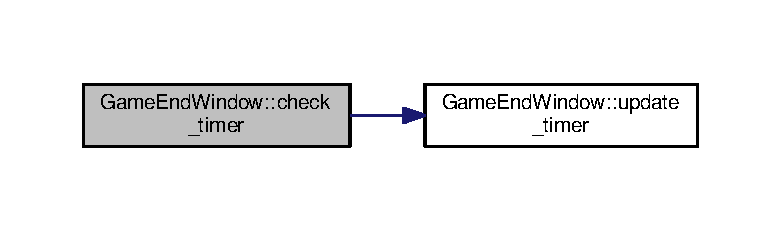
\includegraphics[width=350pt]{classGameEndWindow_a00ec6d032219c692a678b7ddac55a3b3_cgraph}
\end{center}
\end{figure}




Граф вызова функции\+:\nopagebreak
\begin{figure}[H]
\begin{center}
\leavevmode
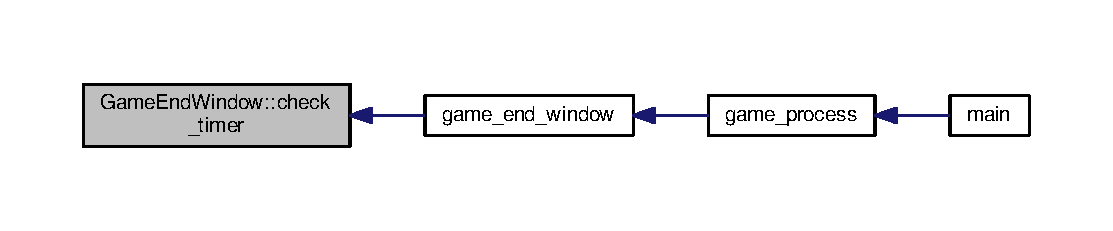
\includegraphics[width=350pt]{classGameEndWindow_a00ec6d032219c692a678b7ddac55a3b3_icgraph}
\end{center}
\end{figure}


\index{Game\+End\+Window@{Game\+End\+Window}!set\+Description@{set\+Description}}
\index{set\+Description@{set\+Description}!Game\+End\+Window@{Game\+End\+Window}}
\subsubsection[{\texorpdfstring{set\+Description(bool flag)}{setDescription(bool flag)}}]{\setlength{\rightskip}{0pt plus 5cm}void Game\+End\+Window\+::set\+Description (
\begin{DoxyParamCaption}
\item[{bool}]{flag}
\end{DoxyParamCaption}
)\hspace{0.3cm}{\ttfamily [inline]}}\hypertarget{classGameEndWindow_a2f5dcaf5df932f64323d14f58b5649e6}{}\label{classGameEndWindow_a2f5dcaf5df932f64323d14f58b5649e6}


Граф вызова функции\+:\nopagebreak
\begin{figure}[H]
\begin{center}
\leavevmode
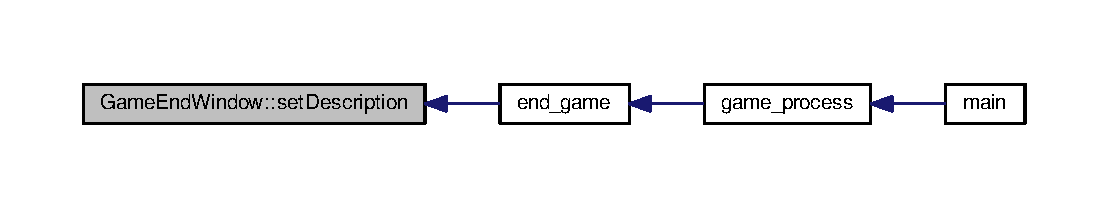
\includegraphics[width=350pt]{classGameEndWindow_a2f5dcaf5df932f64323d14f58b5649e6_icgraph}
\end{center}
\end{figure}


\index{Game\+End\+Window@{Game\+End\+Window}!update\+\_\+timer@{update\+\_\+timer}}
\index{update\+\_\+timer@{update\+\_\+timer}!Game\+End\+Window@{Game\+End\+Window}}
\subsubsection[{\texorpdfstring{update\+\_\+timer()}{update_timer()}}]{\setlength{\rightskip}{0pt plus 5cm}void Game\+End\+Window\+::update\+\_\+timer (
\begin{DoxyParamCaption}
{}
\end{DoxyParamCaption}
)\hspace{0.3cm}{\ttfamily [inline]}}\hypertarget{classGameEndWindow_a91d7d99ae0dac923a1bf764f7b5d996f}{}\label{classGameEndWindow_a91d7d99ae0dac923a1bf764f7b5d996f}


Граф вызова функции\+:\nopagebreak
\begin{figure}[H]
\begin{center}
\leavevmode
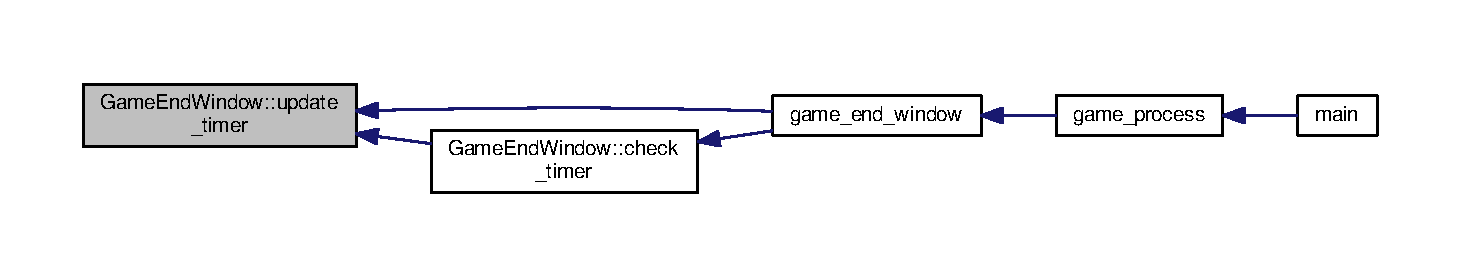
\includegraphics[width=350pt]{classGameEndWindow_a91d7d99ae0dac923a1bf764f7b5d996f_icgraph}
\end{center}
\end{figure}




\subsection{Поля}
\index{Game\+End\+Window@{Game\+End\+Window}!description@{description}}
\index{description@{description}!Game\+End\+Window@{Game\+End\+Window}}
\subsubsection[{\texorpdfstring{description}{description}}]{\setlength{\rightskip}{0pt plus 5cm}sf\+::\+Text Game\+End\+Window\+::description}\hypertarget{classGameEndWindow_ab29a8ae98c80ff3facba1c9f58f57ed1}{}\label{classGameEndWindow_ab29a8ae98c80ff3facba1c9f58f57ed1}
\index{Game\+End\+Window@{Game\+End\+Window}!h@{h}}
\index{h@{h}!Game\+End\+Window@{Game\+End\+Window}}
\subsubsection[{\texorpdfstring{h}{h}}]{\setlength{\rightskip}{0pt plus 5cm}int Game\+End\+Window\+::h}\hypertarget{classGameEndWindow_adf2232ddacea4f327e8b1315633f4e4b}{}\label{classGameEndWindow_adf2232ddacea4f327e8b1315633f4e4b}
\index{Game\+End\+Window@{Game\+End\+Window}!seconds\+Till\+Exit@{seconds\+Till\+Exit}}
\index{seconds\+Till\+Exit@{seconds\+Till\+Exit}!Game\+End\+Window@{Game\+End\+Window}}
\subsubsection[{\texorpdfstring{seconds\+Till\+Exit}{secondsTillExit}}]{\setlength{\rightskip}{0pt plus 5cm}int Game\+End\+Window\+::seconds\+Till\+Exit}\hypertarget{classGameEndWindow_a7705716c485ae134468ec5cc3e92812d}{}\label{classGameEndWindow_a7705716c485ae134468ec5cc3e92812d}
\index{Game\+End\+Window@{Game\+End\+Window}!sprite@{sprite}}
\index{sprite@{sprite}!Game\+End\+Window@{Game\+End\+Window}}
\subsubsection[{\texorpdfstring{sprite}{sprite}}]{\setlength{\rightskip}{0pt plus 5cm}sf\+::\+Sprite Game\+End\+Window\+::sprite}\hypertarget{classGameEndWindow_ae1cfd12474c38f65885885c05d3f45da}{}\label{classGameEndWindow_ae1cfd12474c38f65885885c05d3f45da}
\index{Game\+End\+Window@{Game\+End\+Window}!timer@{timer}}
\index{timer@{timer}!Game\+End\+Window@{Game\+End\+Window}}
\subsubsection[{\texorpdfstring{timer}{timer}}]{\setlength{\rightskip}{0pt plus 5cm}sf\+::\+Text Game\+End\+Window\+::timer}\hypertarget{classGameEndWindow_a2cda6ea6738d35480ca4ede7fd494fa9}{}\label{classGameEndWindow_a2cda6ea6738d35480ca4ede7fd494fa9}
\index{Game\+End\+Window@{Game\+End\+Window}!w@{w}}
\index{w@{w}!Game\+End\+Window@{Game\+End\+Window}}
\subsubsection[{\texorpdfstring{w}{w}}]{\setlength{\rightskip}{0pt plus 5cm}int Game\+End\+Window\+::w}\hypertarget{classGameEndWindow_aec3d8eedb5288ddb2a218d8e2eb0a3b1}{}\label{classGameEndWindow_aec3d8eedb5288ddb2a218d8e2eb0a3b1}

\hypertarget{classGameObject}{}\section{Класс Game\+Object}
\label{classGameObject}\index{Game\+Object@{Game\+Object}}


Параметры игровых объектов  




{\ttfamily \#include $<$game\+\_\+objects.\+h$>$}



Граф связей класса Game\+Object\+:\nopagebreak
\begin{figure}[H]
\begin{center}
\leavevmode
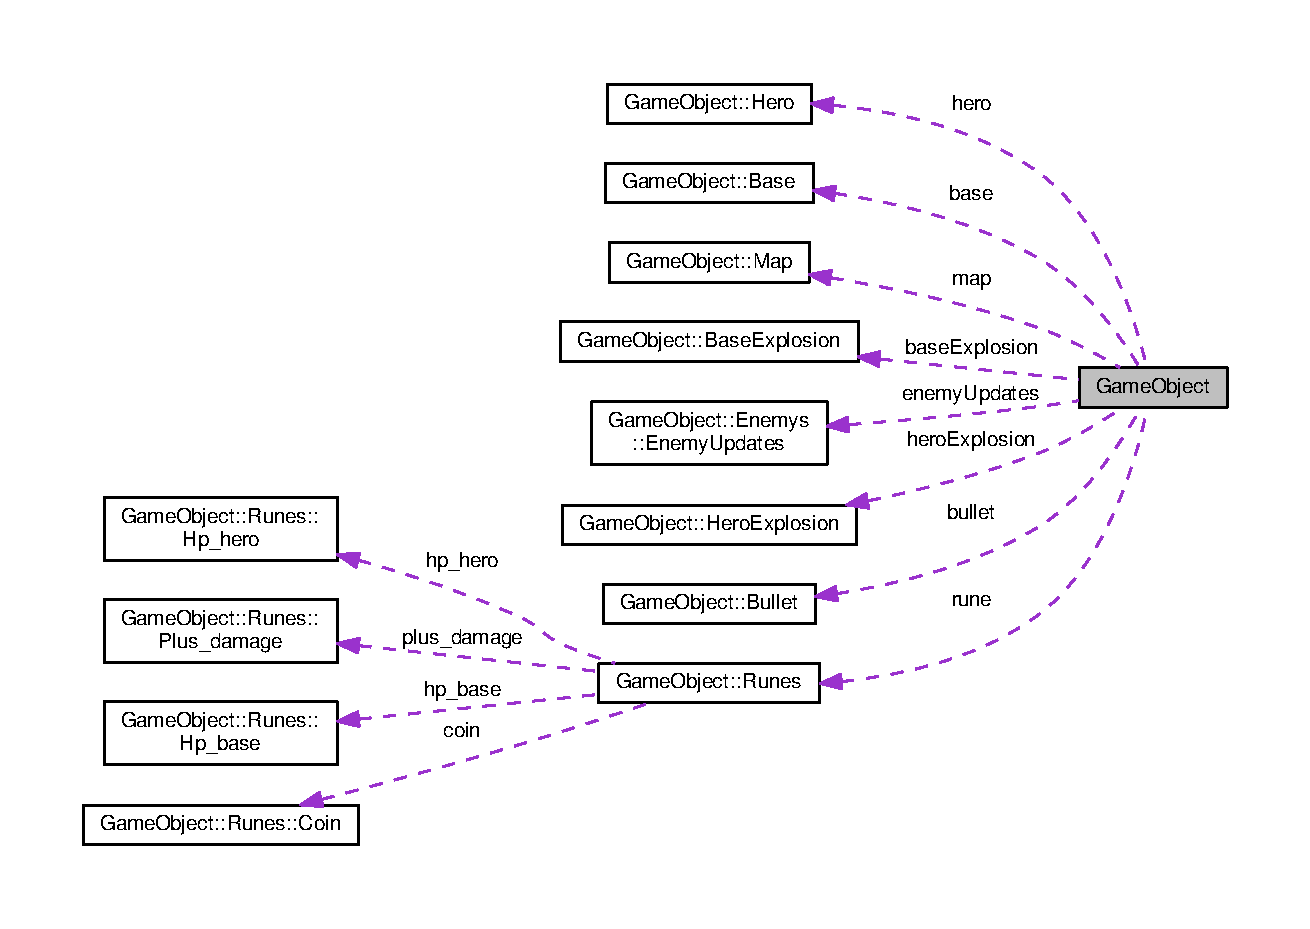
\includegraphics[width=350pt]{classGameObject__coll__graph}
\end{center}
\end{figure}
\subsection*{Структуры данных}
\begin{DoxyCompactItemize}
\item 
class \hyperlink{classGameObject_1_1Base}{Base}
\begin{DoxyCompactList}\small\item\em The \hyperlink{classGameObject_1_1Base}{Base} class. \end{DoxyCompactList}\item 
class \hyperlink{classGameObject_1_1BaseExplosion}{Base\+Explosion}
\begin{DoxyCompactList}\small\item\em The \hyperlink{classGameObject_1_1BaseExplosion}{Base\+Explosion} class. \end{DoxyCompactList}\item 
class \hyperlink{classGameObject_1_1Bullet}{Bullet}
\begin{DoxyCompactList}\small\item\em The \hyperlink{classGameObject_1_1Bullet}{Bullet} class. \end{DoxyCompactList}\item 
class \hyperlink{classGameObject_1_1Enemys}{Enemys}
\begin{DoxyCompactList}\small\item\em The \hyperlink{classGameObject_1_1Enemys}{Enemys} class. \end{DoxyCompactList}\item 
class \hyperlink{classGameObject_1_1Hero}{Hero}
\begin{DoxyCompactList}\small\item\em The \hyperlink{classGameObject_1_1Hero}{Hero} class. \end{DoxyCompactList}\item 
class \hyperlink{classGameObject_1_1HeroExplosion}{Hero\+Explosion}
\begin{DoxyCompactList}\small\item\em The \hyperlink{classGameObject_1_1HeroExplosion}{Hero\+Explosion} class. \end{DoxyCompactList}\item 
class \hyperlink{classGameObject_1_1Map}{Map}
\item 
class \hyperlink{classGameObject_1_1Runes}{Runes}
\begin{DoxyCompactList}\small\item\em The \hyperlink{classGameObject_1_1Runes}{Runes} class. \end{DoxyCompactList}\end{DoxyCompactItemize}
\subsection*{Поля данных}
\begin{DoxyCompactItemize}
\item 
\hyperlink{classGameObject_1_1Map}{Map} \hyperlink{classGameObject_a49b8b56419192fd29243f4ae9ad8c7f3}{map}
\item 
\hyperlink{classGameObject_1_1Base}{Base} \hyperlink{classGameObject_a0d441ea1c04535a1bcfcf0dacd3e46b6}{base}
\item 
\hyperlink{classGameObject_1_1BaseExplosion}{Base\+Explosion} \hyperlink{classGameObject_a03d9b8baaf2b58f0074fe183f4843379}{base\+Explosion}
\item 
\hyperlink{classGameObject_1_1Hero}{Hero} \hyperlink{classGameObject_a492285ce87e02288a1d532f5c83ff773}{hero}
\item 
\hyperlink{classGameObject_1_1HeroExplosion}{Hero\+Explosion} \hyperlink{classGameObject_a3dd518a4cbc7316edf2a4d43efa3dd52}{hero\+Explosion}
\item 
\hyperlink{classGameObject_1_1Runes}{Runes} \hyperlink{classGameObject_aef75ff75d6d246e532f47f54b6fac398}{rune}
\item 
\hyperlink{classGameObject_1_1Bullet}{Bullet} \hyperlink{classGameObject_abfec990ef1d0b3124c838ee9b6357948}{bullet}
\item 
std\+::vector$<$ \hyperlink{classGameObject_1_1Bullet}{Bullet} $>$ \hyperlink{classGameObject_a6c4f71551f2ab511cca56814f3678a11}{bullets}
\item 
\hyperlink{classGameObject_1_1Enemys_1_1EnemyUpdates}{Enemys\+::\+Enemy\+Updates} \hyperlink{classGameObject_a1be22120f03e9c3332dbd74ecb57d8f5}{enemy\+Updates}
\item 
std\+::vector$<$ \hyperlink{classGameObject_1_1Enemys_1_1EnemyTemlate}{Enemys\+::\+Enemy\+Temlate} $>$ \hyperlink{classGameObject_a9ef32e6a46460a1db1d6005eb8a12cdd}{enemy}
\end{DoxyCompactItemize}


\subsection{Подробное описание}
Параметры игровых объектов 

\begin{DoxySeeAlso}{См. также}
\hyperlink{classGameObject_1_1Hero}{Hero}, \hyperlink{classGameObject_1_1Runes}{Runes}, \hyperlink{classGameObject_1_1Enemys}{Enemys}, \hyperlink{classGameObject_1_1Base}{Base} 
\end{DoxySeeAlso}


\subsection{Поля}
\index{Game\+Object@{Game\+Object}!base@{base}}
\index{base@{base}!Game\+Object@{Game\+Object}}
\subsubsection[{\texorpdfstring{base}{base}}]{\setlength{\rightskip}{0pt plus 5cm}{\bf Base} Game\+Object\+::base}\hypertarget{classGameObject_a0d441ea1c04535a1bcfcf0dacd3e46b6}{}\label{classGameObject_a0d441ea1c04535a1bcfcf0dacd3e46b6}
\index{Game\+Object@{Game\+Object}!base\+Explosion@{base\+Explosion}}
\index{base\+Explosion@{base\+Explosion}!Game\+Object@{Game\+Object}}
\subsubsection[{\texorpdfstring{base\+Explosion}{baseExplosion}}]{\setlength{\rightskip}{0pt plus 5cm}{\bf Base\+Explosion} Game\+Object\+::base\+Explosion}\hypertarget{classGameObject_a03d9b8baaf2b58f0074fe183f4843379}{}\label{classGameObject_a03d9b8baaf2b58f0074fe183f4843379}
\index{Game\+Object@{Game\+Object}!bullet@{bullet}}
\index{bullet@{bullet}!Game\+Object@{Game\+Object}}
\subsubsection[{\texorpdfstring{bullet}{bullet}}]{\setlength{\rightskip}{0pt plus 5cm}{\bf Bullet} Game\+Object\+::bullet}\hypertarget{classGameObject_abfec990ef1d0b3124c838ee9b6357948}{}\label{classGameObject_abfec990ef1d0b3124c838ee9b6357948}
\index{Game\+Object@{Game\+Object}!bullets@{bullets}}
\index{bullets@{bullets}!Game\+Object@{Game\+Object}}
\subsubsection[{\texorpdfstring{bullets}{bullets}}]{\setlength{\rightskip}{0pt plus 5cm}std\+::vector$<${\bf Bullet}$>$ Game\+Object\+::bullets}\hypertarget{classGameObject_a6c4f71551f2ab511cca56814f3678a11}{}\label{classGameObject_a6c4f71551f2ab511cca56814f3678a11}
\index{Game\+Object@{Game\+Object}!enemy@{enemy}}
\index{enemy@{enemy}!Game\+Object@{Game\+Object}}
\subsubsection[{\texorpdfstring{enemy}{enemy}}]{\setlength{\rightskip}{0pt plus 5cm}std\+::vector$<${\bf Enemys\+::\+Enemy\+Temlate}$>$ Game\+Object\+::enemy}\hypertarget{classGameObject_a9ef32e6a46460a1db1d6005eb8a12cdd}{}\label{classGameObject_a9ef32e6a46460a1db1d6005eb8a12cdd}
\index{Game\+Object@{Game\+Object}!enemy\+Updates@{enemy\+Updates}}
\index{enemy\+Updates@{enemy\+Updates}!Game\+Object@{Game\+Object}}
\subsubsection[{\texorpdfstring{enemy\+Updates}{enemyUpdates}}]{\setlength{\rightskip}{0pt plus 5cm}{\bf Enemys\+::\+Enemy\+Updates} Game\+Object\+::enemy\+Updates}\hypertarget{classGameObject_a1be22120f03e9c3332dbd74ecb57d8f5}{}\label{classGameObject_a1be22120f03e9c3332dbd74ecb57d8f5}
\index{Game\+Object@{Game\+Object}!hero@{hero}}
\index{hero@{hero}!Game\+Object@{Game\+Object}}
\subsubsection[{\texorpdfstring{hero}{hero}}]{\setlength{\rightskip}{0pt plus 5cm}{\bf Hero} Game\+Object\+::hero}\hypertarget{classGameObject_a492285ce87e02288a1d532f5c83ff773}{}\label{classGameObject_a492285ce87e02288a1d532f5c83ff773}
\index{Game\+Object@{Game\+Object}!hero\+Explosion@{hero\+Explosion}}
\index{hero\+Explosion@{hero\+Explosion}!Game\+Object@{Game\+Object}}
\subsubsection[{\texorpdfstring{hero\+Explosion}{heroExplosion}}]{\setlength{\rightskip}{0pt plus 5cm}{\bf Hero\+Explosion} Game\+Object\+::hero\+Explosion}\hypertarget{classGameObject_a3dd518a4cbc7316edf2a4d43efa3dd52}{}\label{classGameObject_a3dd518a4cbc7316edf2a4d43efa3dd52}
\index{Game\+Object@{Game\+Object}!map@{map}}
\index{map@{map}!Game\+Object@{Game\+Object}}
\subsubsection[{\texorpdfstring{map}{map}}]{\setlength{\rightskip}{0pt plus 5cm}{\bf Map} Game\+Object\+::map}\hypertarget{classGameObject_a49b8b56419192fd29243f4ae9ad8c7f3}{}\label{classGameObject_a49b8b56419192fd29243f4ae9ad8c7f3}
\index{Game\+Object@{Game\+Object}!rune@{rune}}
\index{rune@{rune}!Game\+Object@{Game\+Object}}
\subsubsection[{\texorpdfstring{rune}{rune}}]{\setlength{\rightskip}{0pt plus 5cm}{\bf Runes} Game\+Object\+::rune}\hypertarget{classGameObject_aef75ff75d6d246e532f47f54b6fac398}{}\label{classGameObject_aef75ff75d6d246e532f47f54b6fac398}

\hypertarget{classGameObject_1_1Hero}{}\section{Класс Game\+Object\+:\+:Hero}
\label{classGameObject_1_1Hero}\index{Game\+Object\+::\+Hero@{Game\+Object\+::\+Hero}}


The \hyperlink{classGameObject_1_1Hero}{Hero} class.  




{\ttfamily \#include $<$game\+\_\+objects.\+h$>$}

\subsection*{Открытые члены}
\begin{DoxyCompactItemize}
\item 
\hyperlink{classGameObject_1_1Hero_a4489910b28781db349f14ec1c84c0861}{Hero} ()
\end{DoxyCompactItemize}
\subsection*{Поля данных}
\begin{DoxyCompactItemize}
\item 
sf\+::\+Sprite \hyperlink{classGameObject_1_1Hero_aba95da2b9327e20c6031c4159d7ca017}{sprite}
\item 
float \hyperlink{classGameObject_1_1Hero_a19fdfb7b36ab53173913698cc14feae0}{h}
\item 
float \hyperlink{classGameObject_1_1Hero_ac735e21149b7b6e405e21e103a058f27}{w}
\item 
float \hyperlink{classGameObject_1_1Hero_ab9aa6c935fe527672dbda1a9c026aecd}{speed}
\item 
int \hyperlink{classGameObject_1_1Hero_a536db911ab73df15c716ed808f453f10}{health}
\item 
bool \hyperlink{classGameObject_1_1Hero_af61f8b4ea25b9b12bebfd444bc125799}{live}
\item 
int \hyperlink{classGameObject_1_1Hero_a3c46e9c476100f2d29d22bdf6364a303}{gun\+\_\+direction}
\item 
float \hyperlink{classGameObject_1_1Hero_a4a085321b5cffd9dc388503ee1deafb7}{pos\+\_\+gun\+\_\+dir\+\_\+x}
\item 
float \hyperlink{classGameObject_1_1Hero_af6fd4f63cfa0f1177e1ffa1cfae8881d}{pos\+\_\+gun\+\_\+dir\+\_\+y}
\end{DoxyCompactItemize}


\subsection{Подробное описание}
The \hyperlink{classGameObject_1_1Hero}{Hero} class. 

\subsection{Конструктор(ы)}
\index{Game\+Object\+::\+Hero@{Game\+Object\+::\+Hero}!Hero@{Hero}}
\index{Hero@{Hero}!Game\+Object\+::\+Hero@{Game\+Object\+::\+Hero}}
\subsubsection[{\texorpdfstring{Hero()}{Hero()}}]{\setlength{\rightskip}{0pt plus 5cm}Game\+Object\+::\+Hero\+::\+Hero (
\begin{DoxyParamCaption}
{}
\end{DoxyParamCaption}
)\hspace{0.3cm}{\ttfamily [inline]}}\hypertarget{classGameObject_1_1Hero_a4489910b28781db349f14ec1c84c0861}{}\label{classGameObject_1_1Hero_a4489910b28781db349f14ec1c84c0861}


\subsection{Поля}
\index{Game\+Object\+::\+Hero@{Game\+Object\+::\+Hero}!gun\+\_\+direction@{gun\+\_\+direction}}
\index{gun\+\_\+direction@{gun\+\_\+direction}!Game\+Object\+::\+Hero@{Game\+Object\+::\+Hero}}
\subsubsection[{\texorpdfstring{gun\+\_\+direction}{gun_direction}}]{\setlength{\rightskip}{0pt plus 5cm}int Game\+Object\+::\+Hero\+::gun\+\_\+direction}\hypertarget{classGameObject_1_1Hero_a3c46e9c476100f2d29d22bdf6364a303}{}\label{classGameObject_1_1Hero_a3c46e9c476100f2d29d22bdf6364a303}
\index{Game\+Object\+::\+Hero@{Game\+Object\+::\+Hero}!h@{h}}
\index{h@{h}!Game\+Object\+::\+Hero@{Game\+Object\+::\+Hero}}
\subsubsection[{\texorpdfstring{h}{h}}]{\setlength{\rightskip}{0pt plus 5cm}float Game\+Object\+::\+Hero\+::h}\hypertarget{classGameObject_1_1Hero_a19fdfb7b36ab53173913698cc14feae0}{}\label{classGameObject_1_1Hero_a19fdfb7b36ab53173913698cc14feae0}
\index{Game\+Object\+::\+Hero@{Game\+Object\+::\+Hero}!health@{health}}
\index{health@{health}!Game\+Object\+::\+Hero@{Game\+Object\+::\+Hero}}
\subsubsection[{\texorpdfstring{health}{health}}]{\setlength{\rightskip}{0pt plus 5cm}int Game\+Object\+::\+Hero\+::health}\hypertarget{classGameObject_1_1Hero_a536db911ab73df15c716ed808f453f10}{}\label{classGameObject_1_1Hero_a536db911ab73df15c716ed808f453f10}
\index{Game\+Object\+::\+Hero@{Game\+Object\+::\+Hero}!live@{live}}
\index{live@{live}!Game\+Object\+::\+Hero@{Game\+Object\+::\+Hero}}
\subsubsection[{\texorpdfstring{live}{live}}]{\setlength{\rightskip}{0pt plus 5cm}bool Game\+Object\+::\+Hero\+::live}\hypertarget{classGameObject_1_1Hero_af61f8b4ea25b9b12bebfd444bc125799}{}\label{classGameObject_1_1Hero_af61f8b4ea25b9b12bebfd444bc125799}
\index{Game\+Object\+::\+Hero@{Game\+Object\+::\+Hero}!pos\+\_\+gun\+\_\+dir\+\_\+x@{pos\+\_\+gun\+\_\+dir\+\_\+x}}
\index{pos\+\_\+gun\+\_\+dir\+\_\+x@{pos\+\_\+gun\+\_\+dir\+\_\+x}!Game\+Object\+::\+Hero@{Game\+Object\+::\+Hero}}
\subsubsection[{\texorpdfstring{pos\+\_\+gun\+\_\+dir\+\_\+x}{pos_gun_dir_x}}]{\setlength{\rightskip}{0pt plus 5cm}float Game\+Object\+::\+Hero\+::pos\+\_\+gun\+\_\+dir\+\_\+x}\hypertarget{classGameObject_1_1Hero_a4a085321b5cffd9dc388503ee1deafb7}{}\label{classGameObject_1_1Hero_a4a085321b5cffd9dc388503ee1deafb7}
\index{Game\+Object\+::\+Hero@{Game\+Object\+::\+Hero}!pos\+\_\+gun\+\_\+dir\+\_\+y@{pos\+\_\+gun\+\_\+dir\+\_\+y}}
\index{pos\+\_\+gun\+\_\+dir\+\_\+y@{pos\+\_\+gun\+\_\+dir\+\_\+y}!Game\+Object\+::\+Hero@{Game\+Object\+::\+Hero}}
\subsubsection[{\texorpdfstring{pos\+\_\+gun\+\_\+dir\+\_\+y}{pos_gun_dir_y}}]{\setlength{\rightskip}{0pt plus 5cm}float Game\+Object\+::\+Hero\+::pos\+\_\+gun\+\_\+dir\+\_\+y}\hypertarget{classGameObject_1_1Hero_af6fd4f63cfa0f1177e1ffa1cfae8881d}{}\label{classGameObject_1_1Hero_af6fd4f63cfa0f1177e1ffa1cfae8881d}
\index{Game\+Object\+::\+Hero@{Game\+Object\+::\+Hero}!speed@{speed}}
\index{speed@{speed}!Game\+Object\+::\+Hero@{Game\+Object\+::\+Hero}}
\subsubsection[{\texorpdfstring{speed}{speed}}]{\setlength{\rightskip}{0pt plus 5cm}float Game\+Object\+::\+Hero\+::speed}\hypertarget{classGameObject_1_1Hero_ab9aa6c935fe527672dbda1a9c026aecd}{}\label{classGameObject_1_1Hero_ab9aa6c935fe527672dbda1a9c026aecd}
\index{Game\+Object\+::\+Hero@{Game\+Object\+::\+Hero}!sprite@{sprite}}
\index{sprite@{sprite}!Game\+Object\+::\+Hero@{Game\+Object\+::\+Hero}}
\subsubsection[{\texorpdfstring{sprite}{sprite}}]{\setlength{\rightskip}{0pt plus 5cm}sf\+::\+Sprite Game\+Object\+::\+Hero\+::sprite}\hypertarget{classGameObject_1_1Hero_aba95da2b9327e20c6031c4159d7ca017}{}\label{classGameObject_1_1Hero_aba95da2b9327e20c6031c4159d7ca017}
\index{Game\+Object\+::\+Hero@{Game\+Object\+::\+Hero}!w@{w}}
\index{w@{w}!Game\+Object\+::\+Hero@{Game\+Object\+::\+Hero}}
\subsubsection[{\texorpdfstring{w}{w}}]{\setlength{\rightskip}{0pt plus 5cm}float Game\+Object\+::\+Hero\+::w}\hypertarget{classGameObject_1_1Hero_ac735e21149b7b6e405e21e103a058f27}{}\label{classGameObject_1_1Hero_ac735e21149b7b6e405e21e103a058f27}

\hypertarget{classGameObject_1_1HeroExplosion}{}\section{Класс Game\+Object\+:\+:Hero\+Explosion}
\label{classGameObject_1_1HeroExplosion}\index{Game\+Object\+::\+Hero\+Explosion@{Game\+Object\+::\+Hero\+Explosion}}


The \hyperlink{classGameObject_1_1HeroExplosion}{Hero\+Explosion} class.  




{\ttfamily \#include $<$game\+\_\+objects.\+h$>$}

\subsection*{Открытые члены}
\begin{DoxyCompactItemize}
\item 
\hyperlink{classGameObject_1_1HeroExplosion_a6bbe6fd284863bcf70b0e4447d8f46c1}{Hero\+Explosion} ()
\item 
bool \hyperlink{classGameObject_1_1HeroExplosion_ac5fa2bfc1bdd8179ad5f113d81e19252}{update\+Frame} ()
\end{DoxyCompactItemize}
\subsection*{Поля данных}
\begin{DoxyCompactItemize}
\item 
sf\+::\+Sprite \hyperlink{classGameObject_1_1HeroExplosion_a6d55438bf1ecf9ced768fa677ebe646d}{sprite}
\item 
float \hyperlink{classGameObject_1_1HeroExplosion_afdb47a4793449f3f75d657535ea6be2c}{w}
\item 
float \hyperlink{classGameObject_1_1HeroExplosion_a3934725c63657743d0ee6d08030a36a1}{h}
\item 
float \hyperlink{classGameObject_1_1HeroExplosion_a9484619a70aa340b7960984067053225}{colomn}
\end{DoxyCompactItemize}


\subsection{Подробное описание}
The \hyperlink{classGameObject_1_1HeroExplosion}{Hero\+Explosion} class. 

\subsection{Конструктор(ы)}
\index{Game\+Object\+::\+Hero\+Explosion@{Game\+Object\+::\+Hero\+Explosion}!Hero\+Explosion@{Hero\+Explosion}}
\index{Hero\+Explosion@{Hero\+Explosion}!Game\+Object\+::\+Hero\+Explosion@{Game\+Object\+::\+Hero\+Explosion}}
\subsubsection[{\texorpdfstring{Hero\+Explosion()}{HeroExplosion()}}]{\setlength{\rightskip}{0pt plus 5cm}Game\+Object\+::\+Hero\+Explosion\+::\+Hero\+Explosion (
\begin{DoxyParamCaption}
{}
\end{DoxyParamCaption}
)\hspace{0.3cm}{\ttfamily [inline]}}\hypertarget{classGameObject_1_1HeroExplosion_a6bbe6fd284863bcf70b0e4447d8f46c1}{}\label{classGameObject_1_1HeroExplosion_a6bbe6fd284863bcf70b0e4447d8f46c1}


\subsection{Методы}
\index{Game\+Object\+::\+Hero\+Explosion@{Game\+Object\+::\+Hero\+Explosion}!update\+Frame@{update\+Frame}}
\index{update\+Frame@{update\+Frame}!Game\+Object\+::\+Hero\+Explosion@{Game\+Object\+::\+Hero\+Explosion}}
\subsubsection[{\texorpdfstring{update\+Frame()}{updateFrame()}}]{\setlength{\rightskip}{0pt plus 5cm}bool Game\+Object\+::\+Hero\+Explosion\+::update\+Frame (
\begin{DoxyParamCaption}
{}
\end{DoxyParamCaption}
)\hspace{0.3cm}{\ttfamily [inline]}}\hypertarget{classGameObject_1_1HeroExplosion_ac5fa2bfc1bdd8179ad5f113d81e19252}{}\label{classGameObject_1_1HeroExplosion_ac5fa2bfc1bdd8179ad5f113d81e19252}


\subsection{Поля}
\index{Game\+Object\+::\+Hero\+Explosion@{Game\+Object\+::\+Hero\+Explosion}!colomn@{colomn}}
\index{colomn@{colomn}!Game\+Object\+::\+Hero\+Explosion@{Game\+Object\+::\+Hero\+Explosion}}
\subsubsection[{\texorpdfstring{colomn}{colomn}}]{\setlength{\rightskip}{0pt plus 5cm}float Game\+Object\+::\+Hero\+Explosion\+::colomn}\hypertarget{classGameObject_1_1HeroExplosion_a9484619a70aa340b7960984067053225}{}\label{classGameObject_1_1HeroExplosion_a9484619a70aa340b7960984067053225}
\index{Game\+Object\+::\+Hero\+Explosion@{Game\+Object\+::\+Hero\+Explosion}!h@{h}}
\index{h@{h}!Game\+Object\+::\+Hero\+Explosion@{Game\+Object\+::\+Hero\+Explosion}}
\subsubsection[{\texorpdfstring{h}{h}}]{\setlength{\rightskip}{0pt plus 5cm}float Game\+Object\+::\+Hero\+Explosion\+::h}\hypertarget{classGameObject_1_1HeroExplosion_a3934725c63657743d0ee6d08030a36a1}{}\label{classGameObject_1_1HeroExplosion_a3934725c63657743d0ee6d08030a36a1}
\index{Game\+Object\+::\+Hero\+Explosion@{Game\+Object\+::\+Hero\+Explosion}!sprite@{sprite}}
\index{sprite@{sprite}!Game\+Object\+::\+Hero\+Explosion@{Game\+Object\+::\+Hero\+Explosion}}
\subsubsection[{\texorpdfstring{sprite}{sprite}}]{\setlength{\rightskip}{0pt plus 5cm}sf\+::\+Sprite Game\+Object\+::\+Hero\+Explosion\+::sprite}\hypertarget{classGameObject_1_1HeroExplosion_a6d55438bf1ecf9ced768fa677ebe646d}{}\label{classGameObject_1_1HeroExplosion_a6d55438bf1ecf9ced768fa677ebe646d}
\index{Game\+Object\+::\+Hero\+Explosion@{Game\+Object\+::\+Hero\+Explosion}!w@{w}}
\index{w@{w}!Game\+Object\+::\+Hero\+Explosion@{Game\+Object\+::\+Hero\+Explosion}}
\subsubsection[{\texorpdfstring{w}{w}}]{\setlength{\rightskip}{0pt plus 5cm}float Game\+Object\+::\+Hero\+Explosion\+::w}\hypertarget{classGameObject_1_1HeroExplosion_afdb47a4793449f3f75d657535ea6be2c}{}\label{classGameObject_1_1HeroExplosion_afdb47a4793449f3f75d657535ea6be2c}

\hypertarget{classGameObject_1_1Runes_1_1Hp__base}{}\section{Класс Game\+Object\+:\+:Runes\+:\+:Hp\+\_\+base}
\label{classGameObject_1_1Runes_1_1Hp__base}\index{Game\+Object\+::\+Runes\+::\+Hp\+\_\+base@{Game\+Object\+::\+Runes\+::\+Hp\+\_\+base}}


The \hyperlink{classGameObject_1_1Runes_1_1Hp__base}{Hp\+\_\+base} class.  




{\ttfamily \#include $<$game\+\_\+objects.\+h$>$}

\subsection*{Открытые члены}
\begin{DoxyCompactItemize}
\item 
\hyperlink{classGameObject_1_1Runes_1_1Hp__base_af2eaac200783be6060f53e2fc1dd317a}{Hp\+\_\+base} ()
\end{DoxyCompactItemize}
\subsection*{Поля данных}
\begin{DoxyCompactItemize}
\item 
sf\+::\+Sprite \hyperlink{classGameObject_1_1Runes_1_1Hp__base_aaee646db3a5ea04462ae77a08c475d16}{sprite}
\item 
float \hyperlink{classGameObject_1_1Runes_1_1Hp__base_a57360af5bfe84e33fddfc5c41a7c9c91}{w}
\item 
float \hyperlink{classGameObject_1_1Runes_1_1Hp__base_abeffb8fe7917662111a77cf70c25fae5}{h}
\item 
float \hyperlink{classGameObject_1_1Runes_1_1Hp__base_a6cd250a0e85ad0449365f33d452c6e28}{frames}
\item 
float \hyperlink{classGameObject_1_1Runes_1_1Hp__base_a6019c25a6c56252b3a059d537b80b798}{current\+\_\+frame}
\item 
int \hyperlink{classGameObject_1_1Runes_1_1Hp__base_ae6d1b0b8a2aa0ae71e7c26fff65b263c}{regen\+HP}
\end{DoxyCompactItemize}


\subsection{Подробное описание}
The \hyperlink{classGameObject_1_1Runes_1_1Hp__base}{Hp\+\_\+base} class. 

\subsection{Конструктор(ы)}
\index{Game\+Object\+::\+Runes\+::\+Hp\+\_\+base@{Game\+Object\+::\+Runes\+::\+Hp\+\_\+base}!Hp\+\_\+base@{Hp\+\_\+base}}
\index{Hp\+\_\+base@{Hp\+\_\+base}!Game\+Object\+::\+Runes\+::\+Hp\+\_\+base@{Game\+Object\+::\+Runes\+::\+Hp\+\_\+base}}
\subsubsection[{\texorpdfstring{Hp\+\_\+base()}{Hp_base()}}]{\setlength{\rightskip}{0pt plus 5cm}Game\+Object\+::\+Runes\+::\+Hp\+\_\+base\+::\+Hp\+\_\+base (
\begin{DoxyParamCaption}
{}
\end{DoxyParamCaption}
)\hspace{0.3cm}{\ttfamily [inline]}}\hypertarget{classGameObject_1_1Runes_1_1Hp__base_af2eaac200783be6060f53e2fc1dd317a}{}\label{classGameObject_1_1Runes_1_1Hp__base_af2eaac200783be6060f53e2fc1dd317a}


\subsection{Поля}
\index{Game\+Object\+::\+Runes\+::\+Hp\+\_\+base@{Game\+Object\+::\+Runes\+::\+Hp\+\_\+base}!current\+\_\+frame@{current\+\_\+frame}}
\index{current\+\_\+frame@{current\+\_\+frame}!Game\+Object\+::\+Runes\+::\+Hp\+\_\+base@{Game\+Object\+::\+Runes\+::\+Hp\+\_\+base}}
\subsubsection[{\texorpdfstring{current\+\_\+frame}{current_frame}}]{\setlength{\rightskip}{0pt plus 5cm}float Game\+Object\+::\+Runes\+::\+Hp\+\_\+base\+::current\+\_\+frame}\hypertarget{classGameObject_1_1Runes_1_1Hp__base_a6019c25a6c56252b3a059d537b80b798}{}\label{classGameObject_1_1Runes_1_1Hp__base_a6019c25a6c56252b3a059d537b80b798}
\index{Game\+Object\+::\+Runes\+::\+Hp\+\_\+base@{Game\+Object\+::\+Runes\+::\+Hp\+\_\+base}!frames@{frames}}
\index{frames@{frames}!Game\+Object\+::\+Runes\+::\+Hp\+\_\+base@{Game\+Object\+::\+Runes\+::\+Hp\+\_\+base}}
\subsubsection[{\texorpdfstring{frames}{frames}}]{\setlength{\rightskip}{0pt plus 5cm}float Game\+Object\+::\+Runes\+::\+Hp\+\_\+base\+::frames}\hypertarget{classGameObject_1_1Runes_1_1Hp__base_a6cd250a0e85ad0449365f33d452c6e28}{}\label{classGameObject_1_1Runes_1_1Hp__base_a6cd250a0e85ad0449365f33d452c6e28}
\index{Game\+Object\+::\+Runes\+::\+Hp\+\_\+base@{Game\+Object\+::\+Runes\+::\+Hp\+\_\+base}!h@{h}}
\index{h@{h}!Game\+Object\+::\+Runes\+::\+Hp\+\_\+base@{Game\+Object\+::\+Runes\+::\+Hp\+\_\+base}}
\subsubsection[{\texorpdfstring{h}{h}}]{\setlength{\rightskip}{0pt plus 5cm}float Game\+Object\+::\+Runes\+::\+Hp\+\_\+base\+::h}\hypertarget{classGameObject_1_1Runes_1_1Hp__base_abeffb8fe7917662111a77cf70c25fae5}{}\label{classGameObject_1_1Runes_1_1Hp__base_abeffb8fe7917662111a77cf70c25fae5}
\index{Game\+Object\+::\+Runes\+::\+Hp\+\_\+base@{Game\+Object\+::\+Runes\+::\+Hp\+\_\+base}!regen\+HP@{regen\+HP}}
\index{regen\+HP@{regen\+HP}!Game\+Object\+::\+Runes\+::\+Hp\+\_\+base@{Game\+Object\+::\+Runes\+::\+Hp\+\_\+base}}
\subsubsection[{\texorpdfstring{regen\+HP}{regenHP}}]{\setlength{\rightskip}{0pt plus 5cm}int Game\+Object\+::\+Runes\+::\+Hp\+\_\+base\+::regen\+HP}\hypertarget{classGameObject_1_1Runes_1_1Hp__base_ae6d1b0b8a2aa0ae71e7c26fff65b263c}{}\label{classGameObject_1_1Runes_1_1Hp__base_ae6d1b0b8a2aa0ae71e7c26fff65b263c}
\index{Game\+Object\+::\+Runes\+::\+Hp\+\_\+base@{Game\+Object\+::\+Runes\+::\+Hp\+\_\+base}!sprite@{sprite}}
\index{sprite@{sprite}!Game\+Object\+::\+Runes\+::\+Hp\+\_\+base@{Game\+Object\+::\+Runes\+::\+Hp\+\_\+base}}
\subsubsection[{\texorpdfstring{sprite}{sprite}}]{\setlength{\rightskip}{0pt plus 5cm}sf\+::\+Sprite Game\+Object\+::\+Runes\+::\+Hp\+\_\+base\+::sprite}\hypertarget{classGameObject_1_1Runes_1_1Hp__base_aaee646db3a5ea04462ae77a08c475d16}{}\label{classGameObject_1_1Runes_1_1Hp__base_aaee646db3a5ea04462ae77a08c475d16}
\index{Game\+Object\+::\+Runes\+::\+Hp\+\_\+base@{Game\+Object\+::\+Runes\+::\+Hp\+\_\+base}!w@{w}}
\index{w@{w}!Game\+Object\+::\+Runes\+::\+Hp\+\_\+base@{Game\+Object\+::\+Runes\+::\+Hp\+\_\+base}}
\subsubsection[{\texorpdfstring{w}{w}}]{\setlength{\rightskip}{0pt plus 5cm}float Game\+Object\+::\+Runes\+::\+Hp\+\_\+base\+::w}\hypertarget{classGameObject_1_1Runes_1_1Hp__base_a57360af5bfe84e33fddfc5c41a7c9c91}{}\label{classGameObject_1_1Runes_1_1Hp__base_a57360af5bfe84e33fddfc5c41a7c9c91}

\hypertarget{classGameObject_1_1Runes_1_1Hp__hero}{}\section{Класс Game\+Object\+:\+:Runes\+:\+:Hp\+\_\+hero}
\label{classGameObject_1_1Runes_1_1Hp__hero}\index{Game\+Object\+::\+Runes\+::\+Hp\+\_\+hero@{Game\+Object\+::\+Runes\+::\+Hp\+\_\+hero}}


The \hyperlink{classGameObject_1_1Runes_1_1Hp__hero}{Hp\+\_\+hero} class.  




{\ttfamily \#include $<$game\+\_\+objects.\+h$>$}

\subsection*{Открытые члены}
\begin{DoxyCompactItemize}
\item 
\hyperlink{classGameObject_1_1Runes_1_1Hp__hero_a05e22228414e0343e27562973532359d}{Hp\+\_\+hero} ()
\end{DoxyCompactItemize}
\subsection*{Поля данных}
\begin{DoxyCompactItemize}
\item 
sf\+::\+Sprite \hyperlink{classGameObject_1_1Runes_1_1Hp__hero_ad32b6f46b52b116b6ec935db8b3354cd}{sprite}
\item 
float \hyperlink{classGameObject_1_1Runes_1_1Hp__hero_a52771269c044c6bffb526375ce99e40d}{w}
\item 
float \hyperlink{classGameObject_1_1Runes_1_1Hp__hero_ae8a7c6ed63ded9894eb0dd5e64f4bd6e}{h}
\item 
float \hyperlink{classGameObject_1_1Runes_1_1Hp__hero_a82d8e6e0510f203abe8b567722569b02}{frames}
\item 
float \hyperlink{classGameObject_1_1Runes_1_1Hp__hero_a64ca597b8a89a8462b3b133ab1ef09a9}{current\+\_\+frame}
\item 
int \hyperlink{classGameObject_1_1Runes_1_1Hp__hero_a65e05a2e7adac76e73c3543bfc132395}{regen\+HP}
\end{DoxyCompactItemize}


\subsection{Подробное описание}
The \hyperlink{classGameObject_1_1Runes_1_1Hp__hero}{Hp\+\_\+hero} class. 

\subsection{Конструктор(ы)}
\index{Game\+Object\+::\+Runes\+::\+Hp\+\_\+hero@{Game\+Object\+::\+Runes\+::\+Hp\+\_\+hero}!Hp\+\_\+hero@{Hp\+\_\+hero}}
\index{Hp\+\_\+hero@{Hp\+\_\+hero}!Game\+Object\+::\+Runes\+::\+Hp\+\_\+hero@{Game\+Object\+::\+Runes\+::\+Hp\+\_\+hero}}
\subsubsection[{\texorpdfstring{Hp\+\_\+hero()}{Hp_hero()}}]{\setlength{\rightskip}{0pt plus 5cm}Game\+Object\+::\+Runes\+::\+Hp\+\_\+hero\+::\+Hp\+\_\+hero (
\begin{DoxyParamCaption}
{}
\end{DoxyParamCaption}
)\hspace{0.3cm}{\ttfamily [inline]}}\hypertarget{classGameObject_1_1Runes_1_1Hp__hero_a05e22228414e0343e27562973532359d}{}\label{classGameObject_1_1Runes_1_1Hp__hero_a05e22228414e0343e27562973532359d}


\subsection{Поля}
\index{Game\+Object\+::\+Runes\+::\+Hp\+\_\+hero@{Game\+Object\+::\+Runes\+::\+Hp\+\_\+hero}!current\+\_\+frame@{current\+\_\+frame}}
\index{current\+\_\+frame@{current\+\_\+frame}!Game\+Object\+::\+Runes\+::\+Hp\+\_\+hero@{Game\+Object\+::\+Runes\+::\+Hp\+\_\+hero}}
\subsubsection[{\texorpdfstring{current\+\_\+frame}{current_frame}}]{\setlength{\rightskip}{0pt plus 5cm}float Game\+Object\+::\+Runes\+::\+Hp\+\_\+hero\+::current\+\_\+frame}\hypertarget{classGameObject_1_1Runes_1_1Hp__hero_a64ca597b8a89a8462b3b133ab1ef09a9}{}\label{classGameObject_1_1Runes_1_1Hp__hero_a64ca597b8a89a8462b3b133ab1ef09a9}
\index{Game\+Object\+::\+Runes\+::\+Hp\+\_\+hero@{Game\+Object\+::\+Runes\+::\+Hp\+\_\+hero}!frames@{frames}}
\index{frames@{frames}!Game\+Object\+::\+Runes\+::\+Hp\+\_\+hero@{Game\+Object\+::\+Runes\+::\+Hp\+\_\+hero}}
\subsubsection[{\texorpdfstring{frames}{frames}}]{\setlength{\rightskip}{0pt plus 5cm}float Game\+Object\+::\+Runes\+::\+Hp\+\_\+hero\+::frames}\hypertarget{classGameObject_1_1Runes_1_1Hp__hero_a82d8e6e0510f203abe8b567722569b02}{}\label{classGameObject_1_1Runes_1_1Hp__hero_a82d8e6e0510f203abe8b567722569b02}
\index{Game\+Object\+::\+Runes\+::\+Hp\+\_\+hero@{Game\+Object\+::\+Runes\+::\+Hp\+\_\+hero}!h@{h}}
\index{h@{h}!Game\+Object\+::\+Runes\+::\+Hp\+\_\+hero@{Game\+Object\+::\+Runes\+::\+Hp\+\_\+hero}}
\subsubsection[{\texorpdfstring{h}{h}}]{\setlength{\rightskip}{0pt plus 5cm}float Game\+Object\+::\+Runes\+::\+Hp\+\_\+hero\+::h}\hypertarget{classGameObject_1_1Runes_1_1Hp__hero_ae8a7c6ed63ded9894eb0dd5e64f4bd6e}{}\label{classGameObject_1_1Runes_1_1Hp__hero_ae8a7c6ed63ded9894eb0dd5e64f4bd6e}
\index{Game\+Object\+::\+Runes\+::\+Hp\+\_\+hero@{Game\+Object\+::\+Runes\+::\+Hp\+\_\+hero}!regen\+HP@{regen\+HP}}
\index{regen\+HP@{regen\+HP}!Game\+Object\+::\+Runes\+::\+Hp\+\_\+hero@{Game\+Object\+::\+Runes\+::\+Hp\+\_\+hero}}
\subsubsection[{\texorpdfstring{regen\+HP}{regenHP}}]{\setlength{\rightskip}{0pt plus 5cm}int Game\+Object\+::\+Runes\+::\+Hp\+\_\+hero\+::regen\+HP}\hypertarget{classGameObject_1_1Runes_1_1Hp__hero_a65e05a2e7adac76e73c3543bfc132395}{}\label{classGameObject_1_1Runes_1_1Hp__hero_a65e05a2e7adac76e73c3543bfc132395}
\index{Game\+Object\+::\+Runes\+::\+Hp\+\_\+hero@{Game\+Object\+::\+Runes\+::\+Hp\+\_\+hero}!sprite@{sprite}}
\index{sprite@{sprite}!Game\+Object\+::\+Runes\+::\+Hp\+\_\+hero@{Game\+Object\+::\+Runes\+::\+Hp\+\_\+hero}}
\subsubsection[{\texorpdfstring{sprite}{sprite}}]{\setlength{\rightskip}{0pt plus 5cm}sf\+::\+Sprite Game\+Object\+::\+Runes\+::\+Hp\+\_\+hero\+::sprite}\hypertarget{classGameObject_1_1Runes_1_1Hp__hero_ad32b6f46b52b116b6ec935db8b3354cd}{}\label{classGameObject_1_1Runes_1_1Hp__hero_ad32b6f46b52b116b6ec935db8b3354cd}
\index{Game\+Object\+::\+Runes\+::\+Hp\+\_\+hero@{Game\+Object\+::\+Runes\+::\+Hp\+\_\+hero}!w@{w}}
\index{w@{w}!Game\+Object\+::\+Runes\+::\+Hp\+\_\+hero@{Game\+Object\+::\+Runes\+::\+Hp\+\_\+hero}}
\subsubsection[{\texorpdfstring{w}{w}}]{\setlength{\rightskip}{0pt plus 5cm}float Game\+Object\+::\+Runes\+::\+Hp\+\_\+hero\+::w}\hypertarget{classGameObject_1_1Runes_1_1Hp__hero_a52771269c044c6bffb526375ce99e40d}{}\label{classGameObject_1_1Runes_1_1Hp__hero_a52771269c044c6bffb526375ce99e40d}

\hypertarget{classGameObject_1_1Map}{}\section{Класс Game\+Object\+:\+:Map}
\label{classGameObject_1_1Map}\index{Game\+Object\+::\+Map@{Game\+Object\+::\+Map}}


{\ttfamily \#include $<$game\+\_\+objects.\+h$>$}

\subsection*{Открытые члены}
\begin{DoxyCompactItemize}
\item 
\hyperlink{classGameObject_1_1Map_a4f4e4d0ea00e889deccad23fc64bb91d}{Map} ()
\end{DoxyCompactItemize}
\subsection*{Поля данных}
\begin{DoxyCompactItemize}
\item 
sf\+::\+Sprite \hyperlink{classGameObject_1_1Map_a94d4bf5f7fb90c227b9a8353914444e1}{sprite}
\item 
float \hyperlink{classGameObject_1_1Map_a3bfda345ad076b54022f9ff5ec372060}{w}
\item 
float \hyperlink{classGameObject_1_1Map_a7671d57b12b426d1b8a7bb9e939d6817}{h}
\end{DoxyCompactItemize}


\subsection{Конструктор(ы)}
\index{Game\+Object\+::\+Map@{Game\+Object\+::\+Map}!Map@{Map}}
\index{Map@{Map}!Game\+Object\+::\+Map@{Game\+Object\+::\+Map}}
\subsubsection[{\texorpdfstring{Map()}{Map()}}]{\setlength{\rightskip}{0pt plus 5cm}Game\+Object\+::\+Map\+::\+Map (
\begin{DoxyParamCaption}
{}
\end{DoxyParamCaption}
)\hspace{0.3cm}{\ttfamily [inline]}}\hypertarget{classGameObject_1_1Map_a4f4e4d0ea00e889deccad23fc64bb91d}{}\label{classGameObject_1_1Map_a4f4e4d0ea00e889deccad23fc64bb91d}


\subsection{Поля}
\index{Game\+Object\+::\+Map@{Game\+Object\+::\+Map}!h@{h}}
\index{h@{h}!Game\+Object\+::\+Map@{Game\+Object\+::\+Map}}
\subsubsection[{\texorpdfstring{h}{h}}]{\setlength{\rightskip}{0pt plus 5cm}float Game\+Object\+::\+Map\+::h}\hypertarget{classGameObject_1_1Map_a7671d57b12b426d1b8a7bb9e939d6817}{}\label{classGameObject_1_1Map_a7671d57b12b426d1b8a7bb9e939d6817}
\index{Game\+Object\+::\+Map@{Game\+Object\+::\+Map}!sprite@{sprite}}
\index{sprite@{sprite}!Game\+Object\+::\+Map@{Game\+Object\+::\+Map}}
\subsubsection[{\texorpdfstring{sprite}{sprite}}]{\setlength{\rightskip}{0pt plus 5cm}sf\+::\+Sprite Game\+Object\+::\+Map\+::sprite}\hypertarget{classGameObject_1_1Map_a94d4bf5f7fb90c227b9a8353914444e1}{}\label{classGameObject_1_1Map_a94d4bf5f7fb90c227b9a8353914444e1}
\index{Game\+Object\+::\+Map@{Game\+Object\+::\+Map}!w@{w}}
\index{w@{w}!Game\+Object\+::\+Map@{Game\+Object\+::\+Map}}
\subsubsection[{\texorpdfstring{w}{w}}]{\setlength{\rightskip}{0pt plus 5cm}float Game\+Object\+::\+Map\+::w}\hypertarget{classGameObject_1_1Map_a3bfda345ad076b54022f9ff5ec372060}{}\label{classGameObject_1_1Map_a3bfda345ad076b54022f9ff5ec372060}

\hypertarget{classMenuBar}{}\section{Класс Menu\+Bar}
\label{classMenuBar}\index{Menu\+Bar@{Menu\+Bar}}


Паметры счётчиков,выводимых в верхней полоске игрового окна  




{\ttfamily \#include $<$menu\+\_\+bar.\+h$>$}

\subsection*{Открытые члены}
\begin{DoxyCompactItemize}
\item 
void \hyperlink{classMenuBar_a8517c956a4d36cdacdcb42989b5dccf3}{incr\+\_\+counter\+\_\+coins} (int value)
\item 
void \hyperlink{classMenuBar_a7a4dec33f791733c1babad22ac06d6e3}{incr\+\_\+counter\+\_\+added\+\_\+damage} (int value)
\item 
void \hyperlink{classMenuBar_ab23d3bd560cb6a83deddad9ca2880c5b}{check\+\_\+for\+\_\+next\+\_\+round} (sf\+::\+Clock \&clock, int add\+To\+Timer, int \&added\+Dmg\+In\+Perct, int \&added\+Hp\+In\+Perct)
\item 
void \hyperlink{classMenuBar_a803dd882281e407e0494d2e5c45962bc}{change\+\_\+round} ()
\item 
\hyperlink{classMenuBar_a76a0ec8b0b4cba2775fa71e1791efc6d}{Menu\+Bar} ()
\end{DoxyCompactItemize}
\subsection*{Поля данных}
\begin{DoxyCompactItemize}
\item 
sf\+::\+Sprite \hyperlink{classMenuBar_a7c9348add51432373a0ac9ba34e0cc4a}{menubarline}
\item 
sf\+::\+Sprite \hyperlink{classMenuBar_a607b5c0461ef7951f3c0476bfd2ff00f}{pause\+Button}
\item 
sf\+::\+Sprite \hyperlink{classMenuBar_a68d781e6301956723cf9826650ad7d2c}{pause\+Button\+Text}
\item 
int \hyperlink{classMenuBar_a3e9680e7db9109858b09c1ade97fd5d4}{w}
\item 
int \hyperlink{classMenuBar_a47f733e89c961de1ff15c2534b2c6f9b}{h}
\item 
sf\+::\+Sprite \hyperlink{classMenuBar_a8ba645ebcb1785788ea4763822fac236}{Pause\+Menu}
\item 
sf\+::\+Sprite \hyperlink{classMenuBar_a985fe3e19ae94063f676bcedab881b21}{Pause\+Menu\+Button\+Exit}
\item 
sf\+::\+Text \hyperlink{classMenuBar_ae9cd84f5d9a3b53d45b27cae6a7c44e6}{Exit\+Text}
\item 
sf\+::\+Sprite \hyperlink{classMenuBar_a85b1a76501dd0d2ab5989a36b18299f2}{Pause\+Menu\+Button\+Continue}
\item 
sf\+::\+Text \hyperlink{classMenuBar_aa01962756e77381b16471f863ed3c9c0}{Continue\+Text}
\item 
sf\+::\+Text \hyperlink{classMenuBar_af2f5d854bc3f91aec40595f84c232be3}{round\+Text}
\item 
sf\+::\+Sprite \hyperlink{classMenuBar_a05af15dc315210fef5dc78cd30a1e213}{icon\+Counter\+Coins}
\item 
sf\+::\+Text \hyperlink{classMenuBar_ade87fea2a3773189c1c984f78598354f}{text\+Counter\+Coins}
\item 
sf\+::\+Sprite \hyperlink{classMenuBar_a4bd5e603c2fc8611f804f69d82786077}{icon\+Counter\+Added\+Damage}
\item 
sf\+::\+Text \hyperlink{classMenuBar_a91e93f244c42b092b1ac1708ad2376e0}{text\+Counter\+Added\+Damage}
\item 
int \hyperlink{classMenuBar_aca77c1b966ce3084c899dab8268cefc5}{counter\+Added\+Damage}
\item 
sf\+::\+Text \hyperlink{classMenuBar_a3093b55d6033fe43bf05afa0c6c9b1a8}{basis\+\_\+damage}
\end{DoxyCompactItemize}


\subsection{Подробное описание}
Паметры счётчиков,выводимых в верхней полоске игрового окна 

\subsection{Конструктор(ы)}
\index{Menu\+Bar@{Menu\+Bar}!Menu\+Bar@{Menu\+Bar}}
\index{Menu\+Bar@{Menu\+Bar}!Menu\+Bar@{Menu\+Bar}}
\subsubsection[{\texorpdfstring{Menu\+Bar()}{MenuBar()}}]{\setlength{\rightskip}{0pt plus 5cm}Menu\+Bar\+::\+Menu\+Bar (
\begin{DoxyParamCaption}
{}
\end{DoxyParamCaption}
)\hspace{0.3cm}{\ttfamily [inline]}}\hypertarget{classMenuBar_a76a0ec8b0b4cba2775fa71e1791efc6d}{}\label{classMenuBar_a76a0ec8b0b4cba2775fa71e1791efc6d}


Граф вызовов\+:\nopagebreak
\begin{figure}[H]
\begin{center}
\leavevmode
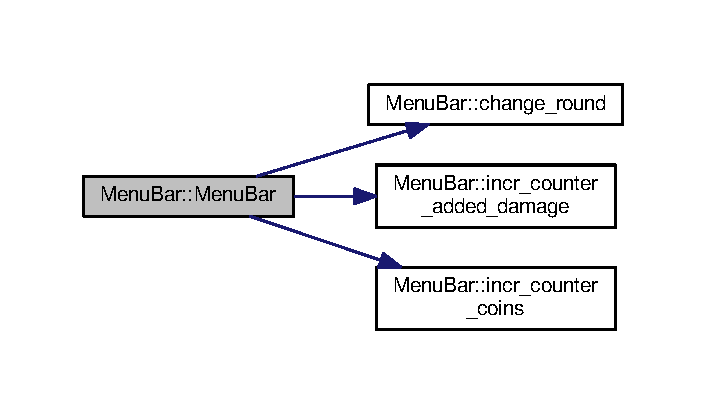
\includegraphics[width=339pt]{classMenuBar_a76a0ec8b0b4cba2775fa71e1791efc6d_cgraph}
\end{center}
\end{figure}




\subsection{Методы}
\index{Menu\+Bar@{Menu\+Bar}!change\+\_\+round@{change\+\_\+round}}
\index{change\+\_\+round@{change\+\_\+round}!Menu\+Bar@{Menu\+Bar}}
\subsubsection[{\texorpdfstring{change\+\_\+round()}{change_round()}}]{\setlength{\rightskip}{0pt plus 5cm}void Menu\+Bar\+::change\+\_\+round (
\begin{DoxyParamCaption}
{}
\end{DoxyParamCaption}
)\hspace{0.3cm}{\ttfamily [inline]}}\hypertarget{classMenuBar_a803dd882281e407e0494d2e5c45962bc}{}\label{classMenuBar_a803dd882281e407e0494d2e5c45962bc}


Граф вызова функции\+:\nopagebreak
\begin{figure}[H]
\begin{center}
\leavevmode
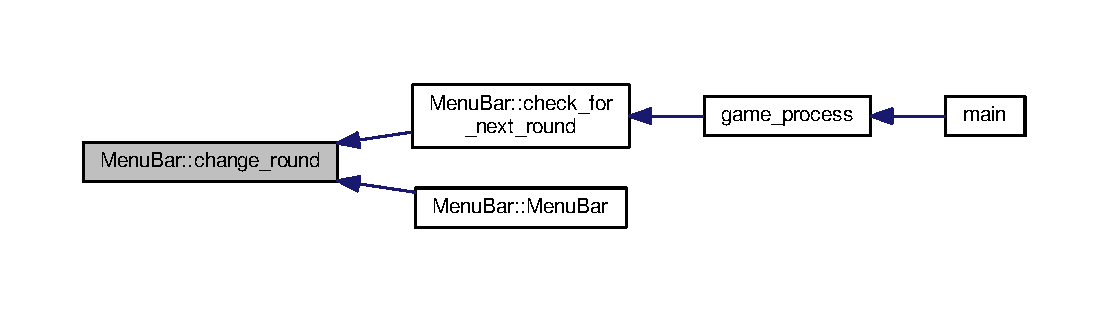
\includegraphics[width=350pt]{classMenuBar_a803dd882281e407e0494d2e5c45962bc_icgraph}
\end{center}
\end{figure}


\index{Menu\+Bar@{Menu\+Bar}!check\+\_\+for\+\_\+next\+\_\+round@{check\+\_\+for\+\_\+next\+\_\+round}}
\index{check\+\_\+for\+\_\+next\+\_\+round@{check\+\_\+for\+\_\+next\+\_\+round}!Menu\+Bar@{Menu\+Bar}}
\subsubsection[{\texorpdfstring{check\+\_\+for\+\_\+next\+\_\+round(sf\+::\+Clock \&clock, int add\+To\+Timer, int \&added\+Dmg\+In\+Perct, int \&added\+Hp\+In\+Perct)}{check_for_next_round(sf::Clock &clock, int addToTimer, int &addedDmgInPerct, int &addedHpInPerct)}}]{\setlength{\rightskip}{0pt plus 5cm}void Menu\+Bar\+::check\+\_\+for\+\_\+next\+\_\+round (
\begin{DoxyParamCaption}
\item[{sf\+::\+Clock \&}]{clock, }
\item[{int}]{add\+To\+Timer, }
\item[{int \&}]{added\+Dmg\+In\+Perct, }
\item[{int \&}]{added\+Hp\+In\+Perct}
\end{DoxyParamCaption}
)\hspace{0.3cm}{\ttfamily [inline]}}\hypertarget{classMenuBar_ab23d3bd560cb6a83deddad9ca2880c5b}{}\label{classMenuBar_ab23d3bd560cb6a83deddad9ca2880c5b}


Граф вызовов\+:\nopagebreak
\begin{figure}[H]
\begin{center}
\leavevmode
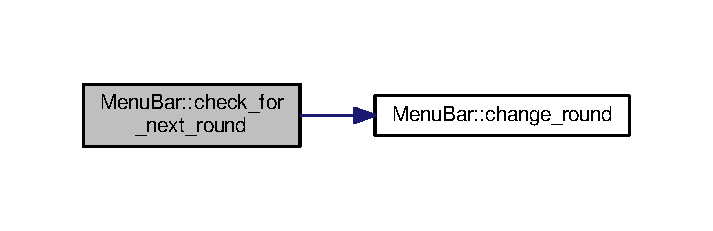
\includegraphics[width=342pt]{classMenuBar_ab23d3bd560cb6a83deddad9ca2880c5b_cgraph}
\end{center}
\end{figure}




Граф вызова функции\+:\nopagebreak
\begin{figure}[H]
\begin{center}
\leavevmode
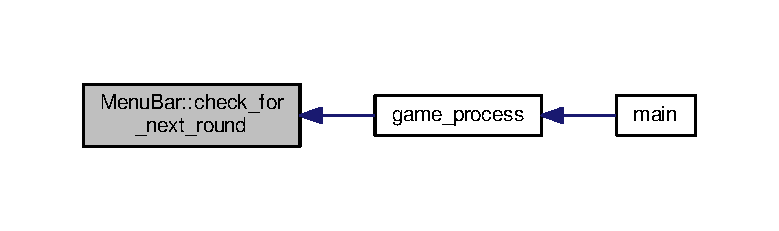
\includegraphics[width=350pt]{classMenuBar_ab23d3bd560cb6a83deddad9ca2880c5b_icgraph}
\end{center}
\end{figure}


\index{Menu\+Bar@{Menu\+Bar}!incr\+\_\+counter\+\_\+added\+\_\+damage@{incr\+\_\+counter\+\_\+added\+\_\+damage}}
\index{incr\+\_\+counter\+\_\+added\+\_\+damage@{incr\+\_\+counter\+\_\+added\+\_\+damage}!Menu\+Bar@{Menu\+Bar}}
\subsubsection[{\texorpdfstring{incr\+\_\+counter\+\_\+added\+\_\+damage(int value)}{incr_counter_added_damage(int value)}}]{\setlength{\rightskip}{0pt plus 5cm}void Menu\+Bar\+::incr\+\_\+counter\+\_\+added\+\_\+damage (
\begin{DoxyParamCaption}
\item[{int}]{value}
\end{DoxyParamCaption}
)\hspace{0.3cm}{\ttfamily [inline]}}\hypertarget{classMenuBar_a7a4dec33f791733c1babad22ac06d6e3}{}\label{classMenuBar_a7a4dec33f791733c1babad22ac06d6e3}


Граф вызова функции\+:\nopagebreak
\begin{figure}[H]
\begin{center}
\leavevmode
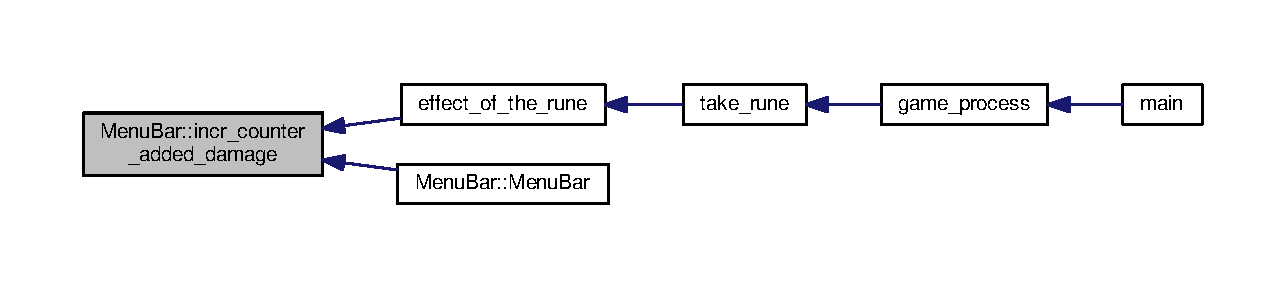
\includegraphics[width=350pt]{classMenuBar_a7a4dec33f791733c1babad22ac06d6e3_icgraph}
\end{center}
\end{figure}


\index{Menu\+Bar@{Menu\+Bar}!incr\+\_\+counter\+\_\+coins@{incr\+\_\+counter\+\_\+coins}}
\index{incr\+\_\+counter\+\_\+coins@{incr\+\_\+counter\+\_\+coins}!Menu\+Bar@{Menu\+Bar}}
\subsubsection[{\texorpdfstring{incr\+\_\+counter\+\_\+coins(int value)}{incr_counter_coins(int value)}}]{\setlength{\rightskip}{0pt plus 5cm}void Menu\+Bar\+::incr\+\_\+counter\+\_\+coins (
\begin{DoxyParamCaption}
\item[{int}]{value}
\end{DoxyParamCaption}
)\hspace{0.3cm}{\ttfamily [inline]}}\hypertarget{classMenuBar_a8517c956a4d36cdacdcb42989b5dccf3}{}\label{classMenuBar_a8517c956a4d36cdacdcb42989b5dccf3}


Граф вызова функции\+:\nopagebreak
\begin{figure}[H]
\begin{center}
\leavevmode
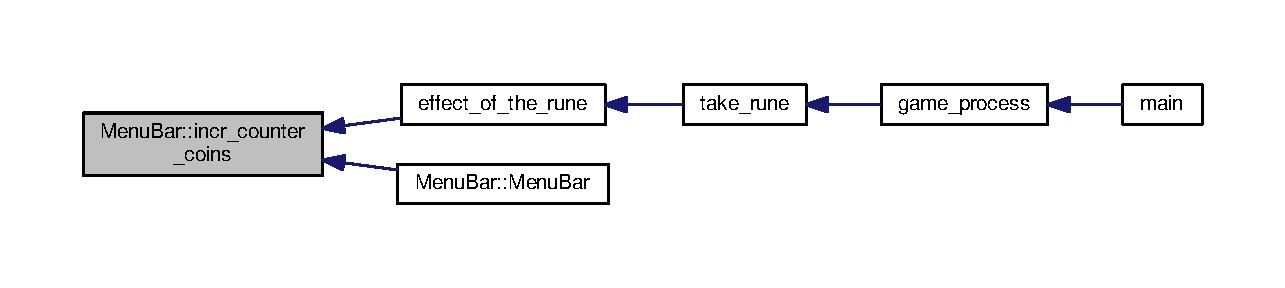
\includegraphics[width=350pt]{classMenuBar_a8517c956a4d36cdacdcb42989b5dccf3_icgraph}
\end{center}
\end{figure}




\subsection{Поля}
\index{Menu\+Bar@{Menu\+Bar}!basis\+\_\+damage@{basis\+\_\+damage}}
\index{basis\+\_\+damage@{basis\+\_\+damage}!Menu\+Bar@{Menu\+Bar}}
\subsubsection[{\texorpdfstring{basis\+\_\+damage}{basis_damage}}]{\setlength{\rightskip}{0pt plus 5cm}sf\+::\+Text Menu\+Bar\+::basis\+\_\+damage}\hypertarget{classMenuBar_a3093b55d6033fe43bf05afa0c6c9b1a8}{}\label{classMenuBar_a3093b55d6033fe43bf05afa0c6c9b1a8}
\index{Menu\+Bar@{Menu\+Bar}!Continue\+Text@{Continue\+Text}}
\index{Continue\+Text@{Continue\+Text}!Menu\+Bar@{Menu\+Bar}}
\subsubsection[{\texorpdfstring{Continue\+Text}{ContinueText}}]{\setlength{\rightskip}{0pt plus 5cm}sf\+::\+Text Menu\+Bar\+::\+Continue\+Text}\hypertarget{classMenuBar_aa01962756e77381b16471f863ed3c9c0}{}\label{classMenuBar_aa01962756e77381b16471f863ed3c9c0}
\index{Menu\+Bar@{Menu\+Bar}!counter\+Added\+Damage@{counter\+Added\+Damage}}
\index{counter\+Added\+Damage@{counter\+Added\+Damage}!Menu\+Bar@{Menu\+Bar}}
\subsubsection[{\texorpdfstring{counter\+Added\+Damage}{counterAddedDamage}}]{\setlength{\rightskip}{0pt plus 5cm}int Menu\+Bar\+::counter\+Added\+Damage}\hypertarget{classMenuBar_aca77c1b966ce3084c899dab8268cefc5}{}\label{classMenuBar_aca77c1b966ce3084c899dab8268cefc5}
\index{Menu\+Bar@{Menu\+Bar}!Exit\+Text@{Exit\+Text}}
\index{Exit\+Text@{Exit\+Text}!Menu\+Bar@{Menu\+Bar}}
\subsubsection[{\texorpdfstring{Exit\+Text}{ExitText}}]{\setlength{\rightskip}{0pt plus 5cm}sf\+::\+Text Menu\+Bar\+::\+Exit\+Text}\hypertarget{classMenuBar_ae9cd84f5d9a3b53d45b27cae6a7c44e6}{}\label{classMenuBar_ae9cd84f5d9a3b53d45b27cae6a7c44e6}
\index{Menu\+Bar@{Menu\+Bar}!h@{h}}
\index{h@{h}!Menu\+Bar@{Menu\+Bar}}
\subsubsection[{\texorpdfstring{h}{h}}]{\setlength{\rightskip}{0pt plus 5cm}int Menu\+Bar\+::h}\hypertarget{classMenuBar_a47f733e89c961de1ff15c2534b2c6f9b}{}\label{classMenuBar_a47f733e89c961de1ff15c2534b2c6f9b}
\index{Menu\+Bar@{Menu\+Bar}!icon\+Counter\+Added\+Damage@{icon\+Counter\+Added\+Damage}}
\index{icon\+Counter\+Added\+Damage@{icon\+Counter\+Added\+Damage}!Menu\+Bar@{Menu\+Bar}}
\subsubsection[{\texorpdfstring{icon\+Counter\+Added\+Damage}{iconCounterAddedDamage}}]{\setlength{\rightskip}{0pt plus 5cm}sf\+::\+Sprite Menu\+Bar\+::icon\+Counter\+Added\+Damage}\hypertarget{classMenuBar_a4bd5e603c2fc8611f804f69d82786077}{}\label{classMenuBar_a4bd5e603c2fc8611f804f69d82786077}
\index{Menu\+Bar@{Menu\+Bar}!icon\+Counter\+Coins@{icon\+Counter\+Coins}}
\index{icon\+Counter\+Coins@{icon\+Counter\+Coins}!Menu\+Bar@{Menu\+Bar}}
\subsubsection[{\texorpdfstring{icon\+Counter\+Coins}{iconCounterCoins}}]{\setlength{\rightskip}{0pt plus 5cm}sf\+::\+Sprite Menu\+Bar\+::icon\+Counter\+Coins}\hypertarget{classMenuBar_a05af15dc315210fef5dc78cd30a1e213}{}\label{classMenuBar_a05af15dc315210fef5dc78cd30a1e213}
\index{Menu\+Bar@{Menu\+Bar}!menubarline@{menubarline}}
\index{menubarline@{menubarline}!Menu\+Bar@{Menu\+Bar}}
\subsubsection[{\texorpdfstring{menubarline}{menubarline}}]{\setlength{\rightskip}{0pt plus 5cm}sf\+::\+Sprite Menu\+Bar\+::menubarline}\hypertarget{classMenuBar_a7c9348add51432373a0ac9ba34e0cc4a}{}\label{classMenuBar_a7c9348add51432373a0ac9ba34e0cc4a}
\index{Menu\+Bar@{Menu\+Bar}!pause\+Button@{pause\+Button}}
\index{pause\+Button@{pause\+Button}!Menu\+Bar@{Menu\+Bar}}
\subsubsection[{\texorpdfstring{pause\+Button}{pauseButton}}]{\setlength{\rightskip}{0pt plus 5cm}sf\+::\+Sprite Menu\+Bar\+::pause\+Button}\hypertarget{classMenuBar_a607b5c0461ef7951f3c0476bfd2ff00f}{}\label{classMenuBar_a607b5c0461ef7951f3c0476bfd2ff00f}
\index{Menu\+Bar@{Menu\+Bar}!pause\+Button\+Text@{pause\+Button\+Text}}
\index{pause\+Button\+Text@{pause\+Button\+Text}!Menu\+Bar@{Menu\+Bar}}
\subsubsection[{\texorpdfstring{pause\+Button\+Text}{pauseButtonText}}]{\setlength{\rightskip}{0pt plus 5cm}sf\+::\+Sprite Menu\+Bar\+::pause\+Button\+Text}\hypertarget{classMenuBar_a68d781e6301956723cf9826650ad7d2c}{}\label{classMenuBar_a68d781e6301956723cf9826650ad7d2c}
\index{Menu\+Bar@{Menu\+Bar}!Pause\+Menu@{Pause\+Menu}}
\index{Pause\+Menu@{Pause\+Menu}!Menu\+Bar@{Menu\+Bar}}
\subsubsection[{\texorpdfstring{Pause\+Menu}{PauseMenu}}]{\setlength{\rightskip}{0pt plus 5cm}sf\+::\+Sprite Menu\+Bar\+::\+Pause\+Menu}\hypertarget{classMenuBar_a8ba645ebcb1785788ea4763822fac236}{}\label{classMenuBar_a8ba645ebcb1785788ea4763822fac236}
\index{Menu\+Bar@{Menu\+Bar}!Pause\+Menu\+Button\+Continue@{Pause\+Menu\+Button\+Continue}}
\index{Pause\+Menu\+Button\+Continue@{Pause\+Menu\+Button\+Continue}!Menu\+Bar@{Menu\+Bar}}
\subsubsection[{\texorpdfstring{Pause\+Menu\+Button\+Continue}{PauseMenuButtonContinue}}]{\setlength{\rightskip}{0pt plus 5cm}sf\+::\+Sprite Menu\+Bar\+::\+Pause\+Menu\+Button\+Continue}\hypertarget{classMenuBar_a85b1a76501dd0d2ab5989a36b18299f2}{}\label{classMenuBar_a85b1a76501dd0d2ab5989a36b18299f2}
\index{Menu\+Bar@{Menu\+Bar}!Pause\+Menu\+Button\+Exit@{Pause\+Menu\+Button\+Exit}}
\index{Pause\+Menu\+Button\+Exit@{Pause\+Menu\+Button\+Exit}!Menu\+Bar@{Menu\+Bar}}
\subsubsection[{\texorpdfstring{Pause\+Menu\+Button\+Exit}{PauseMenuButtonExit}}]{\setlength{\rightskip}{0pt plus 5cm}sf\+::\+Sprite Menu\+Bar\+::\+Pause\+Menu\+Button\+Exit}\hypertarget{classMenuBar_a985fe3e19ae94063f676bcedab881b21}{}\label{classMenuBar_a985fe3e19ae94063f676bcedab881b21}
\index{Menu\+Bar@{Menu\+Bar}!round\+Text@{round\+Text}}
\index{round\+Text@{round\+Text}!Menu\+Bar@{Menu\+Bar}}
\subsubsection[{\texorpdfstring{round\+Text}{roundText}}]{\setlength{\rightskip}{0pt plus 5cm}sf\+::\+Text Menu\+Bar\+::round\+Text}\hypertarget{classMenuBar_af2f5d854bc3f91aec40595f84c232be3}{}\label{classMenuBar_af2f5d854bc3f91aec40595f84c232be3}
\index{Menu\+Bar@{Menu\+Bar}!text\+Counter\+Added\+Damage@{text\+Counter\+Added\+Damage}}
\index{text\+Counter\+Added\+Damage@{text\+Counter\+Added\+Damage}!Menu\+Bar@{Menu\+Bar}}
\subsubsection[{\texorpdfstring{text\+Counter\+Added\+Damage}{textCounterAddedDamage}}]{\setlength{\rightskip}{0pt plus 5cm}sf\+::\+Text Menu\+Bar\+::text\+Counter\+Added\+Damage}\hypertarget{classMenuBar_a91e93f244c42b092b1ac1708ad2376e0}{}\label{classMenuBar_a91e93f244c42b092b1ac1708ad2376e0}
\index{Menu\+Bar@{Menu\+Bar}!text\+Counter\+Coins@{text\+Counter\+Coins}}
\index{text\+Counter\+Coins@{text\+Counter\+Coins}!Menu\+Bar@{Menu\+Bar}}
\subsubsection[{\texorpdfstring{text\+Counter\+Coins}{textCounterCoins}}]{\setlength{\rightskip}{0pt plus 5cm}sf\+::\+Text Menu\+Bar\+::text\+Counter\+Coins}\hypertarget{classMenuBar_ade87fea2a3773189c1c984f78598354f}{}\label{classMenuBar_ade87fea2a3773189c1c984f78598354f}
\index{Menu\+Bar@{Menu\+Bar}!w@{w}}
\index{w@{w}!Menu\+Bar@{Menu\+Bar}}
\subsubsection[{\texorpdfstring{w}{w}}]{\setlength{\rightskip}{0pt plus 5cm}int Menu\+Bar\+::w}\hypertarget{classMenuBar_a3e9680e7db9109858b09c1ade97fd5d4}{}\label{classMenuBar_a3e9680e7db9109858b09c1ade97fd5d4}

\hypertarget{classGameObject_1_1Runes_1_1Plus__damage}{}\section{Класс Game\+Object\+:\+:Runes\+:\+:Plus\+\_\+damage}
\label{classGameObject_1_1Runes_1_1Plus__damage}\index{Game\+Object\+::\+Runes\+::\+Plus\+\_\+damage@{Game\+Object\+::\+Runes\+::\+Plus\+\_\+damage}}


The \hyperlink{classGameObject_1_1Runes_1_1Plus__damage}{Plus\+\_\+damage} class.  




{\ttfamily \#include $<$game\+\_\+objects.\+h$>$}

\subsection*{Открытые члены}
\begin{DoxyCompactItemize}
\item 
\hyperlink{classGameObject_1_1Runes_1_1Plus__damage_a9ed01c21040fda145bc262ca6c2d9822}{Plus\+\_\+damage} ()
\end{DoxyCompactItemize}
\subsection*{Поля данных}
\begin{DoxyCompactItemize}
\item 
sf\+::\+Sprite \hyperlink{classGameObject_1_1Runes_1_1Plus__damage_a1286be03fc1312928d408528f8bddf25}{sprite}
\item 
float \hyperlink{classGameObject_1_1Runes_1_1Plus__damage_a67e0a90ac6bd68ecca36ef410c87a505}{w}
\item 
float \hyperlink{classGameObject_1_1Runes_1_1Plus__damage_acb2903ce736dae31e937abbf7cb132b4}{h}
\item 
float \hyperlink{classGameObject_1_1Runes_1_1Plus__damage_a09b7ecb5d9db3dad1942c5c3d08299f5}{frames}
\item 
float \hyperlink{classGameObject_1_1Runes_1_1Plus__damage_a1993229d8a137d5dc6feb4b572a98bc0}{current\+\_\+frame}
\item 
int \hyperlink{classGameObject_1_1Runes_1_1Plus__damage_a8d6f33861ad270c2f0c01abea24fd432}{added\+Damage}
\end{DoxyCompactItemize}


\subsection{Подробное описание}
The \hyperlink{classGameObject_1_1Runes_1_1Plus__damage}{Plus\+\_\+damage} class. 

\subsection{Конструктор(ы)}
\index{Game\+Object\+::\+Runes\+::\+Plus\+\_\+damage@{Game\+Object\+::\+Runes\+::\+Plus\+\_\+damage}!Plus\+\_\+damage@{Plus\+\_\+damage}}
\index{Plus\+\_\+damage@{Plus\+\_\+damage}!Game\+Object\+::\+Runes\+::\+Plus\+\_\+damage@{Game\+Object\+::\+Runes\+::\+Plus\+\_\+damage}}
\subsubsection[{\texorpdfstring{Plus\+\_\+damage()}{Plus_damage()}}]{\setlength{\rightskip}{0pt plus 5cm}Game\+Object\+::\+Runes\+::\+Plus\+\_\+damage\+::\+Plus\+\_\+damage (
\begin{DoxyParamCaption}
{}
\end{DoxyParamCaption}
)\hspace{0.3cm}{\ttfamily [inline]}}\hypertarget{classGameObject_1_1Runes_1_1Plus__damage_a9ed01c21040fda145bc262ca6c2d9822}{}\label{classGameObject_1_1Runes_1_1Plus__damage_a9ed01c21040fda145bc262ca6c2d9822}


\subsection{Поля}
\index{Game\+Object\+::\+Runes\+::\+Plus\+\_\+damage@{Game\+Object\+::\+Runes\+::\+Plus\+\_\+damage}!added\+Damage@{added\+Damage}}
\index{added\+Damage@{added\+Damage}!Game\+Object\+::\+Runes\+::\+Plus\+\_\+damage@{Game\+Object\+::\+Runes\+::\+Plus\+\_\+damage}}
\subsubsection[{\texorpdfstring{added\+Damage}{addedDamage}}]{\setlength{\rightskip}{0pt plus 5cm}int Game\+Object\+::\+Runes\+::\+Plus\+\_\+damage\+::added\+Damage}\hypertarget{classGameObject_1_1Runes_1_1Plus__damage_a8d6f33861ad270c2f0c01abea24fd432}{}\label{classGameObject_1_1Runes_1_1Plus__damage_a8d6f33861ad270c2f0c01abea24fd432}
\index{Game\+Object\+::\+Runes\+::\+Plus\+\_\+damage@{Game\+Object\+::\+Runes\+::\+Plus\+\_\+damage}!current\+\_\+frame@{current\+\_\+frame}}
\index{current\+\_\+frame@{current\+\_\+frame}!Game\+Object\+::\+Runes\+::\+Plus\+\_\+damage@{Game\+Object\+::\+Runes\+::\+Plus\+\_\+damage}}
\subsubsection[{\texorpdfstring{current\+\_\+frame}{current_frame}}]{\setlength{\rightskip}{0pt plus 5cm}float Game\+Object\+::\+Runes\+::\+Plus\+\_\+damage\+::current\+\_\+frame}\hypertarget{classGameObject_1_1Runes_1_1Plus__damage_a1993229d8a137d5dc6feb4b572a98bc0}{}\label{classGameObject_1_1Runes_1_1Plus__damage_a1993229d8a137d5dc6feb4b572a98bc0}
\index{Game\+Object\+::\+Runes\+::\+Plus\+\_\+damage@{Game\+Object\+::\+Runes\+::\+Plus\+\_\+damage}!frames@{frames}}
\index{frames@{frames}!Game\+Object\+::\+Runes\+::\+Plus\+\_\+damage@{Game\+Object\+::\+Runes\+::\+Plus\+\_\+damage}}
\subsubsection[{\texorpdfstring{frames}{frames}}]{\setlength{\rightskip}{0pt plus 5cm}float Game\+Object\+::\+Runes\+::\+Plus\+\_\+damage\+::frames}\hypertarget{classGameObject_1_1Runes_1_1Plus__damage_a09b7ecb5d9db3dad1942c5c3d08299f5}{}\label{classGameObject_1_1Runes_1_1Plus__damage_a09b7ecb5d9db3dad1942c5c3d08299f5}
\index{Game\+Object\+::\+Runes\+::\+Plus\+\_\+damage@{Game\+Object\+::\+Runes\+::\+Plus\+\_\+damage}!h@{h}}
\index{h@{h}!Game\+Object\+::\+Runes\+::\+Plus\+\_\+damage@{Game\+Object\+::\+Runes\+::\+Plus\+\_\+damage}}
\subsubsection[{\texorpdfstring{h}{h}}]{\setlength{\rightskip}{0pt plus 5cm}float Game\+Object\+::\+Runes\+::\+Plus\+\_\+damage\+::h}\hypertarget{classGameObject_1_1Runes_1_1Plus__damage_acb2903ce736dae31e937abbf7cb132b4}{}\label{classGameObject_1_1Runes_1_1Plus__damage_acb2903ce736dae31e937abbf7cb132b4}
\index{Game\+Object\+::\+Runes\+::\+Plus\+\_\+damage@{Game\+Object\+::\+Runes\+::\+Plus\+\_\+damage}!sprite@{sprite}}
\index{sprite@{sprite}!Game\+Object\+::\+Runes\+::\+Plus\+\_\+damage@{Game\+Object\+::\+Runes\+::\+Plus\+\_\+damage}}
\subsubsection[{\texorpdfstring{sprite}{sprite}}]{\setlength{\rightskip}{0pt plus 5cm}sf\+::\+Sprite Game\+Object\+::\+Runes\+::\+Plus\+\_\+damage\+::sprite}\hypertarget{classGameObject_1_1Runes_1_1Plus__damage_a1286be03fc1312928d408528f8bddf25}{}\label{classGameObject_1_1Runes_1_1Plus__damage_a1286be03fc1312928d408528f8bddf25}
\index{Game\+Object\+::\+Runes\+::\+Plus\+\_\+damage@{Game\+Object\+::\+Runes\+::\+Plus\+\_\+damage}!w@{w}}
\index{w@{w}!Game\+Object\+::\+Runes\+::\+Plus\+\_\+damage@{Game\+Object\+::\+Runes\+::\+Plus\+\_\+damage}}
\subsubsection[{\texorpdfstring{w}{w}}]{\setlength{\rightskip}{0pt plus 5cm}float Game\+Object\+::\+Runes\+::\+Plus\+\_\+damage\+::w}\hypertarget{classGameObject_1_1Runes_1_1Plus__damage_a67e0a90ac6bd68ecca36ef410c87a505}{}\label{classGameObject_1_1Runes_1_1Plus__damage_a67e0a90ac6bd68ecca36ef410c87a505}

\hypertarget{classGameObject_1_1Runes}{}\section{Класс Game\+Object\+:\+:Runes}
\label{classGameObject_1_1Runes}\index{Game\+Object\+::\+Runes@{Game\+Object\+::\+Runes}}


The \hyperlink{classGameObject_1_1Runes}{Runes} class.  




{\ttfamily \#include $<$game\+\_\+objects.\+h$>$}



Граф связей класса Game\+Object\+:\+:Runes\+:\nopagebreak
\begin{figure}[H]
\begin{center}
\leavevmode
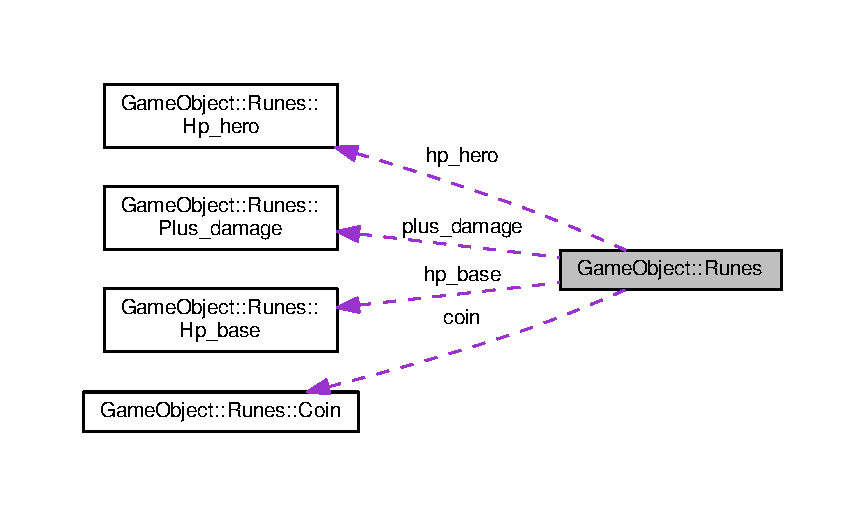
\includegraphics[width=350pt]{classGameObject_1_1Runes__coll__graph}
\end{center}
\end{figure}
\subsection*{Структуры данных}
\begin{DoxyCompactItemize}
\item 
class \hyperlink{classGameObject_1_1Runes_1_1Coin}{Coin}
\begin{DoxyCompactList}\small\item\em The \hyperlink{classGameObject_1_1Runes_1_1Coin}{Coin} class. \end{DoxyCompactList}\item 
class \hyperlink{classGameObject_1_1Runes_1_1Hp__base}{Hp\+\_\+base}
\begin{DoxyCompactList}\small\item\em The \hyperlink{classGameObject_1_1Runes_1_1Hp__base}{Hp\+\_\+base} class. \end{DoxyCompactList}\item 
class \hyperlink{classGameObject_1_1Runes_1_1Hp__hero}{Hp\+\_\+hero}
\begin{DoxyCompactList}\small\item\em The \hyperlink{classGameObject_1_1Runes_1_1Hp__hero}{Hp\+\_\+hero} class. \end{DoxyCompactList}\item 
class \hyperlink{classGameObject_1_1Runes_1_1Plus__damage}{Plus\+\_\+damage}
\begin{DoxyCompactList}\small\item\em The \hyperlink{classGameObject_1_1Runes_1_1Plus__damage}{Plus\+\_\+damage} class. \end{DoxyCompactList}\end{DoxyCompactItemize}
\subsection*{Открытые члены}
\begin{DoxyCompactItemize}
\item 
void \hyperlink{classGameObject_1_1Runes_a67bc85b74264e40b12f59b0c54e9c0db}{update\+\_\+frame} (int \&type)
\end{DoxyCompactItemize}
\subsection*{Поля данных}
\begin{DoxyCompactItemize}
\item 
\hyperlink{classGameObject_1_1Runes_1_1Hp__hero}{Hp\+\_\+hero} \hyperlink{classGameObject_1_1Runes_aa5a714bdf8756bf51223127bfe153ad7}{hp\+\_\+hero}
\item 
\hyperlink{classGameObject_1_1Runes_1_1Hp__base}{Hp\+\_\+base} \hyperlink{classGameObject_1_1Runes_a70b4206ddc0146c08a105c95291b26e9}{hp\+\_\+base}
\item 
\hyperlink{classGameObject_1_1Runes_1_1Plus__damage}{Plus\+\_\+damage} \hyperlink{classGameObject_1_1Runes_ab8155a9e9c17e969e26cb2cf05d8d7aa}{plus\+\_\+damage}
\item 
\hyperlink{classGameObject_1_1Runes_1_1Coin}{Coin} \hyperlink{classGameObject_1_1Runes_ae9001d326154583d3a43efb165d00296}{coin}
\end{DoxyCompactItemize}


\subsection{Подробное описание}
The \hyperlink{classGameObject_1_1Runes}{Runes} class. 

\begin{DoxySeeAlso}{См. также}
\hyperlink{classGameObject_1_1Runes_1_1Hp__hero}{Hp\+\_\+hero}, \hyperlink{classGameObject_1_1Runes_1_1Hp__base}{Hp\+\_\+base}, \hyperlink{classGameObject_1_1Runes_1_1Plus__damage}{Plus\+\_\+damage}, \hyperlink{classGameObject_1_1Runes_1_1Coin}{Coin} 
\end{DoxySeeAlso}


\subsection{Методы}
\index{Game\+Object\+::\+Runes@{Game\+Object\+::\+Runes}!update\+\_\+frame@{update\+\_\+frame}}
\index{update\+\_\+frame@{update\+\_\+frame}!Game\+Object\+::\+Runes@{Game\+Object\+::\+Runes}}
\subsubsection[{\texorpdfstring{update\+\_\+frame(int \&type)}{update_frame(int &type)}}]{\setlength{\rightskip}{0pt plus 5cm}void Game\+Object\+::\+Runes\+::update\+\_\+frame (
\begin{DoxyParamCaption}
\item[{int \&}]{type}
\end{DoxyParamCaption}
)\hspace{0.3cm}{\ttfamily [inline]}}\hypertarget{classGameObject_1_1Runes_a67bc85b74264e40b12f59b0c54e9c0db}{}\label{classGameObject_1_1Runes_a67bc85b74264e40b12f59b0c54e9c0db}


\subsection{Поля}
\index{Game\+Object\+::\+Runes@{Game\+Object\+::\+Runes}!coin@{coin}}
\index{coin@{coin}!Game\+Object\+::\+Runes@{Game\+Object\+::\+Runes}}
\subsubsection[{\texorpdfstring{coin}{coin}}]{\setlength{\rightskip}{0pt plus 5cm}{\bf Coin} Game\+Object\+::\+Runes\+::coin}\hypertarget{classGameObject_1_1Runes_ae9001d326154583d3a43efb165d00296}{}\label{classGameObject_1_1Runes_ae9001d326154583d3a43efb165d00296}
\index{Game\+Object\+::\+Runes@{Game\+Object\+::\+Runes}!hp\+\_\+base@{hp\+\_\+base}}
\index{hp\+\_\+base@{hp\+\_\+base}!Game\+Object\+::\+Runes@{Game\+Object\+::\+Runes}}
\subsubsection[{\texorpdfstring{hp\+\_\+base}{hp_base}}]{\setlength{\rightskip}{0pt plus 5cm}{\bf Hp\+\_\+base} Game\+Object\+::\+Runes\+::hp\+\_\+base}\hypertarget{classGameObject_1_1Runes_a70b4206ddc0146c08a105c95291b26e9}{}\label{classGameObject_1_1Runes_a70b4206ddc0146c08a105c95291b26e9}
\index{Game\+Object\+::\+Runes@{Game\+Object\+::\+Runes}!hp\+\_\+hero@{hp\+\_\+hero}}
\index{hp\+\_\+hero@{hp\+\_\+hero}!Game\+Object\+::\+Runes@{Game\+Object\+::\+Runes}}
\subsubsection[{\texorpdfstring{hp\+\_\+hero}{hp_hero}}]{\setlength{\rightskip}{0pt plus 5cm}{\bf Hp\+\_\+hero} Game\+Object\+::\+Runes\+::hp\+\_\+hero}\hypertarget{classGameObject_1_1Runes_aa5a714bdf8756bf51223127bfe153ad7}{}\label{classGameObject_1_1Runes_aa5a714bdf8756bf51223127bfe153ad7}
\index{Game\+Object\+::\+Runes@{Game\+Object\+::\+Runes}!plus\+\_\+damage@{plus\+\_\+damage}}
\index{plus\+\_\+damage@{plus\+\_\+damage}!Game\+Object\+::\+Runes@{Game\+Object\+::\+Runes}}
\subsubsection[{\texorpdfstring{plus\+\_\+damage}{plus_damage}}]{\setlength{\rightskip}{0pt plus 5cm}{\bf Plus\+\_\+damage} Game\+Object\+::\+Runes\+::plus\+\_\+damage}\hypertarget{classGameObject_1_1Runes_ab8155a9e9c17e969e26cb2cf05d8d7aa}{}\label{classGameObject_1_1Runes_ab8155a9e9c17e969e26cb2cf05d8d7aa}

\hypertarget{classToolBar}{}\section{Класс Tool\+Bar}
\label{classToolBar}\index{Tool\+Bar@{Tool\+Bar}}


Праметры счётчиков,выводимых в нижней полоске игровогоокна  




{\ttfamily \#include $<$tool\+\_\+bar.\+h$>$}

\subsection*{Открытые члены}
\begin{DoxyCompactItemize}
\item 
void \hyperlink{classToolBar_acb6ec6dffc23783cd110667e3a012c2a}{get\+\_\+time} (sf\+::\+Clock \&clock, std\+::minstd\+\_\+rand \&simple\+\_\+rand)
\item 
void \hyperlink{classToolBar_a704da8346e935b2724aba9d80bbdd66b}{randomize\+Rune} (std\+::minstd\+\_\+rand \&simple\+\_\+rand)
\item 
void \hyperlink{classToolBar_ae8d52640262d6e25d07e65ad5cfe8a54}{add\+\_\+to\+\_\+time} (sf\+::\+Clock \&clock)
\item 
void \hyperlink{classToolBar_a6c030d2393dd9ad33fb51e59b9ae9d6b}{reset\+\_\+clock} (sf\+::\+Clock \&clock)
\item 
bool \hyperlink{classToolBar_a7f2fbad05b0511c585283fe5377c6096}{change\+\_\+hero\+\_\+base\+\_\+hp} (std\+::string object, std\+::string str, int value, int \&objecthealth)
\item 
void \hyperlink{classToolBar_a4cc86d8767581aaa437f851d5782c61e}{change\+\_\+enemy\+\_\+hp\+\_\+line} (int health, int Max\+Health, int enemy\+Type)
\item 
void \hyperlink{classToolBar_a6b8c6075b58347e259cabf177adfd687}{update\+\_\+spawn\+Timer} ()
\item 
\hyperlink{classToolBar_a998467428b7984217db78653412f2c68}{Tool\+Bar} ()
\end{DoxyCompactItemize}
\subsection*{Поля данных}
\begin{DoxyCompactItemize}
\item 
sf\+::\+Sprite \hyperlink{classToolBar_a32ef55bee6542ce2f9856b1252a5bc00}{toolbarline}
\item 
sf\+::\+Text \hyperlink{classToolBar_a5e34d6e961f9f8d200f11d5c90d10121}{timer}
\item 
sf\+::\+Sprite \hyperlink{classToolBar_a282b572766a7fb833266997f6776aa76}{icon\+Clock}
\item 
int \hyperlink{classToolBar_aa4978a990d85761cb5ab6d60ab5b081c}{add\+To\+Timer}
\item 
sf\+::\+Sprite \hyperlink{classToolBar_a188e889517db774fa50f3babdcc61054}{hp\+\_\+hero\+\_\+red}
\item 
sf\+::\+Sprite \hyperlink{classToolBar_a65b3cfcbb54e656f98639620717bc701}{hp\+\_\+hero\+\_\+green}
\item 
sf\+::\+Text \hyperlink{classToolBar_abb14f5c369cee727893e9eae44594e26}{text\+H\+HP}
\item 
sf\+::\+Sprite \hyperlink{classToolBar_a3a23db17ec632acd38594ba68d5d0584}{icon\+H\+Phero}
\item 
sf\+::\+Text \hyperlink{classToolBar_a30d2ccc2f04f7143b8df59947578b97d}{value\+H\+H\+Pof}
\item 
sf\+::\+Sprite \hyperlink{classToolBar_afb75ac14df5e61b9c50c93beda809415}{hp\+\_\+base\+\_\+red\+\_\+orange}
\item 
sf\+::\+Sprite \hyperlink{classToolBar_a72b41dd993c27b3cb5de4e8d3e7b1c54}{hp\+\_\+base\+\_\+green}
\item 
sf\+::\+Text \hyperlink{classToolBar_a471626dfedf4ed4efda3773701d55364}{text\+B\+HP}
\item 
sf\+::\+Sprite \hyperlink{classToolBar_a29febf7bc604146e8d0df1b041dc13c8}{icon\+H\+Pbase}
\item 
sf\+::\+Text \hyperlink{classToolBar_ae97f03f2157daabe56dd60b56b698e15}{value\+B\+H\+Pof}
\item 
sf\+::\+Sprite \hyperlink{classToolBar_adf6487dd1c7f42354e93702f45eefba6}{hp\+\_\+enemy\+\_\+red}
\item 
sf\+::\+Sprite \hyperlink{classToolBar_a63b820836b22bac6096fc2d947dc0227}{hp\+\_\+enemy\+\_\+green}
\item 
sf\+::\+Text \hyperlink{classToolBar_a9510aea21130fa29c71233c9acc0fcae}{text\+E\+HP}
\item 
sf\+::\+Sprite \hyperlink{classToolBar_a66d3f57460533b9a96c46a21144bc275}{icon\+H\+Penemy}
\item 
sf\+::\+Sprite \hyperlink{classToolBar_ab5eb6994e23b6cf2013ed4914ee3f36e}{icon\+Enemy}
\item 
sf\+::\+Text \hyperlink{classToolBar_ad3512dba4d37c5c08645b3ded0331f98}{value\+E\+H\+Pof}
\item 
sf\+::\+Sprite \hyperlink{classToolBar_a2c12e5622569daf38c009fa2906a045c}{icon\+Dead\+Enemy}
\item 
bool \hyperlink{classToolBar_a833dab17c0f9a6a82fa6e97b59e6c2e7}{draw\+Icon\+Dead\+Enemy}
\item 
sf\+::\+Sprite \hyperlink{classToolBar_afc2823f5c1dd0927a04867d034f80f62}{icon\+Timer}
\item 
sf\+::\+Text \hyperlink{classToolBar_a255b295736a1540e3f21a1436c2925c8}{spawn\+Timer}
\item 
int \hyperlink{classToolBar_a6254f8067b6a4487cbb1eedaf8fc5db7}{seconds\+Until\+Spawn}
\item 
int \hyperlink{classToolBar_a02a8dc52a45537dabcd5b2322271a745}{buffer\+Seconds}
\item 
int \hyperlink{classToolBar_adb3e79f3152cda0389c9077e716859f0}{type\+Randomed\+Rune}
\item 
bool \hyperlink{classToolBar_a759e611d4eb9396a75b8825236eeff6c}{randomize\+Coordinates}
\end{DoxyCompactItemize}


\subsection{Подробное описание}
Праметры счётчиков,выводимых в нижней полоске игровогоокна 

\subsection{Конструктор(ы)}
\index{Tool\+Bar@{Tool\+Bar}!Tool\+Bar@{Tool\+Bar}}
\index{Tool\+Bar@{Tool\+Bar}!Tool\+Bar@{Tool\+Bar}}
\subsubsection[{\texorpdfstring{Tool\+Bar()}{ToolBar()}}]{\setlength{\rightskip}{0pt plus 5cm}Tool\+Bar\+::\+Tool\+Bar (
\begin{DoxyParamCaption}
{}
\end{DoxyParamCaption}
)\hspace{0.3cm}{\ttfamily [inline]}}\hypertarget{classToolBar_a998467428b7984217db78653412f2c68}{}\label{classToolBar_a998467428b7984217db78653412f2c68}


Граф вызовов\+:\nopagebreak
\begin{figure}[H]
\begin{center}
\leavevmode
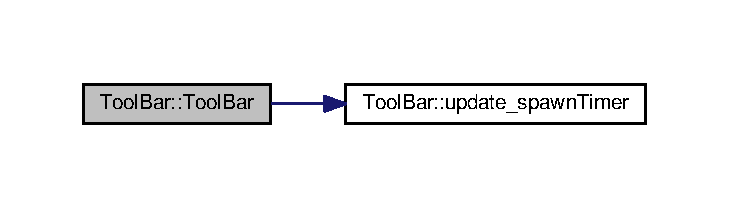
\includegraphics[width=350pt]{classToolBar_a998467428b7984217db78653412f2c68_cgraph}
\end{center}
\end{figure}




\subsection{Методы}
\index{Tool\+Bar@{Tool\+Bar}!add\+\_\+to\+\_\+time@{add\+\_\+to\+\_\+time}}
\index{add\+\_\+to\+\_\+time@{add\+\_\+to\+\_\+time}!Tool\+Bar@{Tool\+Bar}}
\subsubsection[{\texorpdfstring{add\+\_\+to\+\_\+time(sf\+::\+Clock \&clock)}{add_to_time(sf::Clock &clock)}}]{\setlength{\rightskip}{0pt plus 5cm}void Tool\+Bar\+::add\+\_\+to\+\_\+time (
\begin{DoxyParamCaption}
\item[{sf\+::\+Clock \&}]{clock}
\end{DoxyParamCaption}
)\hspace{0.3cm}{\ttfamily [inline]}}\hypertarget{classToolBar_ae8d52640262d6e25d07e65ad5cfe8a54}{}\label{classToolBar_ae8d52640262d6e25d07e65ad5cfe8a54}


Граф вызова функции\+:\nopagebreak
\begin{figure}[H]
\begin{center}
\leavevmode
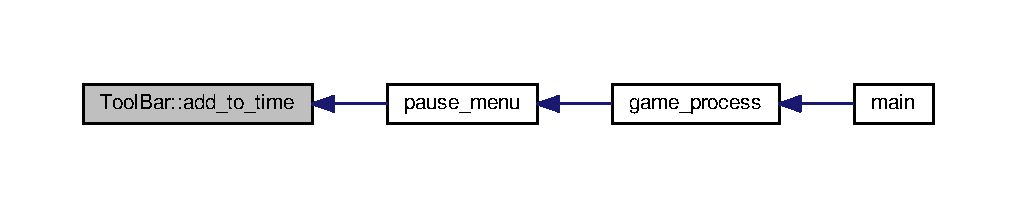
\includegraphics[width=350pt]{classToolBar_ae8d52640262d6e25d07e65ad5cfe8a54_icgraph}
\end{center}
\end{figure}


\index{Tool\+Bar@{Tool\+Bar}!change\+\_\+enemy\+\_\+hp\+\_\+line@{change\+\_\+enemy\+\_\+hp\+\_\+line}}
\index{change\+\_\+enemy\+\_\+hp\+\_\+line@{change\+\_\+enemy\+\_\+hp\+\_\+line}!Tool\+Bar@{Tool\+Bar}}
\subsubsection[{\texorpdfstring{change\+\_\+enemy\+\_\+hp\+\_\+line(int health, int Max\+Health, int enemy\+Type)}{change_enemy_hp_line(int health, int MaxHealth, int enemyType)}}]{\setlength{\rightskip}{0pt plus 5cm}void Tool\+Bar\+::change\+\_\+enemy\+\_\+hp\+\_\+line (
\begin{DoxyParamCaption}
\item[{int}]{health, }
\item[{int}]{Max\+Health, }
\item[{int}]{enemy\+Type}
\end{DoxyParamCaption}
)\hspace{0.3cm}{\ttfamily [inline]}}\hypertarget{classToolBar_a4cc86d8767581aaa437f851d5782c61e}{}\label{classToolBar_a4cc86d8767581aaa437f851d5782c61e}


Граф вызова функции\+:\nopagebreak
\begin{figure}[H]
\begin{center}
\leavevmode
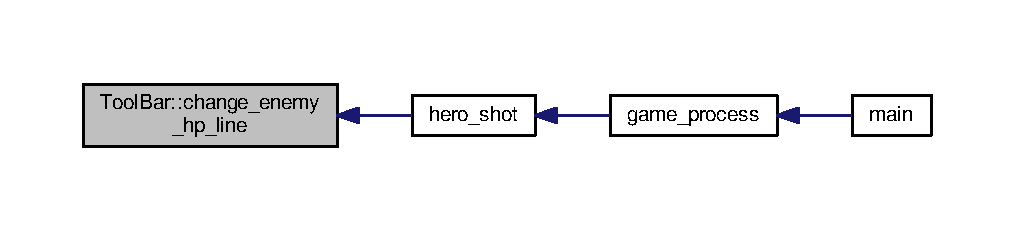
\includegraphics[width=350pt]{classToolBar_a4cc86d8767581aaa437f851d5782c61e_icgraph}
\end{center}
\end{figure}


\index{Tool\+Bar@{Tool\+Bar}!change\+\_\+hero\+\_\+base\+\_\+hp@{change\+\_\+hero\+\_\+base\+\_\+hp}}
\index{change\+\_\+hero\+\_\+base\+\_\+hp@{change\+\_\+hero\+\_\+base\+\_\+hp}!Tool\+Bar@{Tool\+Bar}}
\subsubsection[{\texorpdfstring{change\+\_\+hero\+\_\+base\+\_\+hp(std\+::string object, std\+::string str, int value, int \&objecthealth)}{change_hero_base_hp(std::string object, std::string str, int value, int &objecthealth)}}]{\setlength{\rightskip}{0pt plus 5cm}bool Tool\+Bar\+::change\+\_\+hero\+\_\+base\+\_\+hp (
\begin{DoxyParamCaption}
\item[{std\+::string}]{object, }
\item[{std\+::string}]{str, }
\item[{int}]{value, }
\item[{int \&}]{objecthealth}
\end{DoxyParamCaption}
)\hspace{0.3cm}{\ttfamily [inline]}}\hypertarget{classToolBar_a7f2fbad05b0511c585283fe5377c6096}{}\label{classToolBar_a7f2fbad05b0511c585283fe5377c6096}


Граф вызова функции\+:\nopagebreak
\begin{figure}[H]
\begin{center}
\leavevmode
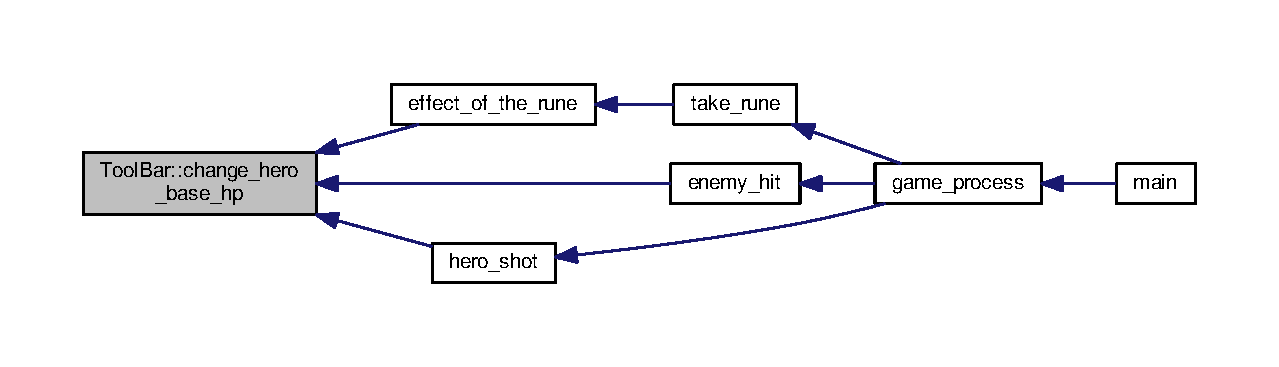
\includegraphics[width=350pt]{classToolBar_a7f2fbad05b0511c585283fe5377c6096_icgraph}
\end{center}
\end{figure}


\index{Tool\+Bar@{Tool\+Bar}!get\+\_\+time@{get\+\_\+time}}
\index{get\+\_\+time@{get\+\_\+time}!Tool\+Bar@{Tool\+Bar}}
\subsubsection[{\texorpdfstring{get\+\_\+time(sf\+::\+Clock \&clock, std\+::minstd\+\_\+rand \&simple\+\_\+rand)}{get_time(sf::Clock &clock, std::minstd_rand &simple_rand)}}]{\setlength{\rightskip}{0pt plus 5cm}void Tool\+Bar\+::get\+\_\+time (
\begin{DoxyParamCaption}
\item[{sf\+::\+Clock \&}]{clock, }
\item[{std\+::minstd\+\_\+rand \&}]{simple\+\_\+rand}
\end{DoxyParamCaption}
)\hspace{0.3cm}{\ttfamily [inline]}}\hypertarget{classToolBar_acb6ec6dffc23783cd110667e3a012c2a}{}\label{classToolBar_acb6ec6dffc23783cd110667e3a012c2a}


Граф вызовов\+:\nopagebreak
\begin{figure}[H]
\begin{center}
\leavevmode
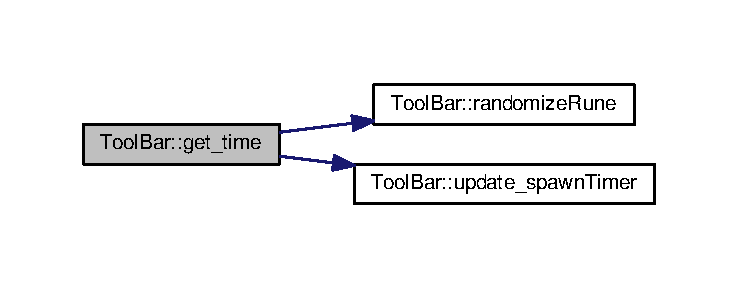
\includegraphics[width=350pt]{classToolBar_acb6ec6dffc23783cd110667e3a012c2a_cgraph}
\end{center}
\end{figure}




Граф вызова функции\+:\nopagebreak
\begin{figure}[H]
\begin{center}
\leavevmode
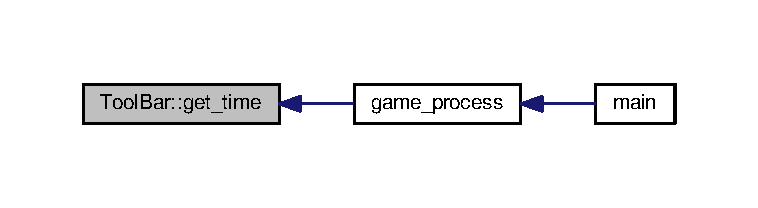
\includegraphics[width=350pt]{classToolBar_acb6ec6dffc23783cd110667e3a012c2a_icgraph}
\end{center}
\end{figure}


\index{Tool\+Bar@{Tool\+Bar}!randomize\+Rune@{randomize\+Rune}}
\index{randomize\+Rune@{randomize\+Rune}!Tool\+Bar@{Tool\+Bar}}
\subsubsection[{\texorpdfstring{randomize\+Rune(std\+::minstd\+\_\+rand \&simple\+\_\+rand)}{randomizeRune(std::minstd_rand &simple_rand)}}]{\setlength{\rightskip}{0pt plus 5cm}void Tool\+Bar\+::randomize\+Rune (
\begin{DoxyParamCaption}
\item[{std\+::minstd\+\_\+rand \&}]{simple\+\_\+rand}
\end{DoxyParamCaption}
)\hspace{0.3cm}{\ttfamily [inline]}}\hypertarget{classToolBar_a704da8346e935b2724aba9d80bbdd66b}{}\label{classToolBar_a704da8346e935b2724aba9d80bbdd66b}


Граф вызова функции\+:\nopagebreak
\begin{figure}[H]
\begin{center}
\leavevmode
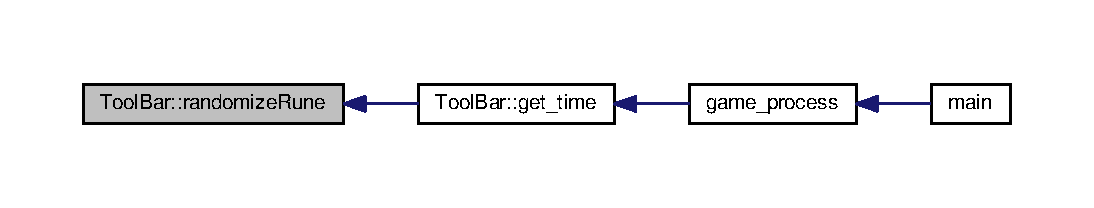
\includegraphics[width=350pt]{classToolBar_a704da8346e935b2724aba9d80bbdd66b_icgraph}
\end{center}
\end{figure}


\index{Tool\+Bar@{Tool\+Bar}!reset\+\_\+clock@{reset\+\_\+clock}}
\index{reset\+\_\+clock@{reset\+\_\+clock}!Tool\+Bar@{Tool\+Bar}}
\subsubsection[{\texorpdfstring{reset\+\_\+clock(sf\+::\+Clock \&clock)}{reset_clock(sf::Clock &clock)}}]{\setlength{\rightskip}{0pt plus 5cm}void Tool\+Bar\+::reset\+\_\+clock (
\begin{DoxyParamCaption}
\item[{sf\+::\+Clock \&}]{clock}
\end{DoxyParamCaption}
)\hspace{0.3cm}{\ttfamily [inline]}}\hypertarget{classToolBar_a6c030d2393dd9ad33fb51e59b9ae9d6b}{}\label{classToolBar_a6c030d2393dd9ad33fb51e59b9ae9d6b}


Граф вызова функции\+:\nopagebreak
\begin{figure}[H]
\begin{center}
\leavevmode
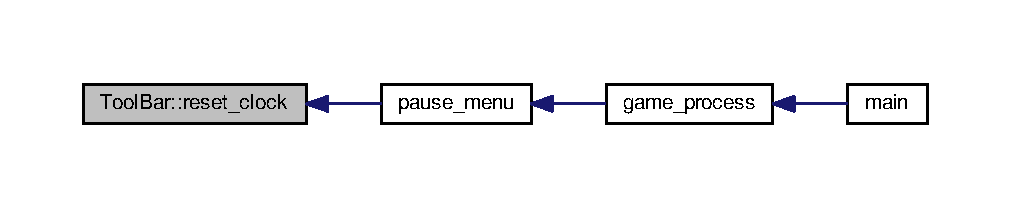
\includegraphics[width=350pt]{classToolBar_a6c030d2393dd9ad33fb51e59b9ae9d6b_icgraph}
\end{center}
\end{figure}


\index{Tool\+Bar@{Tool\+Bar}!update\+\_\+spawn\+Timer@{update\+\_\+spawn\+Timer}}
\index{update\+\_\+spawn\+Timer@{update\+\_\+spawn\+Timer}!Tool\+Bar@{Tool\+Bar}}
\subsubsection[{\texorpdfstring{update\+\_\+spawn\+Timer()}{update_spawnTimer()}}]{\setlength{\rightskip}{0pt plus 5cm}void Tool\+Bar\+::update\+\_\+spawn\+Timer (
\begin{DoxyParamCaption}
{}
\end{DoxyParamCaption}
)\hspace{0.3cm}{\ttfamily [inline]}}\hypertarget{classToolBar_a6b8c6075b58347e259cabf177adfd687}{}\label{classToolBar_a6b8c6075b58347e259cabf177adfd687}


Граф вызова функции\+:\nopagebreak
\begin{figure}[H]
\begin{center}
\leavevmode
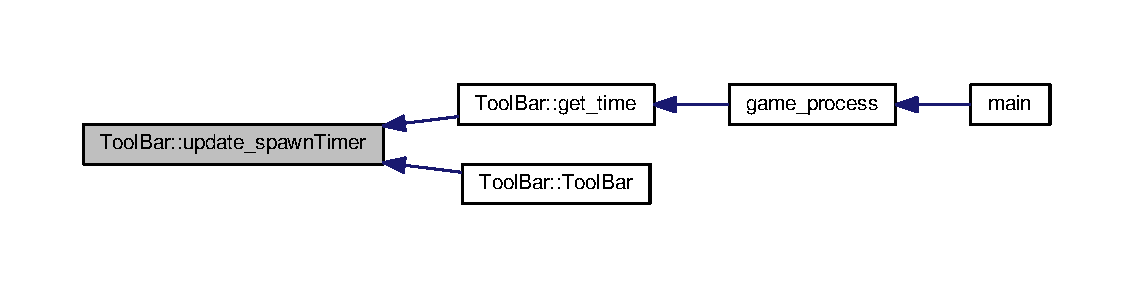
\includegraphics[width=350pt]{classToolBar_a6b8c6075b58347e259cabf177adfd687_icgraph}
\end{center}
\end{figure}




\subsection{Поля}
\index{Tool\+Bar@{Tool\+Bar}!add\+To\+Timer@{add\+To\+Timer}}
\index{add\+To\+Timer@{add\+To\+Timer}!Tool\+Bar@{Tool\+Bar}}
\subsubsection[{\texorpdfstring{add\+To\+Timer}{addToTimer}}]{\setlength{\rightskip}{0pt plus 5cm}int Tool\+Bar\+::add\+To\+Timer}\hypertarget{classToolBar_aa4978a990d85761cb5ab6d60ab5b081c}{}\label{classToolBar_aa4978a990d85761cb5ab6d60ab5b081c}
\index{Tool\+Bar@{Tool\+Bar}!buffer\+Seconds@{buffer\+Seconds}}
\index{buffer\+Seconds@{buffer\+Seconds}!Tool\+Bar@{Tool\+Bar}}
\subsubsection[{\texorpdfstring{buffer\+Seconds}{bufferSeconds}}]{\setlength{\rightskip}{0pt plus 5cm}int Tool\+Bar\+::buffer\+Seconds}\hypertarget{classToolBar_a02a8dc52a45537dabcd5b2322271a745}{}\label{classToolBar_a02a8dc52a45537dabcd5b2322271a745}
\index{Tool\+Bar@{Tool\+Bar}!draw\+Icon\+Dead\+Enemy@{draw\+Icon\+Dead\+Enemy}}
\index{draw\+Icon\+Dead\+Enemy@{draw\+Icon\+Dead\+Enemy}!Tool\+Bar@{Tool\+Bar}}
\subsubsection[{\texorpdfstring{draw\+Icon\+Dead\+Enemy}{drawIconDeadEnemy}}]{\setlength{\rightskip}{0pt plus 5cm}bool Tool\+Bar\+::draw\+Icon\+Dead\+Enemy}\hypertarget{classToolBar_a833dab17c0f9a6a82fa6e97b59e6c2e7}{}\label{classToolBar_a833dab17c0f9a6a82fa6e97b59e6c2e7}
\index{Tool\+Bar@{Tool\+Bar}!hp\+\_\+base\+\_\+green@{hp\+\_\+base\+\_\+green}}
\index{hp\+\_\+base\+\_\+green@{hp\+\_\+base\+\_\+green}!Tool\+Bar@{Tool\+Bar}}
\subsubsection[{\texorpdfstring{hp\+\_\+base\+\_\+green}{hp_base_green}}]{\setlength{\rightskip}{0pt plus 5cm}sf\+::\+Sprite Tool\+Bar\+::hp\+\_\+base\+\_\+green}\hypertarget{classToolBar_a72b41dd993c27b3cb5de4e8d3e7b1c54}{}\label{classToolBar_a72b41dd993c27b3cb5de4e8d3e7b1c54}
\index{Tool\+Bar@{Tool\+Bar}!hp\+\_\+base\+\_\+red\+\_\+orange@{hp\+\_\+base\+\_\+red\+\_\+orange}}
\index{hp\+\_\+base\+\_\+red\+\_\+orange@{hp\+\_\+base\+\_\+red\+\_\+orange}!Tool\+Bar@{Tool\+Bar}}
\subsubsection[{\texorpdfstring{hp\+\_\+base\+\_\+red\+\_\+orange}{hp_base_red_orange}}]{\setlength{\rightskip}{0pt plus 5cm}sf\+::\+Sprite Tool\+Bar\+::hp\+\_\+base\+\_\+red\+\_\+orange}\hypertarget{classToolBar_afb75ac14df5e61b9c50c93beda809415}{}\label{classToolBar_afb75ac14df5e61b9c50c93beda809415}
\index{Tool\+Bar@{Tool\+Bar}!hp\+\_\+enemy\+\_\+green@{hp\+\_\+enemy\+\_\+green}}
\index{hp\+\_\+enemy\+\_\+green@{hp\+\_\+enemy\+\_\+green}!Tool\+Bar@{Tool\+Bar}}
\subsubsection[{\texorpdfstring{hp\+\_\+enemy\+\_\+green}{hp_enemy_green}}]{\setlength{\rightskip}{0pt plus 5cm}sf\+::\+Sprite Tool\+Bar\+::hp\+\_\+enemy\+\_\+green}\hypertarget{classToolBar_a63b820836b22bac6096fc2d947dc0227}{}\label{classToolBar_a63b820836b22bac6096fc2d947dc0227}
\index{Tool\+Bar@{Tool\+Bar}!hp\+\_\+enemy\+\_\+red@{hp\+\_\+enemy\+\_\+red}}
\index{hp\+\_\+enemy\+\_\+red@{hp\+\_\+enemy\+\_\+red}!Tool\+Bar@{Tool\+Bar}}
\subsubsection[{\texorpdfstring{hp\+\_\+enemy\+\_\+red}{hp_enemy_red}}]{\setlength{\rightskip}{0pt plus 5cm}sf\+::\+Sprite Tool\+Bar\+::hp\+\_\+enemy\+\_\+red}\hypertarget{classToolBar_adf6487dd1c7f42354e93702f45eefba6}{}\label{classToolBar_adf6487dd1c7f42354e93702f45eefba6}
\index{Tool\+Bar@{Tool\+Bar}!hp\+\_\+hero\+\_\+green@{hp\+\_\+hero\+\_\+green}}
\index{hp\+\_\+hero\+\_\+green@{hp\+\_\+hero\+\_\+green}!Tool\+Bar@{Tool\+Bar}}
\subsubsection[{\texorpdfstring{hp\+\_\+hero\+\_\+green}{hp_hero_green}}]{\setlength{\rightskip}{0pt plus 5cm}sf\+::\+Sprite Tool\+Bar\+::hp\+\_\+hero\+\_\+green}\hypertarget{classToolBar_a65b3cfcbb54e656f98639620717bc701}{}\label{classToolBar_a65b3cfcbb54e656f98639620717bc701}
\index{Tool\+Bar@{Tool\+Bar}!hp\+\_\+hero\+\_\+red@{hp\+\_\+hero\+\_\+red}}
\index{hp\+\_\+hero\+\_\+red@{hp\+\_\+hero\+\_\+red}!Tool\+Bar@{Tool\+Bar}}
\subsubsection[{\texorpdfstring{hp\+\_\+hero\+\_\+red}{hp_hero_red}}]{\setlength{\rightskip}{0pt plus 5cm}sf\+::\+Sprite Tool\+Bar\+::hp\+\_\+hero\+\_\+red}\hypertarget{classToolBar_a188e889517db774fa50f3babdcc61054}{}\label{classToolBar_a188e889517db774fa50f3babdcc61054}
\index{Tool\+Bar@{Tool\+Bar}!icon\+Clock@{icon\+Clock}}
\index{icon\+Clock@{icon\+Clock}!Tool\+Bar@{Tool\+Bar}}
\subsubsection[{\texorpdfstring{icon\+Clock}{iconClock}}]{\setlength{\rightskip}{0pt plus 5cm}sf\+::\+Sprite Tool\+Bar\+::icon\+Clock}\hypertarget{classToolBar_a282b572766a7fb833266997f6776aa76}{}\label{classToolBar_a282b572766a7fb833266997f6776aa76}
\index{Tool\+Bar@{Tool\+Bar}!icon\+Dead\+Enemy@{icon\+Dead\+Enemy}}
\index{icon\+Dead\+Enemy@{icon\+Dead\+Enemy}!Tool\+Bar@{Tool\+Bar}}
\subsubsection[{\texorpdfstring{icon\+Dead\+Enemy}{iconDeadEnemy}}]{\setlength{\rightskip}{0pt plus 5cm}sf\+::\+Sprite Tool\+Bar\+::icon\+Dead\+Enemy}\hypertarget{classToolBar_a2c12e5622569daf38c009fa2906a045c}{}\label{classToolBar_a2c12e5622569daf38c009fa2906a045c}
\index{Tool\+Bar@{Tool\+Bar}!icon\+Enemy@{icon\+Enemy}}
\index{icon\+Enemy@{icon\+Enemy}!Tool\+Bar@{Tool\+Bar}}
\subsubsection[{\texorpdfstring{icon\+Enemy}{iconEnemy}}]{\setlength{\rightskip}{0pt plus 5cm}sf\+::\+Sprite Tool\+Bar\+::icon\+Enemy}\hypertarget{classToolBar_ab5eb6994e23b6cf2013ed4914ee3f36e}{}\label{classToolBar_ab5eb6994e23b6cf2013ed4914ee3f36e}
\index{Tool\+Bar@{Tool\+Bar}!icon\+H\+Pbase@{icon\+H\+Pbase}}
\index{icon\+H\+Pbase@{icon\+H\+Pbase}!Tool\+Bar@{Tool\+Bar}}
\subsubsection[{\texorpdfstring{icon\+H\+Pbase}{iconHPbase}}]{\setlength{\rightskip}{0pt plus 5cm}sf\+::\+Sprite Tool\+Bar\+::icon\+H\+Pbase}\hypertarget{classToolBar_a29febf7bc604146e8d0df1b041dc13c8}{}\label{classToolBar_a29febf7bc604146e8d0df1b041dc13c8}
\index{Tool\+Bar@{Tool\+Bar}!icon\+H\+Penemy@{icon\+H\+Penemy}}
\index{icon\+H\+Penemy@{icon\+H\+Penemy}!Tool\+Bar@{Tool\+Bar}}
\subsubsection[{\texorpdfstring{icon\+H\+Penemy}{iconHPenemy}}]{\setlength{\rightskip}{0pt plus 5cm}sf\+::\+Sprite Tool\+Bar\+::icon\+H\+Penemy}\hypertarget{classToolBar_a66d3f57460533b9a96c46a21144bc275}{}\label{classToolBar_a66d3f57460533b9a96c46a21144bc275}
\index{Tool\+Bar@{Tool\+Bar}!icon\+H\+Phero@{icon\+H\+Phero}}
\index{icon\+H\+Phero@{icon\+H\+Phero}!Tool\+Bar@{Tool\+Bar}}
\subsubsection[{\texorpdfstring{icon\+H\+Phero}{iconHPhero}}]{\setlength{\rightskip}{0pt plus 5cm}sf\+::\+Sprite Tool\+Bar\+::icon\+H\+Phero}\hypertarget{classToolBar_a3a23db17ec632acd38594ba68d5d0584}{}\label{classToolBar_a3a23db17ec632acd38594ba68d5d0584}
\index{Tool\+Bar@{Tool\+Bar}!icon\+Timer@{icon\+Timer}}
\index{icon\+Timer@{icon\+Timer}!Tool\+Bar@{Tool\+Bar}}
\subsubsection[{\texorpdfstring{icon\+Timer}{iconTimer}}]{\setlength{\rightskip}{0pt plus 5cm}sf\+::\+Sprite Tool\+Bar\+::icon\+Timer}\hypertarget{classToolBar_afc2823f5c1dd0927a04867d034f80f62}{}\label{classToolBar_afc2823f5c1dd0927a04867d034f80f62}
\index{Tool\+Bar@{Tool\+Bar}!randomize\+Coordinates@{randomize\+Coordinates}}
\index{randomize\+Coordinates@{randomize\+Coordinates}!Tool\+Bar@{Tool\+Bar}}
\subsubsection[{\texorpdfstring{randomize\+Coordinates}{randomizeCoordinates}}]{\setlength{\rightskip}{0pt plus 5cm}bool Tool\+Bar\+::randomize\+Coordinates}\hypertarget{classToolBar_a759e611d4eb9396a75b8825236eeff6c}{}\label{classToolBar_a759e611d4eb9396a75b8825236eeff6c}
\index{Tool\+Bar@{Tool\+Bar}!seconds\+Until\+Spawn@{seconds\+Until\+Spawn}}
\index{seconds\+Until\+Spawn@{seconds\+Until\+Spawn}!Tool\+Bar@{Tool\+Bar}}
\subsubsection[{\texorpdfstring{seconds\+Until\+Spawn}{secondsUntilSpawn}}]{\setlength{\rightskip}{0pt plus 5cm}int Tool\+Bar\+::seconds\+Until\+Spawn}\hypertarget{classToolBar_a6254f8067b6a4487cbb1eedaf8fc5db7}{}\label{classToolBar_a6254f8067b6a4487cbb1eedaf8fc5db7}
\index{Tool\+Bar@{Tool\+Bar}!spawn\+Timer@{spawn\+Timer}}
\index{spawn\+Timer@{spawn\+Timer}!Tool\+Bar@{Tool\+Bar}}
\subsubsection[{\texorpdfstring{spawn\+Timer}{spawnTimer}}]{\setlength{\rightskip}{0pt plus 5cm}sf\+::\+Text Tool\+Bar\+::spawn\+Timer}\hypertarget{classToolBar_a255b295736a1540e3f21a1436c2925c8}{}\label{classToolBar_a255b295736a1540e3f21a1436c2925c8}
\index{Tool\+Bar@{Tool\+Bar}!text\+B\+HP@{text\+B\+HP}}
\index{text\+B\+HP@{text\+B\+HP}!Tool\+Bar@{Tool\+Bar}}
\subsubsection[{\texorpdfstring{text\+B\+HP}{textBHP}}]{\setlength{\rightskip}{0pt plus 5cm}sf\+::\+Text Tool\+Bar\+::text\+B\+HP}\hypertarget{classToolBar_a471626dfedf4ed4efda3773701d55364}{}\label{classToolBar_a471626dfedf4ed4efda3773701d55364}
\index{Tool\+Bar@{Tool\+Bar}!text\+E\+HP@{text\+E\+HP}}
\index{text\+E\+HP@{text\+E\+HP}!Tool\+Bar@{Tool\+Bar}}
\subsubsection[{\texorpdfstring{text\+E\+HP}{textEHP}}]{\setlength{\rightskip}{0pt plus 5cm}sf\+::\+Text Tool\+Bar\+::text\+E\+HP}\hypertarget{classToolBar_a9510aea21130fa29c71233c9acc0fcae}{}\label{classToolBar_a9510aea21130fa29c71233c9acc0fcae}
\index{Tool\+Bar@{Tool\+Bar}!text\+H\+HP@{text\+H\+HP}}
\index{text\+H\+HP@{text\+H\+HP}!Tool\+Bar@{Tool\+Bar}}
\subsubsection[{\texorpdfstring{text\+H\+HP}{textHHP}}]{\setlength{\rightskip}{0pt plus 5cm}sf\+::\+Text Tool\+Bar\+::text\+H\+HP}\hypertarget{classToolBar_abb14f5c369cee727893e9eae44594e26}{}\label{classToolBar_abb14f5c369cee727893e9eae44594e26}
\index{Tool\+Bar@{Tool\+Bar}!timer@{timer}}
\index{timer@{timer}!Tool\+Bar@{Tool\+Bar}}
\subsubsection[{\texorpdfstring{timer}{timer}}]{\setlength{\rightskip}{0pt plus 5cm}sf\+::\+Text Tool\+Bar\+::timer}\hypertarget{classToolBar_a5e34d6e961f9f8d200f11d5c90d10121}{}\label{classToolBar_a5e34d6e961f9f8d200f11d5c90d10121}
\index{Tool\+Bar@{Tool\+Bar}!toolbarline@{toolbarline}}
\index{toolbarline@{toolbarline}!Tool\+Bar@{Tool\+Bar}}
\subsubsection[{\texorpdfstring{toolbarline}{toolbarline}}]{\setlength{\rightskip}{0pt plus 5cm}sf\+::\+Sprite Tool\+Bar\+::toolbarline}\hypertarget{classToolBar_a32ef55bee6542ce2f9856b1252a5bc00}{}\label{classToolBar_a32ef55bee6542ce2f9856b1252a5bc00}
\index{Tool\+Bar@{Tool\+Bar}!type\+Randomed\+Rune@{type\+Randomed\+Rune}}
\index{type\+Randomed\+Rune@{type\+Randomed\+Rune}!Tool\+Bar@{Tool\+Bar}}
\subsubsection[{\texorpdfstring{type\+Randomed\+Rune}{typeRandomedRune}}]{\setlength{\rightskip}{0pt plus 5cm}int Tool\+Bar\+::type\+Randomed\+Rune}\hypertarget{classToolBar_adb3e79f3152cda0389c9077e716859f0}{}\label{classToolBar_adb3e79f3152cda0389c9077e716859f0}
\index{Tool\+Bar@{Tool\+Bar}!value\+B\+H\+Pof@{value\+B\+H\+Pof}}
\index{value\+B\+H\+Pof@{value\+B\+H\+Pof}!Tool\+Bar@{Tool\+Bar}}
\subsubsection[{\texorpdfstring{value\+B\+H\+Pof}{valueBHPof}}]{\setlength{\rightskip}{0pt plus 5cm}sf\+::\+Text Tool\+Bar\+::value\+B\+H\+Pof}\hypertarget{classToolBar_ae97f03f2157daabe56dd60b56b698e15}{}\label{classToolBar_ae97f03f2157daabe56dd60b56b698e15}
\index{Tool\+Bar@{Tool\+Bar}!value\+E\+H\+Pof@{value\+E\+H\+Pof}}
\index{value\+E\+H\+Pof@{value\+E\+H\+Pof}!Tool\+Bar@{Tool\+Bar}}
\subsubsection[{\texorpdfstring{value\+E\+H\+Pof}{valueEHPof}}]{\setlength{\rightskip}{0pt plus 5cm}sf\+::\+Text Tool\+Bar\+::value\+E\+H\+Pof}\hypertarget{classToolBar_ad3512dba4d37c5c08645b3ded0331f98}{}\label{classToolBar_ad3512dba4d37c5c08645b3ded0331f98}
\index{Tool\+Bar@{Tool\+Bar}!value\+H\+H\+Pof@{value\+H\+H\+Pof}}
\index{value\+H\+H\+Pof@{value\+H\+H\+Pof}!Tool\+Bar@{Tool\+Bar}}
\subsubsection[{\texorpdfstring{value\+H\+H\+Pof}{valueHHPof}}]{\setlength{\rightskip}{0pt plus 5cm}sf\+::\+Text Tool\+Bar\+::value\+H\+H\+Pof}\hypertarget{classToolBar_a30d2ccc2f04f7143b8df59947578b97d}{}\label{classToolBar_a30d2ccc2f04f7143b8df59947578b97d}

\chapter{Файлы}
\hypertarget{base__hero__explosion_8cpp}{}\section{Файл /home/dzigen/inf1/\+C\+S/task12/\+Tower\+\_\+\+Defense\+\_\+\+Game/app/base\+\_\+hero\+\_\+explosion.cpp}
\label{base__hero__explosion_8cpp}\index{/home/dzigen/inf1/\+C\+S/task12/\+Tower\+\_\+\+Defense\+\_\+\+Game/app/base\+\_\+hero\+\_\+explosion.\+cpp@{/home/dzigen/inf1/\+C\+S/task12/\+Tower\+\_\+\+Defense\+\_\+\+Game/app/base\+\_\+hero\+\_\+explosion.\+cpp}}
{\ttfamily \#include \char`\"{}game\+\_\+objects.\+h\char`\"{}}\\*
{\ttfamily \#include \char`\"{}pause\+\_\+end\+\_\+menu.\+h\char`\"{}}\\*
Граф включаемых заголовочных файлов для base\+\_\+hero\+\_\+explosion.\+cpp\+:\nopagebreak
\begin{figure}[H]
\begin{center}
\leavevmode
\includegraphics[width=350pt]{base__hero__explosion_8cpp__incl}
\end{center}
\end{figure}
\subsection*{Функции}
\begin{DoxyCompactItemize}
\item 
void \hyperlink{group__heroBaseHandler_ga4b8f8d1c761e24c0a8480a7489d349d1}{base\+\_\+hero\+\_\+explosion} (sf\+::\+Render\+Window \&window, \hyperlink{classMenuBar}{Menu\+Bar} \&upper\+Parametr, \hyperlink{classToolBar}{Tool\+Bar} \&lower\+Parametr, \hyperlink{classCursors}{Cursors} \&cursor, \hyperlink{classGameObject}{Game\+Object} \&object, sf\+::\+Clock \&game\+Time)
\begin{DoxyCompactList}\small\item\em Отрисовка и анимация взрыва базы \end{DoxyCompactList}\end{DoxyCompactItemize}

\hypertarget{cursors_8h}{}\section{Файл /home/dzigen/inf1/\+C\+S/task12/\+Tower\+\_\+\+Defense\+\_\+\+Game/app/cursors.h}
\label{cursors_8h}\index{/home/dzigen/inf1/\+C\+S/task12/\+Tower\+\_\+\+Defense\+\_\+\+Game/app/cursors.\+h@{/home/dzigen/inf1/\+C\+S/task12/\+Tower\+\_\+\+Defense\+\_\+\+Game/app/cursors.\+h}}
{\ttfamily \#include $<$S\+F\+M\+L/\+Graphics.\+hpp$>$}\\*
Граф включаемых заголовочных файлов для cursors.\+h\+:\nopagebreak
\begin{figure}[H]
\begin{center}
\leavevmode
\includegraphics[width=201pt]{cursors_8h__incl}
\end{center}
\end{figure}
Граф файлов, в которые включается этот файл\+:\nopagebreak
\begin{figure}[H]
\begin{center}
\leavevmode
\includegraphics[width=350pt]{cursors_8h__dep__incl}
\end{center}
\end{figure}
\subsection*{Структуры данных}
\begin{DoxyCompactItemize}
\item 
class \hyperlink{classCursors}{Cursors}
\begin{DoxyCompactList}\small\item\em Хранимые параметры кастомного курсора в игре \end{DoxyCompactList}\end{DoxyCompactItemize}

\hypertarget{effect__of__the__rune_8cpp}{}\section{Файл /home/dzigen/inf1/\+C\+S/task12/\+Tower\+\_\+\+Defense\+\_\+\+Game/app/effect\+\_\+of\+\_\+the\+\_\+rune.cpp}
\label{effect__of__the__rune_8cpp}\index{/home/dzigen/inf1/\+C\+S/task12/\+Tower\+\_\+\+Defense\+\_\+\+Game/app/effect\+\_\+of\+\_\+the\+\_\+rune.\+cpp@{/home/dzigen/inf1/\+C\+S/task12/\+Tower\+\_\+\+Defense\+\_\+\+Game/app/effect\+\_\+of\+\_\+the\+\_\+rune.\+cpp}}
{\ttfamily \#include \char`\"{}game\+\_\+objects.\+h\char`\"{}}\\*
{\ttfamily \#include \char`\"{}tool\+\_\+bar.\+h\char`\"{}}\\*
{\ttfamily \#include \char`\"{}menu\+\_\+bar.\+h\char`\"{}}\\*
Граф включаемых заголовочных файлов для effect\+\_\+of\+\_\+the\+\_\+rune.\+cpp\+:\nopagebreak
\begin{figure}[H]
\begin{center}
\leavevmode
\includegraphics[width=350pt]{effect__of__the__rune_8cpp__incl}
\end{center}
\end{figure}
\subsection*{Функции}
\begin{DoxyCompactItemize}
\item 
void \hyperlink{group__runeHandler_ga0078b36ac662e224e1913996193c1c98}{effect\+\_\+of\+\_\+the\+\_\+rune} (\hyperlink{classGameObject}{Game\+Object} \&object, \hyperlink{classToolBar}{Tool\+Bar} \&toolbar, \hyperlink{classMenuBar}{Menu\+Bar} \&menubar)
\begin{DoxyCompactList}\small\item\em Обрабатывается эффект применения руны в соответствии с её типом \end{DoxyCompactList}\end{DoxyCompactItemize}

\hypertarget{end__game_8cpp}{}\section{Файл /home/dzigen/inf1/\+C\+S/task12/\+Tower\+\_\+\+Defense\+\_\+\+Game/app/end\+\_\+game.cpp}
\label{end__game_8cpp}\index{/home/dzigen/inf1/\+C\+S/task12/\+Tower\+\_\+\+Defense\+\_\+\+Game/app/end\+\_\+game.\+cpp@{/home/dzigen/inf1/\+C\+S/task12/\+Tower\+\_\+\+Defense\+\_\+\+Game/app/end\+\_\+game.\+cpp}}
{\ttfamily \#include $<$S\+F\+M\+L/\+Graphics.\+hpp$>$}\\*
{\ttfamily \#include \char`\"{}game\+\_\+objects.\+h\char`\"{}}\\*
{\ttfamily \#include \char`\"{}game\+\_\+end\+\_\+window.\+h\char`\"{}}\\*
Граф включаемых заголовочных файлов для end\+\_\+game.\+cpp\+:\nopagebreak
\begin{figure}[H]
\begin{center}
\leavevmode
\includegraphics[width=350pt]{end__game_8cpp__incl}
\end{center}
\end{figure}
\subsection*{Функции}
\begin{DoxyCompactItemize}
\item 
bool \hyperlink{group__menu_ga3259e0d309cf137b40488db0226f91f6}{end\+\_\+game} (\hyperlink{classGameObject}{Game\+Object} \&object, \hyperlink{classGameEndWindow}{Game\+End\+Window} \&end\+Window)
\begin{DoxyCompactList}\small\item\em Обработка завершения игрового цроцесса \end{DoxyCompactList}\end{DoxyCompactItemize}

\hypertarget{enemy__hit_8cpp}{}\section{Файл /home/dzigen/inf1/\+C\+S/task12/\+Tower\+\_\+\+Defense\+\_\+\+Game/app/enemy\+\_\+hit.cpp}
\label{enemy__hit_8cpp}\index{/home/dzigen/inf1/\+C\+S/task12/\+Tower\+\_\+\+Defense\+\_\+\+Game/app/enemy\+\_\+hit.\+cpp@{/home/dzigen/inf1/\+C\+S/task12/\+Tower\+\_\+\+Defense\+\_\+\+Game/app/enemy\+\_\+hit.\+cpp}}
{\ttfamily \#include $<$S\+F\+M\+L/\+Graphics.\+hpp$>$}\\*
{\ttfamily \#include \char`\"{}game\+\_\+objects.\+h\char`\"{}}\\*
{\ttfamily \#include \char`\"{}menu\+\_\+bar.\+h\char`\"{}}\\*
{\ttfamily \#include \char`\"{}tool\+\_\+bar.\+h\char`\"{}}\\*
{\ttfamily \#include $<$vector$>$}\\*
Граф включаемых заголовочных файлов для enemy\+\_\+hit.\+cpp\+:\nopagebreak
\begin{figure}[H]
\begin{center}
\leavevmode
\includegraphics[width=350pt]{enemy__hit_8cpp__incl}
\end{center}
\end{figure}
\subsection*{Функции}
\begin{DoxyCompactItemize}
\item 
void \hyperlink{group__enemyHandler_ga6965d0b7bc93883e1089dd9a326a584a}{enemy\+\_\+hit} (\hyperlink{classGameObject}{Game\+Object} \&object, \hyperlink{classToolBar}{Tool\+Bar} \&toolbar, float time)
\begin{DoxyCompactList}\small\item\em Обработка атаки врагов на карте игрового процесса \end{DoxyCompactList}\end{DoxyCompactItemize}

\hypertarget{game__draw_8cpp}{}\section{Файл /home/dzigen/inf1/\+C\+S/task12/\+Tower\+\_\+\+Defense\+\_\+\+Game/app/game\+\_\+draw.cpp}
\label{game__draw_8cpp}\index{/home/dzigen/inf1/\+C\+S/task12/\+Tower\+\_\+\+Defense\+\_\+\+Game/app/game\+\_\+draw.\+cpp@{/home/dzigen/inf1/\+C\+S/task12/\+Tower\+\_\+\+Defense\+\_\+\+Game/app/game\+\_\+draw.\+cpp}}
{\ttfamily \#include \char`\"{}cursors.\+h\char`\"{}}\\*
{\ttfamily \#include \char`\"{}menu\+\_\+bar.\+h\char`\"{}}\\*
{\ttfamily \#include \char`\"{}tool\+\_\+bar.\+h\char`\"{}}\\*
{\ttfamily \#include \char`\"{}game\+\_\+objects.\+h\char`\"{}}\\*
Граф включаемых заголовочных файлов для game\+\_\+draw.\+cpp\+:\nopagebreak
\begin{figure}[H]
\begin{center}
\leavevmode
\includegraphics[width=350pt]{game__draw_8cpp__incl}
\end{center}
\end{figure}
\subsection*{Функции}
\begin{DoxyCompactItemize}
\item 
void \hyperlink{group__mainLoop_gaf2266f0127d085329a1b7e092832e8a3}{game\+\_\+draw} (sf\+::\+Render\+Window \&window, \hyperlink{classMenuBar}{Menu\+Bar} \&upper\+Parametr, \hyperlink{classToolBar}{Tool\+Bar} \&lower\+Parametr, \hyperlink{classGameObject}{Game\+Object} \&object)
\begin{DoxyCompactList}\small\item\em Вывод игрового процесса в игровом окне \end{DoxyCompactList}\end{DoxyCompactItemize}

\hypertarget{game__end__window_8cpp}{}\section{Файл /home/dzigen/inf1/\+C\+S/task12/\+Tower\+\_\+\+Defense\+\_\+\+Game/app/game\+\_\+end\+\_\+window.cpp}
\label{game__end__window_8cpp}\index{/home/dzigen/inf1/\+C\+S/task12/\+Tower\+\_\+\+Defense\+\_\+\+Game/app/game\+\_\+end\+\_\+window.\+cpp@{/home/dzigen/inf1/\+C\+S/task12/\+Tower\+\_\+\+Defense\+\_\+\+Game/app/game\+\_\+end\+\_\+window.\+cpp}}
{\ttfamily \#include \char`\"{}pause\+\_\+end\+\_\+menu.\+h\char`\"{}}\\*
{\ttfamily \#include \char`\"{}game\+\_\+end\+\_\+window.\+h\char`\"{}}\\*
Граф включаемых заголовочных файлов для game\+\_\+end\+\_\+window.\+cpp\+:\nopagebreak
\begin{figure}[H]
\begin{center}
\leavevmode
\includegraphics[width=350pt]{game__end__window_8cpp__incl}
\end{center}
\end{figure}
\subsection*{Функции}
\begin{DoxyCompactItemize}
\item 
void \hyperlink{group__menu_gaac2382a6b5fa5b0687116caf16837b35}{game\+\_\+end\+\_\+window} (sf\+::\+Render\+Window \&window, \hyperlink{classGameEndWindow}{Game\+End\+Window} \&end\+Window, \hyperlink{classMenuBar}{Menu\+Bar} \&upper\+Parametr, \hyperlink{classToolBar}{Tool\+Bar} \&lower\+Parametr, \hyperlink{classCursors}{Cursors} \&cursor, \hyperlink{classGameObject}{Game\+Object} \&object, sf\+::\+Clock \&global\+Time)
\begin{DoxyCompactList}\small\item\em Вывод диалогового окна \char`\"{}конец игры\char`\"{}. \end{DoxyCompactList}\end{DoxyCompactItemize}

\hypertarget{game__end__window_8h}{}\section{Файл /home/dzigen/inf1/\+C\+S/task12/\+Tower\+\_\+\+Defense\+\_\+\+Game/app/game\+\_\+end\+\_\+window.h}
\label{game__end__window_8h}\index{/home/dzigen/inf1/\+C\+S/task12/\+Tower\+\_\+\+Defense\+\_\+\+Game/app/game\+\_\+end\+\_\+window.\+h@{/home/dzigen/inf1/\+C\+S/task12/\+Tower\+\_\+\+Defense\+\_\+\+Game/app/game\+\_\+end\+\_\+window.\+h}}
{\ttfamily \#include $<$S\+F\+M\+L/\+Graphics.\+hpp$>$}\\*
Граф включаемых заголовочных файлов для game\+\_\+end\+\_\+window.\+h\+:\nopagebreak
\begin{figure}[H]
\begin{center}
\leavevmode
\includegraphics[width=241pt]{game__end__window_8h__incl}
\end{center}
\end{figure}
Граф файлов, в которые включается этот файл\+:\nopagebreak
\begin{figure}[H]
\begin{center}
\leavevmode
\includegraphics[width=350pt]{game__end__window_8h__dep__incl}
\end{center}
\end{figure}
\subsection*{Структуры данных}
\begin{DoxyCompactItemize}
\item 
class \hyperlink{classGameEndWindow}{Game\+End\+Window}
\begin{DoxyCompactList}\small\item\em Праметры выводимого диалогового окна \char`\"{}конец игры\char`\"{}. \end{DoxyCompactList}\end{DoxyCompactItemize}

\hypertarget{game__objects_8h}{}\section{Файл /home/dzigen/inf1/\+C\+S/task12/\+Tower\+\_\+\+Defense\+\_\+\+Game/app/game\+\_\+objects.h}
\label{game__objects_8h}\index{/home/dzigen/inf1/\+C\+S/task12/\+Tower\+\_\+\+Defense\+\_\+\+Game/app/game\+\_\+objects.\+h@{/home/dzigen/inf1/\+C\+S/task12/\+Tower\+\_\+\+Defense\+\_\+\+Game/app/game\+\_\+objects.\+h}}
{\ttfamily \#include $<$S\+F\+M\+L/\+Graphics.\+hpp$>$}\\*
{\ttfamily \#include $<$string$>$}\\*
{\ttfamily \#include $<$iostream$>$}\\*
{\ttfamily \#include $<$vector$>$}\\*
Граф включаемых заголовочных файлов для game\+\_\+objects.\+h\+:\nopagebreak
\begin{figure}[H]
\begin{center}
\leavevmode
\includegraphics[width=350pt]{game__objects_8h__incl}
\end{center}
\end{figure}
Граф файлов, в которые включается этот файл\+:\nopagebreak
\begin{figure}[H]
\begin{center}
\leavevmode
\includegraphics[width=350pt]{game__objects_8h__dep__incl}
\end{center}
\end{figure}
\subsection*{Структуры данных}
\begin{DoxyCompactItemize}
\item 
class \hyperlink{classGameObject}{Game\+Object}
\begin{DoxyCompactList}\small\item\em Параметры игровых объектов \end{DoxyCompactList}\item 
class \hyperlink{classGameObject_1_1Map}{Game\+Object\+::\+Map}
\item 
class \hyperlink{classGameObject_1_1Base}{Game\+Object\+::\+Base}
\begin{DoxyCompactList}\small\item\em The \hyperlink{classGameObject_1_1Base}{Base} class. \end{DoxyCompactList}\item 
class \hyperlink{classGameObject_1_1Hero}{Game\+Object\+::\+Hero}
\begin{DoxyCompactList}\small\item\em The \hyperlink{classGameObject_1_1Hero}{Hero} class. \end{DoxyCompactList}\item 
class \hyperlink{classGameObject_1_1Runes}{Game\+Object\+::\+Runes}
\begin{DoxyCompactList}\small\item\em The \hyperlink{classGameObject_1_1Runes}{Runes} class. \end{DoxyCompactList}\item 
class \hyperlink{classGameObject_1_1Runes_1_1Hp__hero}{Game\+Object\+::\+Runes\+::\+Hp\+\_\+hero}
\begin{DoxyCompactList}\small\item\em The \hyperlink{classGameObject_1_1Runes_1_1Hp__hero}{Hp\+\_\+hero} class. \end{DoxyCompactList}\item 
class \hyperlink{classGameObject_1_1Runes_1_1Hp__base}{Game\+Object\+::\+Runes\+::\+Hp\+\_\+base}
\begin{DoxyCompactList}\small\item\em The \hyperlink{classGameObject_1_1Runes_1_1Hp__base}{Hp\+\_\+base} class. \end{DoxyCompactList}\item 
class \hyperlink{classGameObject_1_1Runes_1_1Plus__damage}{Game\+Object\+::\+Runes\+::\+Plus\+\_\+damage}
\begin{DoxyCompactList}\small\item\em The \hyperlink{classGameObject_1_1Runes_1_1Plus__damage}{Plus\+\_\+damage} class. \end{DoxyCompactList}\item 
class \hyperlink{classGameObject_1_1Runes_1_1Coin}{Game\+Object\+::\+Runes\+::\+Coin}
\begin{DoxyCompactList}\small\item\em The \hyperlink{classGameObject_1_1Runes_1_1Coin}{Coin} class. \end{DoxyCompactList}\item 
class \hyperlink{classGameObject_1_1Bullet}{Game\+Object\+::\+Bullet}
\begin{DoxyCompactList}\small\item\em The \hyperlink{classGameObject_1_1Bullet}{Bullet} class. \end{DoxyCompactList}\item 
class \hyperlink{classGameObject_1_1BaseExplosion}{Game\+Object\+::\+Base\+Explosion}
\begin{DoxyCompactList}\small\item\em The \hyperlink{classGameObject_1_1BaseExplosion}{Base\+Explosion} class. \end{DoxyCompactList}\item 
class \hyperlink{classGameObject_1_1HeroExplosion}{Game\+Object\+::\+Hero\+Explosion}
\begin{DoxyCompactList}\small\item\em The \hyperlink{classGameObject_1_1HeroExplosion}{Hero\+Explosion} class. \end{DoxyCompactList}\item 
class \hyperlink{classGameObject_1_1Enemys}{Game\+Object\+::\+Enemys}
\begin{DoxyCompactList}\small\item\em The \hyperlink{classGameObject_1_1Enemys}{Enemys} class. \end{DoxyCompactList}\item 
class \hyperlink{classGameObject_1_1Enemys_1_1EnemyUpdates}{Game\+Object\+::\+Enemys\+::\+Enemy\+Updates}
\item 
class \hyperlink{classGameObject_1_1Enemys_1_1EnemyTemlate}{Game\+Object\+::\+Enemys\+::\+Enemy\+Temlate}
\end{DoxyCompactItemize}

\hypertarget{game__process_8cpp}{}\section{Файл /home/dzigen/inf1/\+C\+S/task12/\+Tower\+\_\+\+Defense\+\_\+\+Game/app/game\+\_\+process.cpp}
\label{game__process_8cpp}\index{/home/dzigen/inf1/\+C\+S/task12/\+Tower\+\_\+\+Defense\+\_\+\+Game/app/game\+\_\+process.\+cpp@{/home/dzigen/inf1/\+C\+S/task12/\+Tower\+\_\+\+Defense\+\_\+\+Game/app/game\+\_\+process.\+cpp}}
{\ttfamily \#include \char`\"{}game\+\_\+process.\+h\char`\"{}}\\*
Граф включаемых заголовочных файлов для game\+\_\+process.\+cpp\+:\nopagebreak
\begin{figure}[H]
\begin{center}
\leavevmode
\includegraphics[width=350pt]{game__process_8cpp__incl}
\end{center}
\end{figure}
\subsection*{Функции}
\begin{DoxyCompactItemize}
\item 
void \hyperlink{group__mainLoop_ga9c3324e8c5f0e0ddcd96bbe89e0f7f16}{game\+\_\+process} (sf\+::\+Render\+Window \&window, \hyperlink{classCursors}{Cursors} \&cursor)
\begin{DoxyCompactList}\small\item\em Главный цикл игрового процесса \end{DoxyCompactList}\end{DoxyCompactItemize}

\hypertarget{game__process_8h}{}\section{Файл /home/dzigen/inf1/\+C\+S/task12/\+Tower\+\_\+\+Defense\+\_\+\+Game/app/game\+\_\+process.h}
\label{game__process_8h}\index{/home/dzigen/inf1/\+C\+S/task12/\+Tower\+\_\+\+Defense\+\_\+\+Game/app/game\+\_\+process.\+h@{/home/dzigen/inf1/\+C\+S/task12/\+Tower\+\_\+\+Defense\+\_\+\+Game/app/game\+\_\+process.\+h}}
{\ttfamily \#include $<$S\+F\+M\+L/\+Graphics.\+hpp$>$}\\*
{\ttfamily \#include $<$random$>$}\\*
{\ttfamily \#include \char`\"{}cursors.\+h\char`\"{}}\\*
{\ttfamily \#include \char`\"{}menu\+\_\+bar.\+h\char`\"{}}\\*
{\ttfamily \#include \char`\"{}tool\+\_\+bar.\+h\char`\"{}}\\*
{\ttfamily \#include \char`\"{}game\+\_\+objects.\+h\char`\"{}}\\*
{\ttfamily \#include \char`\"{}game\+\_\+end\+\_\+window.\+h\char`\"{}}\\*
Граф включаемых заголовочных файлов для game\+\_\+process.\+h\+:\nopagebreak
\begin{figure}[H]
\begin{center}
\leavevmode
\includegraphics[width=350pt]{game__process_8h__incl}
\end{center}
\end{figure}
Граф файлов, в которые включается этот файл\+:\nopagebreak
\begin{figure}[H]
\begin{center}
\leavevmode
\includegraphics[width=232pt]{game__process_8h__dep__incl}
\end{center}
\end{figure}
\subsection*{Функции}
\begin{DoxyCompactItemize}
\item 
void \hyperlink{group__mainLoop_gaf2266f0127d085329a1b7e092832e8a3}{game\+\_\+draw} (sf\+::\+Render\+Window \&window, \hyperlink{classMenuBar}{Menu\+Bar} \&upper\+Parametr, \hyperlink{classToolBar}{Tool\+Bar} \&lower\+Parametr, \hyperlink{classGameObject}{Game\+Object} \&object)
\begin{DoxyCompactList}\small\item\em Вывод игрового процесса в игровом окне \end{DoxyCompactList}\item 
void \hyperlink{group__heroBaseHandler_ga3eed5602a3e229026dfc84af49007688}{move\+\_\+hero} (\hyperlink{classGameObject}{Game\+Object} \&object, float time, int flag)
\begin{DoxyCompactList}\small\item\em Передвижение главного героя в окне игрового процесса \end{DoxyCompactList}\item 
void \hyperlink{group__enemyHandler_ga95a06e0efaa583439b679f0b28419ba9}{move\+\_\+enemy} (\hyperlink{classGameObject}{Game\+Object} \&object, float time, std\+::minstd\+\_\+rand \&simple\+\_\+rand)
\begin{DoxyCompactList}\small\item\em Обработка движений противников по карте игрового процесса \end{DoxyCompactList}\item 
void \hyperlink{group__heroBaseHandler_gab2905c57e79ad2fcc3e51dd7fd5916dc}{hero\+\_\+shot} (\hyperlink{classGameObject}{Game\+Object} \&object, \hyperlink{classMenuBar}{Menu\+Bar} \&menubar, \hyperlink{classToolBar}{Tool\+Bar} \&toolbar, float time, sf\+::\+Render\+Window \&window)
\begin{DoxyCompactList}\small\item\em Обработка выстрелов главного героя и последующее отслеживание взаимодействий пули с объектами \end{DoxyCompactList}\item 
void \hyperlink{group__enemyHandler_ga6965d0b7bc93883e1089dd9a326a584a}{enemy\+\_\+hit} (\hyperlink{classGameObject}{Game\+Object} \&object, \hyperlink{classToolBar}{Tool\+Bar} \&toolbar, float time)
\begin{DoxyCompactList}\small\item\em Обработка атаки врагов на карте игрового процесса \end{DoxyCompactList}\item 
bool \hyperlink{group__menu_ga41b04beddc9426c2999858fabc479ac0}{pause\+\_\+menu} (sf\+::\+Render\+Window \&window, \hyperlink{classMenuBar}{Menu\+Bar} \&upper\+Parametr, \hyperlink{classToolBar}{Tool\+Bar} \&lower\+Parametr, \hyperlink{classCursors}{Cursors} \&cursor, \hyperlink{classGameObject}{Game\+Object} \&object, sf\+::\+Clock \&global\+Time, sf\+::\+Clock \&game\+Time)
\begin{DoxyCompactList}\small\item\em Остановка игры и вывод меню-\/паузы \end{DoxyCompactList}\item 
bool \hyperlink{group__menu_ga11dd1886453909da6eff52362bac59b8}{mouse\+\_\+click} (\hyperlink{classMenuBar}{Menu\+Bar} \&menubar, \hyperlink{classCursors}{Cursors} \&cursor, sf\+::\+Render\+Window \&window)
\begin{DoxyCompactList}\small\item\em Обработка нажатий кнопок мыши \end{DoxyCompactList}\item 
bool \hyperlink{group__menu_ga3259e0d309cf137b40488db0226f91f6}{end\+\_\+game} (\hyperlink{classGameObject}{Game\+Object} \&object, \hyperlink{classGameEndWindow}{Game\+End\+Window} \&end\+Window)
\begin{DoxyCompactList}\small\item\em Обработка завершения игрового цроцесса \end{DoxyCompactList}\item 
void \hyperlink{group__menu_gaac2382a6b5fa5b0687116caf16837b35}{game\+\_\+end\+\_\+window} (sf\+::\+Render\+Window \&window, \hyperlink{classGameEndWindow}{Game\+End\+Window} \&end\+Window, \hyperlink{classMenuBar}{Menu\+Bar} \&upper\+Parametr, \hyperlink{classToolBar}{Tool\+Bar} \&lower\+Parametr, \hyperlink{classCursors}{Cursors} \&cursor, \hyperlink{classGameObject}{Game\+Object} \&object, sf\+::\+Clock \&global\+Time)
\begin{DoxyCompactList}\small\item\em Вывод диалогового окна \char`\"{}конец игры\char`\"{}. \end{DoxyCompactList}\item 
void \hyperlink{group__runeHandler_ga813bbb2330c07f4bf303406c4efab35d}{update\+\_\+spawn\+\_\+rune} (\hyperlink{classGameObject}{Game\+Object} \&object, \hyperlink{classToolBar}{Tool\+Bar} \&toolbar, float \&rune\+U\+P\+D\+A\+T\+Etime, float \&time, std\+::minstd\+\_\+rand \&simple\+\_\+rand)
\begin{DoxyCompactList}\small\item\em Анимация руны и её вывод на карту игрового процесса \end{DoxyCompactList}\item 
void \hyperlink{group__heroBaseHandler_ga4b8f8d1c761e24c0a8480a7489d349d1}{base\+\_\+hero\+\_\+explosion} (sf\+::\+Render\+Window \&window, \hyperlink{classMenuBar}{Menu\+Bar} \&upper\+Parametr, \hyperlink{classToolBar}{Tool\+Bar} \&lower\+Parametr, \hyperlink{classCursors}{Cursors} \&cursor, \hyperlink{classGameObject}{Game\+Object} \&object, sf\+::\+Clock \&game\+Time)
\begin{DoxyCompactList}\small\item\em Отрисовка и анимация взрыва базы \end{DoxyCompactList}\item 
void \hyperlink{group__runeHandler_gaf2bb7b78f028e61a0c6674cd9b976a8c}{take\+\_\+rune} (\hyperlink{classGameObject}{Game\+Object} \&object, \hyperlink{classToolBar}{Tool\+Bar} \&toolbar, \hyperlink{classMenuBar}{Menu\+Bar} \&menubar)
\begin{DoxyCompactList}\small\item\em Обработка взаимодействия главного героя с заспавненной руной на карте игрового процесса \end{DoxyCompactList}\end{DoxyCompactItemize}

\hypertarget{hero__shot_8cpp}{}\section{Файл /home/dzigen/inf1/\+C\+S/task12/\+Tower\+\_\+\+Defense\+\_\+\+Game/app/hero\+\_\+shot.cpp}
\label{hero__shot_8cpp}\index{/home/dzigen/inf1/\+C\+S/task12/\+Tower\+\_\+\+Defense\+\_\+\+Game/app/hero\+\_\+shot.\+cpp@{/home/dzigen/inf1/\+C\+S/task12/\+Tower\+\_\+\+Defense\+\_\+\+Game/app/hero\+\_\+shot.\+cpp}}
{\ttfamily \#include $<$S\+F\+M\+L/\+Graphics.\+hpp$>$}\\*
{\ttfamily \#include \char`\"{}game\+\_\+objects.\+h\char`\"{}}\\*
{\ttfamily \#include \char`\"{}menu\+\_\+bar.\+h\char`\"{}}\\*
{\ttfamily \#include \char`\"{}tool\+\_\+bar.\+h\char`\"{}}\\*
{\ttfamily \#include $<$vector$>$}\\*
Граф включаемых заголовочных файлов для hero\+\_\+shot.\+cpp\+:\nopagebreak
\begin{figure}[H]
\begin{center}
\leavevmode
\includegraphics[width=350pt]{hero__shot_8cpp__incl}
\end{center}
\end{figure}
\subsection*{Функции}
\begin{DoxyCompactItemize}
\item 
void \hyperlink{group__heroBaseHandler_gab2905c57e79ad2fcc3e51dd7fd5916dc}{hero\+\_\+shot} (\hyperlink{classGameObject}{Game\+Object} \&object, \hyperlink{classMenuBar}{Menu\+Bar} \&menubar, \hyperlink{classToolBar}{Tool\+Bar} \&toolbar, float time, sf\+::\+Render\+Window \&window)
\begin{DoxyCompactList}\small\item\em Обработка выстрелов главного героя и последующее отслеживание взаимодействий пули с объектами \end{DoxyCompactList}\end{DoxyCompactItemize}

\hypertarget{main_8cpp}{}\section{Файл /home/dzigen/inf1/\+C\+S/task12/\+Tower\+\_\+\+Defense\+\_\+\+Game/app/main.cpp}
\label{main_8cpp}\index{/home/dzigen/inf1/\+C\+S/task12/\+Tower\+\_\+\+Defense\+\_\+\+Game/app/main.\+cpp@{/home/dzigen/inf1/\+C\+S/task12/\+Tower\+\_\+\+Defense\+\_\+\+Game/app/main.\+cpp}}
{\ttfamily \#include \char`\"{}main.\+h\char`\"{}}\\*
Граф включаемых заголовочных файлов для main.\+cpp\+:\nopagebreak
\begin{figure}[H]
\begin{center}
\leavevmode
\includegraphics[width=262pt]{main_8cpp__incl}
\end{center}
\end{figure}
\subsection*{Функции}
\begin{DoxyCompactItemize}
\item 
int \hyperlink{group__menu_gae66f6b31b5ad750f1fe042a706a4e3d4}{main} ()
\begin{DoxyCompactList}\small\item\em Отрисовка главного меню \end{DoxyCompactList}\end{DoxyCompactItemize}

\hypertarget{main_8h}{}\section{Файл /home/dzigen/inf1/\+C\+S/task12/\+Tower\+\_\+\+Defense\+\_\+\+Game/app/main.h}
\label{main_8h}\index{/home/dzigen/inf1/\+C\+S/task12/\+Tower\+\_\+\+Defense\+\_\+\+Game/app/main.\+h@{/home/dzigen/inf1/\+C\+S/task12/\+Tower\+\_\+\+Defense\+\_\+\+Game/app/main.\+h}}
{\ttfamily \#include $<$S\+F\+M\+L/\+Graphics.\+hpp$>$}\\*
{\ttfamily \#include \char`\"{}cursors.\+h\char`\"{}}\\*
{\ttfamily \#include $<$iostream$>$}\\*
Граф включаемых заголовочных файлов для main.\+h\+:\nopagebreak
\begin{figure}[H]
\begin{center}
\leavevmode
\includegraphics[width=262pt]{main_8h__incl}
\end{center}
\end{figure}
Граф файлов, в которые включается этот файл\+:\nopagebreak
\begin{figure}[H]
\begin{center}
\leavevmode
\includegraphics[width=201pt]{main_8h__dep__incl}
\end{center}
\end{figure}
\subsection*{Функции}
\begin{DoxyCompactItemize}
\item 
void \hyperlink{group__mainLoop_ga9c3324e8c5f0e0ddcd96bbe89e0f7f16}{game\+\_\+process} (sf\+::\+Render\+Window \&window, \hyperlink{classCursors}{Cursors} \&cursor)
\begin{DoxyCompactList}\small\item\em Главный цикл игрового процесса \end{DoxyCompactList}\end{DoxyCompactItemize}

\hypertarget{menu__bar_8h}{}\section{Файл /home/dzigen/inf1/\+C\+S/task12/\+Tower\+\_\+\+Defense\+\_\+\+Game/app/menu\+\_\+bar.h}
\label{menu__bar_8h}\index{/home/dzigen/inf1/\+C\+S/task12/\+Tower\+\_\+\+Defense\+\_\+\+Game/app/menu\+\_\+bar.\+h@{/home/dzigen/inf1/\+C\+S/task12/\+Tower\+\_\+\+Defense\+\_\+\+Game/app/menu\+\_\+bar.\+h}}
{\ttfamily \#include $<$S\+F\+M\+L/\+Graphics.\+hpp$>$}\\*
{\ttfamily \#include $<$string$>$}\\*
{\ttfamily \#include $<$iostream$>$}\\*
Граф включаемых заголовочных файлов для menu\+\_\+bar.\+h\+:\nopagebreak
\begin{figure}[H]
\begin{center}
\leavevmode
\includegraphics[width=316pt]{menu__bar_8h__incl}
\end{center}
\end{figure}
Граф файлов, в которые включается этот файл\+:\nopagebreak
\begin{figure}[H]
\begin{center}
\leavevmode
\includegraphics[width=350pt]{menu__bar_8h__dep__incl}
\end{center}
\end{figure}
\subsection*{Структуры данных}
\begin{DoxyCompactItemize}
\item 
class \hyperlink{classMenuBar}{Menu\+Bar}
\begin{DoxyCompactList}\small\item\em Паметры счётчиков,выводимых в верхней полоске игрового окна \end{DoxyCompactList}\end{DoxyCompactItemize}

\hypertarget{mouse__click_8cpp}{}\section{Файл /home/dzigen/inf1/\+C\+S/task12/\+Tower\+\_\+\+Defense\+\_\+\+Game/app/mouse\+\_\+click.cpp}
\label{mouse__click_8cpp}\index{/home/dzigen/inf1/\+C\+S/task12/\+Tower\+\_\+\+Defense\+\_\+\+Game/app/mouse\+\_\+click.\+cpp@{/home/dzigen/inf1/\+C\+S/task12/\+Tower\+\_\+\+Defense\+\_\+\+Game/app/mouse\+\_\+click.\+cpp}}
{\ttfamily \#include $<$S\+F\+M\+L/\+Graphics.\+hpp$>$}\\*
{\ttfamily \#include \char`\"{}menu\+\_\+bar.\+h\char`\"{}}\\*
{\ttfamily \#include \char`\"{}cursors.\+h\char`\"{}}\\*
Граф включаемых заголовочных файлов для mouse\+\_\+click.\+cpp\+:\nopagebreak
\begin{figure}[H]
\begin{center}
\leavevmode
\includegraphics[width=326pt]{mouse__click_8cpp__incl}
\end{center}
\end{figure}
\subsection*{Функции}
\begin{DoxyCompactItemize}
\item 
bool \hyperlink{group__menu_ga11dd1886453909da6eff52362bac59b8}{mouse\+\_\+click} (\hyperlink{classMenuBar}{Menu\+Bar} \&menubar, \hyperlink{classCursors}{Cursors} \&cursor, sf\+::\+Render\+Window \&window)
\begin{DoxyCompactList}\small\item\em Обработка нажатий кнопок мыши \end{DoxyCompactList}\end{DoxyCompactItemize}

\hypertarget{move__enemy_8cpp}{}\section{Файл /home/dzigen/inf1/\+C\+S/task12/\+Tower\+\_\+\+Defense\+\_\+\+Game/app/move\+\_\+enemy.cpp}
\label{move__enemy_8cpp}\index{/home/dzigen/inf1/\+C\+S/task12/\+Tower\+\_\+\+Defense\+\_\+\+Game/app/move\+\_\+enemy.\+cpp@{/home/dzigen/inf1/\+C\+S/task12/\+Tower\+\_\+\+Defense\+\_\+\+Game/app/move\+\_\+enemy.\+cpp}}
{\ttfamily \#include \char`\"{}move\+\_\+enemy.\+h\char`\"{}}\\*
Граф включаемых заголовочных файлов для move\+\_\+enemy.\+cpp\+:\nopagebreak
\begin{figure}[H]
\begin{center}
\leavevmode
\includegraphics[width=350pt]{move__enemy_8cpp__incl}
\end{center}
\end{figure}
\subsection*{Функции}
\begin{DoxyCompactItemize}
\item 
void \hyperlink{group__enemyHandler_ga95a06e0efaa583439b679f0b28419ba9}{move\+\_\+enemy} (\hyperlink{classGameObject}{Game\+Object} \&object, float time, std\+::minstd\+\_\+rand \&simple\+\_\+rand)
\begin{DoxyCompactList}\small\item\em Обработка движений противников по карте игрового процесса \end{DoxyCompactList}\end{DoxyCompactItemize}

\hypertarget{move__enemy_8h}{}\section{Файл /home/dzigen/inf1/\+C\+S/task12/\+Tower\+\_\+\+Defense\+\_\+\+Game/app/move\+\_\+enemy.h}
\label{move__enemy_8h}\index{/home/dzigen/inf1/\+C\+S/task12/\+Tower\+\_\+\+Defense\+\_\+\+Game/app/move\+\_\+enemy.\+h@{/home/dzigen/inf1/\+C\+S/task12/\+Tower\+\_\+\+Defense\+\_\+\+Game/app/move\+\_\+enemy.\+h}}
{\ttfamily \#include \char`\"{}game\+\_\+objects.\+h\char`\"{}}\\*
Граф включаемых заголовочных файлов для move\+\_\+enemy.\+h\+:\nopagebreak
\begin{figure}[H]
\begin{center}
\leavevmode
\includegraphics[width=350pt]{move__enemy_8h__incl}
\end{center}
\end{figure}
Граф файлов, в которые включается этот файл\+:\nopagebreak
\begin{figure}[H]
\begin{center}
\leavevmode
\includegraphics[width=227pt]{move__enemy_8h__dep__incl}
\end{center}
\end{figure}
\subsection*{Функции}
\begin{DoxyCompactItemize}
\item 
sf\+::\+Vector3f \hyperlink{group__enemyHandler_gacc579aee4d796c717e760e72c1c75ec3}{randomize\+\_\+enemy\+\_\+coordinates} (\hyperlink{classGameObject}{Game\+Object} \&object, std\+::minstd\+\_\+rand \&simple\+\_\+rand)
\begin{DoxyCompactList}\small\item\em Случайным образом получаем координаты точки,на которой будет заспавнен противник \end{DoxyCompactList}\item 
sf\+::\+Vector2f \hyperlink{group__enemyHandler_ga778c7ea2e26eb1d80652bf61d1661fb1}{randomize\+\_\+enemy\+\_\+target\+\_\+coordinates} (\hyperlink{classGameObject}{Game\+Object} \&object, float type\+Position, std\+::minstd\+\_\+rand \&simple\+\_\+rand)
\begin{DoxyCompactList}\small\item\em Случайным образом получаем кооординаты точки,до которой противник должен дойти \end{DoxyCompactList}\item 
int \hyperlink{group__enemyHandler_ga21c57a411b6aa06a0f36c9eefab38b5b}{randomize\+\_\+enemy\+\_\+type} (std\+::minstd\+\_\+rand \&simple\+\_\+rand)
\begin{DoxyCompactList}\small\item\em Случайным образом получаем тип противника,который будет заспавнен на карте игрового процесса \end{DoxyCompactList}\end{DoxyCompactItemize}

\hypertarget{move__hero_8cpp}{}\section{Файл /home/dzigen/inf1/\+C\+S/task12/\+Tower\+\_\+\+Defense\+\_\+\+Game/app/move\+\_\+hero.cpp}
\label{move__hero_8cpp}\index{/home/dzigen/inf1/\+C\+S/task12/\+Tower\+\_\+\+Defense\+\_\+\+Game/app/move\+\_\+hero.\+cpp@{/home/dzigen/inf1/\+C\+S/task12/\+Tower\+\_\+\+Defense\+\_\+\+Game/app/move\+\_\+hero.\+cpp}}
{\ttfamily \#include \char`\"{}game\+\_\+objects.\+h\char`\"{}}\\*
{\ttfamily \#include $<$iostream$>$}\\*
Граф включаемых заголовочных файлов для move\+\_\+hero.\+cpp\+:\nopagebreak
\begin{figure}[H]
\begin{center}
\leavevmode
\includegraphics[width=350pt]{move__hero_8cpp__incl}
\end{center}
\end{figure}
\subsection*{Функции}
\begin{DoxyCompactItemize}
\item 
void \hyperlink{group__heroBaseHandler_ga3eed5602a3e229026dfc84af49007688}{move\+\_\+hero} (\hyperlink{classGameObject}{Game\+Object} \&object, float time, int flag)
\begin{DoxyCompactList}\small\item\em Передвижение главного героя в окне игрового процесса \end{DoxyCompactList}\end{DoxyCompactItemize}

\hypertarget{pause__end__menu_8h}{}\section{Файл /home/dzigen/inf1/\+C\+S/task12/\+Tower\+\_\+\+Defense\+\_\+\+Game/app/pause\+\_\+end\+\_\+menu.h}
\label{pause__end__menu_8h}\index{/home/dzigen/inf1/\+C\+S/task12/\+Tower\+\_\+\+Defense\+\_\+\+Game/app/pause\+\_\+end\+\_\+menu.\+h@{/home/dzigen/inf1/\+C\+S/task12/\+Tower\+\_\+\+Defense\+\_\+\+Game/app/pause\+\_\+end\+\_\+menu.\+h}}
{\ttfamily \#include \char`\"{}cursors.\+h\char`\"{}}\\*
{\ttfamily \#include \char`\"{}menu\+\_\+bar.\+h\char`\"{}}\\*
{\ttfamily \#include \char`\"{}tool\+\_\+bar.\+h\char`\"{}}\\*
{\ttfamily \#include \char`\"{}game\+\_\+objects.\+h\char`\"{}}\\*
Граф включаемых заголовочных файлов для pause\+\_\+end\+\_\+menu.\+h\+:\nopagebreak
\begin{figure}[H]
\begin{center}
\leavevmode
\includegraphics[width=350pt]{pause__end__menu_8h__incl}
\end{center}
\end{figure}
Граф файлов, в которые включается этот файл\+:\nopagebreak
\begin{figure}[H]
\begin{center}
\leavevmode
\includegraphics[width=350pt]{pause__end__menu_8h__dep__incl}
\end{center}
\end{figure}
\subsection*{Функции}
\begin{DoxyCompactItemize}
\item 
void \hyperlink{group__mainLoop_gaf2266f0127d085329a1b7e092832e8a3}{game\+\_\+draw} (sf\+::\+Render\+Window \&window, \hyperlink{classMenuBar}{Menu\+Bar} \&upper\+Parametr, \hyperlink{classToolBar}{Tool\+Bar} \&lower\+Parametr, \hyperlink{classGameObject}{Game\+Object} \&object)
\begin{DoxyCompactList}\small\item\em Вывод игрового процесса в игровом окне \end{DoxyCompactList}\end{DoxyCompactItemize}

\hypertarget{pause__menu_8cpp}{}\section{Файл /home/dzigen/inf1/\+C\+S/task12/\+Tower\+\_\+\+Defense\+\_\+\+Game/app/pause\+\_\+menu.cpp}
\label{pause__menu_8cpp}\index{/home/dzigen/inf1/\+C\+S/task12/\+Tower\+\_\+\+Defense\+\_\+\+Game/app/pause\+\_\+menu.\+cpp@{/home/dzigen/inf1/\+C\+S/task12/\+Tower\+\_\+\+Defense\+\_\+\+Game/app/pause\+\_\+menu.\+cpp}}
{\ttfamily \#include \char`\"{}pause\+\_\+end\+\_\+menu.\+h\char`\"{}}\\*
Граф включаемых заголовочных файлов для pause\+\_\+menu.\+cpp\+:\nopagebreak
\begin{figure}[H]
\begin{center}
\leavevmode
\includegraphics[width=350pt]{pause__menu_8cpp__incl}
\end{center}
\end{figure}
\subsection*{Функции}
\begin{DoxyCompactItemize}
\item 
bool \hyperlink{group__menu_ga41b04beddc9426c2999858fabc479ac0}{pause\+\_\+menu} (sf\+::\+Render\+Window \&window, \hyperlink{classMenuBar}{Menu\+Bar} \&upper\+Parametr, \hyperlink{classToolBar}{Tool\+Bar} \&lower\+Parametr, \hyperlink{classCursors}{Cursors} \&cursor, \hyperlink{classGameObject}{Game\+Object} \&object, sf\+::\+Clock \&global\+Time, sf\+::\+Clock \&game\+Time)
\begin{DoxyCompactList}\small\item\em Остановка игры и вывод меню-\/паузы \end{DoxyCompactList}\end{DoxyCompactItemize}

\hypertarget{randomize__enemy__coordinates_8cpp}{}\section{Файл /home/dzigen/inf1/\+C\+S/task12/\+Tower\+\_\+\+Defense\+\_\+\+Game/app/randomize\+\_\+enemy\+\_\+coordinates.cpp}
\label{randomize__enemy__coordinates_8cpp}\index{/home/dzigen/inf1/\+C\+S/task12/\+Tower\+\_\+\+Defense\+\_\+\+Game/app/randomize\+\_\+enemy\+\_\+coordinates.\+cpp@{/home/dzigen/inf1/\+C\+S/task12/\+Tower\+\_\+\+Defense\+\_\+\+Game/app/randomize\+\_\+enemy\+\_\+coordinates.\+cpp}}
{\ttfamily \#include $<$S\+F\+M\+L/\+Graphics.\+hpp$>$}\\*
{\ttfamily \#include \char`\"{}game\+\_\+objects.\+h\char`\"{}}\\*
Граф включаемых заголовочных файлов для randomize\+\_\+enemy\+\_\+coordinates.\+cpp\+:\nopagebreak
\begin{figure}[H]
\begin{center}
\leavevmode
\includegraphics[width=350pt]{randomize__enemy__coordinates_8cpp__incl}
\end{center}
\end{figure}
\subsection*{Функции}
\begin{DoxyCompactItemize}
\item 
sf\+::\+Vector3f \hyperlink{group__enemyHandler_gacc579aee4d796c717e760e72c1c75ec3}{randomize\+\_\+enemy\+\_\+coordinates} (\hyperlink{classGameObject}{Game\+Object} \&object, std\+::minstd\+\_\+rand \&simple\+\_\+rand)
\begin{DoxyCompactList}\small\item\em Случайным образом получаем координаты точки,на которой будет заспавнен противник \end{DoxyCompactList}\end{DoxyCompactItemize}

\hypertarget{randomize__enemy__target__coordinates_8cpp}{}\section{Файл /home/dzigen/inf1/\+C\+S/task12/\+Tower\+\_\+\+Defense\+\_\+\+Game/app/randomize\+\_\+enemy\+\_\+target\+\_\+coordinates.cpp}
\label{randomize__enemy__target__coordinates_8cpp}\index{/home/dzigen/inf1/\+C\+S/task12/\+Tower\+\_\+\+Defense\+\_\+\+Game/app/randomize\+\_\+enemy\+\_\+target\+\_\+coordinates.\+cpp@{/home/dzigen/inf1/\+C\+S/task12/\+Tower\+\_\+\+Defense\+\_\+\+Game/app/randomize\+\_\+enemy\+\_\+target\+\_\+coordinates.\+cpp}}
{\ttfamily \#include $<$S\+F\+M\+L/\+Graphics.\+hpp$>$}\\*
{\ttfamily \#include \char`\"{}game\+\_\+objects.\+h\char`\"{}}\\*
Граф включаемых заголовочных файлов для randomize\+\_\+enemy\+\_\+target\+\_\+coordinates.\+cpp\+:\nopagebreak
\begin{figure}[H]
\begin{center}
\leavevmode
\includegraphics[width=350pt]{randomize__enemy__target__coordinates_8cpp__incl}
\end{center}
\end{figure}
\subsection*{Функции}
\begin{DoxyCompactItemize}
\item 
sf\+::\+Vector2f \hyperlink{group__enemyHandler_ga778c7ea2e26eb1d80652bf61d1661fb1}{randomize\+\_\+enemy\+\_\+target\+\_\+coordinates} (\hyperlink{classGameObject}{Game\+Object} \&object, float type\+Position, std\+::minstd\+\_\+rand \&simple\+\_\+rand)
\begin{DoxyCompactList}\small\item\em Случайным образом получаем кооординаты точки,до которой противник должен дойти \end{DoxyCompactList}\end{DoxyCompactItemize}

\hypertarget{randomize__enemy__type_8cpp}{}\section{Файл /home/dzigen/inf1/\+C\+S/task12/\+Tower\+\_\+\+Defense\+\_\+\+Game/app/randomize\+\_\+enemy\+\_\+type.cpp}
\label{randomize__enemy__type_8cpp}\index{/home/dzigen/inf1/\+C\+S/task12/\+Tower\+\_\+\+Defense\+\_\+\+Game/app/randomize\+\_\+enemy\+\_\+type.\+cpp@{/home/dzigen/inf1/\+C\+S/task12/\+Tower\+\_\+\+Defense\+\_\+\+Game/app/randomize\+\_\+enemy\+\_\+type.\+cpp}}
{\ttfamily \#include $<$random$>$}\\*
Граф включаемых заголовочных файлов для randomize\+\_\+enemy\+\_\+type.\+cpp\+:\nopagebreak
\begin{figure}[H]
\begin{center}
\leavevmode
\includegraphics[width=229pt]{randomize__enemy__type_8cpp__incl}
\end{center}
\end{figure}
\subsection*{Функции}
\begin{DoxyCompactItemize}
\item 
int \hyperlink{group__enemyHandler_ga21c57a411b6aa06a0f36c9eefab38b5b}{randomize\+\_\+enemy\+\_\+type} (std\+::minstd\+\_\+rand \&simple\+\_\+rand)
\begin{DoxyCompactList}\small\item\em Случайным образом получаем тип противника,который будет заспавнен на карте игрового процесса \end{DoxyCompactList}\end{DoxyCompactItemize}

\hypertarget{randomize__rune__coordinates_8cpp}{}\section{Файл /home/dzigen/inf1/\+C\+S/task12/\+Tower\+\_\+\+Defense\+\_\+\+Game/app/randomize\+\_\+rune\+\_\+coordinates.cpp}
\label{randomize__rune__coordinates_8cpp}\index{/home/dzigen/inf1/\+C\+S/task12/\+Tower\+\_\+\+Defense\+\_\+\+Game/app/randomize\+\_\+rune\+\_\+coordinates.\+cpp@{/home/dzigen/inf1/\+C\+S/task12/\+Tower\+\_\+\+Defense\+\_\+\+Game/app/randomize\+\_\+rune\+\_\+coordinates.\+cpp}}
{\ttfamily \#include $<$game\+\_\+objects.\+h$>$}\\*
{\ttfamily \#include $<$tool\+\_\+bar.\+h$>$}\\*
{\ttfamily \#include $<$random$>$}\\*
Граф включаемых заголовочных файлов для randomize\+\_\+rune\+\_\+coordinates.\+cpp\+:\nopagebreak
\begin{figure}[H]
\begin{center}
\leavevmode
\includegraphics[width=350pt]{randomize__rune__coordinates_8cpp__incl}
\end{center}
\end{figure}
\subsection*{Функции}
\begin{DoxyCompactItemize}
\item 
void \hyperlink{group__runeHandler_gad3bb6254181bfa4913a3ec9a0f206f69}{randomize\+\_\+rune\+\_\+coordinates} (\hyperlink{classGameObject}{Game\+Object} \&object, \hyperlink{classToolBar}{Tool\+Bar} \&toolbar, std\+::minstd\+\_\+rand \&simple\+\_\+rand)
\begin{DoxyCompactList}\small\item\em Выбираются случайным образом координаты руны для отображения на карте \end{DoxyCompactList}\end{DoxyCompactItemize}

\hypertarget{take__rune_8cpp}{}\section{Файл /home/dzigen/inf1/\+C\+S/task12/\+Tower\+\_\+\+Defense\+\_\+\+Game/app/take\+\_\+rune.cpp}
\label{take__rune_8cpp}\index{/home/dzigen/inf1/\+C\+S/task12/\+Tower\+\_\+\+Defense\+\_\+\+Game/app/take\+\_\+rune.\+cpp@{/home/dzigen/inf1/\+C\+S/task12/\+Tower\+\_\+\+Defense\+\_\+\+Game/app/take\+\_\+rune.\+cpp}}
{\ttfamily \#include \char`\"{}take\+\_\+rune.\+h\char`\"{}}\\*
Граф включаемых заголовочных файлов для take\+\_\+rune.\+cpp\+:\nopagebreak
\begin{figure}[H]
\begin{center}
\leavevmode
\includegraphics[width=350pt]{take__rune_8cpp__incl}
\end{center}
\end{figure}
\subsection*{Функции}
\begin{DoxyCompactItemize}
\item 
void \hyperlink{group__runeHandler_gaf2bb7b78f028e61a0c6674cd9b976a8c}{take\+\_\+rune} (\hyperlink{classGameObject}{Game\+Object} \&object, \hyperlink{classToolBar}{Tool\+Bar} \&toolbar, \hyperlink{classMenuBar}{Menu\+Bar} \&menubar)
\begin{DoxyCompactList}\small\item\em Обработка взаимодействия главного героя с заспавненной руной на карте игрового процесса \end{DoxyCompactList}\end{DoxyCompactItemize}

\hypertarget{take__rune_8h}{}\section{Файл /home/dzigen/inf1/\+C\+S/task12/\+Tower\+\_\+\+Defense\+\_\+\+Game/app/take\+\_\+rune.h}
\label{take__rune_8h}\index{/home/dzigen/inf1/\+C\+S/task12/\+Tower\+\_\+\+Defense\+\_\+\+Game/app/take\+\_\+rune.\+h@{/home/dzigen/inf1/\+C\+S/task12/\+Tower\+\_\+\+Defense\+\_\+\+Game/app/take\+\_\+rune.\+h}}
{\ttfamily \#include \char`\"{}game\+\_\+objects.\+h\char`\"{}}\\*
{\ttfamily \#include \char`\"{}tool\+\_\+bar.\+h\char`\"{}}\\*
{\ttfamily \#include \char`\"{}menu\+\_\+bar.\+h\char`\"{}}\\*
Граф включаемых заголовочных файлов для take\+\_\+rune.\+h\+:\nopagebreak
\begin{figure}[H]
\begin{center}
\leavevmode
\includegraphics[width=350pt]{take__rune_8h__incl}
\end{center}
\end{figure}
Граф файлов, в которые включается этот файл\+:\nopagebreak
\begin{figure}[H]
\begin{center}
\leavevmode
\includegraphics[width=211pt]{take__rune_8h__dep__incl}
\end{center}
\end{figure}
\subsection*{Функции}
\begin{DoxyCompactItemize}
\item 
void \hyperlink{group__runeHandler_ga0078b36ac662e224e1913996193c1c98}{effect\+\_\+of\+\_\+the\+\_\+rune} (\hyperlink{classGameObject}{Game\+Object} \&object, \hyperlink{classToolBar}{Tool\+Bar} \&toolbar, \hyperlink{classMenuBar}{Menu\+Bar} \&menubar)
\begin{DoxyCompactList}\small\item\em Обрабатывается эффект применения руны в соответствии с её типом \end{DoxyCompactList}\end{DoxyCompactItemize}

\hypertarget{tool__bar_8h}{}\section{Файл /home/dzigen/inf1/\+C\+S/task12/\+Tower\+\_\+\+Defense\+\_\+\+Game/app/tool\+\_\+bar.h}
\label{tool__bar_8h}\index{/home/dzigen/inf1/\+C\+S/task12/\+Tower\+\_\+\+Defense\+\_\+\+Game/app/tool\+\_\+bar.\+h@{/home/dzigen/inf1/\+C\+S/task12/\+Tower\+\_\+\+Defense\+\_\+\+Game/app/tool\+\_\+bar.\+h}}
{\ttfamily \#include $<$S\+F\+M\+L/\+Graphics.\+hpp$>$}\\*
Граф включаемых заголовочных файлов для tool\+\_\+bar.\+h\+:\nopagebreak
\begin{figure}[H]
\begin{center}
\leavevmode
\includegraphics[width=201pt]{tool__bar_8h__incl}
\end{center}
\end{figure}
Граф файлов, в которые включается этот файл\+:\nopagebreak
\begin{figure}[H]
\begin{center}
\leavevmode
\includegraphics[width=350pt]{tool__bar_8h__dep__incl}
\end{center}
\end{figure}
\subsection*{Структуры данных}
\begin{DoxyCompactItemize}
\item 
class \hyperlink{classToolBar}{Tool\+Bar}
\begin{DoxyCompactList}\small\item\em Праметры счётчиков,выводимых в нижней полоске игровогоокна \end{DoxyCompactList}\end{DoxyCompactItemize}

\hypertarget{update__spawn__rune_8cpp}{}\section{Файл /home/dzigen/inf1/\+C\+S/task12/\+Tower\+\_\+\+Defense\+\_\+\+Game/app/update\+\_\+spawn\+\_\+rune.cpp}
\label{update__spawn__rune_8cpp}\index{/home/dzigen/inf1/\+C\+S/task12/\+Tower\+\_\+\+Defense\+\_\+\+Game/app/update\+\_\+spawn\+\_\+rune.\+cpp@{/home/dzigen/inf1/\+C\+S/task12/\+Tower\+\_\+\+Defense\+\_\+\+Game/app/update\+\_\+spawn\+\_\+rune.\+cpp}}
{\ttfamily \#include \char`\"{}update\+\_\+spawn\+\_\+rune.\+h\char`\"{}}\\*
Граф включаемых заголовочных файлов для update\+\_\+spawn\+\_\+rune.\+cpp\+:\nopagebreak
\begin{figure}[H]
\begin{center}
\leavevmode
\includegraphics[width=350pt]{update__spawn__rune_8cpp__incl}
\end{center}
\end{figure}
\subsection*{Функции}
\begin{DoxyCompactItemize}
\item 
void \hyperlink{group__runeHandler_ga813bbb2330c07f4bf303406c4efab35d}{update\+\_\+spawn\+\_\+rune} (\hyperlink{classGameObject}{Game\+Object} \&object, \hyperlink{classToolBar}{Tool\+Bar} \&toolbar, float \&rune\+U\+P\+D\+A\+T\+Etime, float \&time, std\+::minstd\+\_\+rand \&simple\+\_\+rand)
\begin{DoxyCompactList}\small\item\em Анимация руны и её вывод на карту игрового процесса \end{DoxyCompactList}\end{DoxyCompactItemize}

\hypertarget{update__spawn__rune_8h}{}\section{Файл /home/dzigen/inf1/\+C\+S/task12/\+Tower\+\_\+\+Defense\+\_\+\+Game/app/update\+\_\+spawn\+\_\+rune.h}
\label{update__spawn__rune_8h}\index{/home/dzigen/inf1/\+C\+S/task12/\+Tower\+\_\+\+Defense\+\_\+\+Game/app/update\+\_\+spawn\+\_\+rune.\+h@{/home/dzigen/inf1/\+C\+S/task12/\+Tower\+\_\+\+Defense\+\_\+\+Game/app/update\+\_\+spawn\+\_\+rune.\+h}}
{\ttfamily \#include \char`\"{}game\+\_\+objects.\+h\char`\"{}}\\*
{\ttfamily \#include \char`\"{}tool\+\_\+bar.\+h\char`\"{}}\\*
Граф включаемых заголовочных файлов для update\+\_\+spawn\+\_\+rune.\+h\+:\nopagebreak
\begin{figure}[H]
\begin{center}
\leavevmode
\includegraphics[width=350pt]{update__spawn__rune_8h__incl}
\end{center}
\end{figure}
Граф файлов, в которые включается этот файл\+:\nopagebreak
\begin{figure}[H]
\begin{center}
\leavevmode
\includegraphics[width=213pt]{update__spawn__rune_8h__dep__incl}
\end{center}
\end{figure}
\subsection*{Функции}
\begin{DoxyCompactItemize}
\item 
void \hyperlink{group__runeHandler_gad3bb6254181bfa4913a3ec9a0f206f69}{randomize\+\_\+rune\+\_\+coordinates} (\hyperlink{classGameObject}{Game\+Object} \&object, \hyperlink{classToolBar}{Tool\+Bar} \&toolbar, std\+::minstd\+\_\+rand \&simple\+\_\+rand)
\begin{DoxyCompactList}\small\item\em Выбираются случайным образом координаты руны для отображения на карте \end{DoxyCompactList}\end{DoxyCompactItemize}

\hypertarget{README_8md}{}\section{Файл R\+E\+A\+D\+M\+E.\+md}
\label{README_8md}\index{R\+E\+A\+D\+M\+E.\+md@{R\+E\+A\+D\+M\+E.\+md}}

%--- End generated contents ---

% Index
\backmatter
\newpage
\phantomsection
\clearemptydoublepage
\addcontentsline{toc}{chapter}{Алфавитный указатель}
\printindex

\end{document}
